% !TEX root = widefieldscan.tex
\svnidlong
{$HeadURL$}
{$LastChangedDate$}
{$LastChangedRevision$}
{$LastChangedBy$}
%
\section{Results}\label{sec:Results}
\subsection{Image Merging and Reconstruction}\label{sec:Image Merging and Reconstruction}
Multiple independently acquired projection images covering the desired field of view were merged into single projections covering the full field of view. Figure~\ref{fig:wide field scan results}(a) shows corrected projection images from three overlapping subscans prior to merging (with marked overlapping regions). Figure~\ref{fig:wide field scan results}(b) shows one merged projection image prior to reconstruction and figure~\ref{fig:wide field scan results}(c) shows one slice of the reconstructed dataset of protocol B, acquired from 5244 projections. Such a reconstructed slice covers a field of view of 2792$\times$2792 pixels (4.13$\times$\SI{4.13}{\milli\meter}), which is almost three times the size of what can be achieved with one single binned scan (1024 pixels or \SI{1.52}{\milli\meter}). %1024 * 1.48 um/px = 1.51552mm
The dashed circles on the reconstructed slice mark the start and the end of the overlap region.

\ifiucr
	\begin{figure}%
		\caption{%
			Wide field scan of a rat lung sample obtained from a Sprague-Dawley rat 21 days after birth, showing the distal-medial edge of the right lower lung lobe. The sample was scanned at \SI{12.6}{\kilo\electronvolt}, according to protocol B, as described in table~\ref{tab:protocols}. %
			(a) Three corrected and independently acquired projection images from subscans $s_1$--$s_3$, each with a size of 1024\(\times\)1024 pixels at a resolution of \SI{1.48}{\micro\meter} per pixel, each covering a field of view of \SI{1.52}{\milli\meter}. Subscans $s_1$ and $s_2$ overlap each other by 141 pixels (red and green overlay), subscans $s_2$ and $s_3$ overlap each other by 138 pixels (blue and yellow overlay). 5244 projections over a rotation of \SI{180}{\degree} have been acquired for all subscans. %
			(b) Merged projection obtained from the three subscans shown in subfigure (a). Each merged projection has a size of 2793\(\times\)1024 pixels at a pixel size of \SI{1.48}{\micro\meter}. The width of the merged projections is slightly smaller than three times the width of the subscans, due to the overlap required to merge the projections (2793px=3072px-141px-138px). %
			(c) Cropped slice of the tomographic dataset, reconstructed from 5244 merged projections shown in subfigure b). The dashed red circles mark the start and end of the overlap region. Due to the coherence of the x-ray beam, the air-to-paraffin interface is visible around the sample.%
			}%
		\label{fig:wide field scan results}%
		%\documentclass{article}
%\usepackage{subfig}
%\usepackage{tikz}
%\usepackage{siunitx}
%\begin{document}
%\newcommand{\imsize}{\linewidth}
%\newlength\imagewidth % needed for scalebars
%\newlength\imagescale % needed for scalebars
%\begin{figure}
%	\centering
%%%%%%%%%%%%%%%%%%%%%%%%%%%%%
	\renewcommand{\imsize}{.333\linewidth}
	\pgfmathsetlength{\imagewidth}{\imsize} % desired display width of image
	\pgfmathsetlength{\imagescale}{\imagewidth/1024} % pixel width of image
			% --------------------------------------------------------------
			% Cutline between SubScan 1 and 2: 141 pixels
			% Cutline between SubScan 2 and 3: 138 pixels
			% --------------------------------------------------------------
			\def\size{1023}%
			\begin{tikzpicture}[x=\imagescale,y=-\imagescale]%
				\node[anchor=north west, inner sep=0pt, outer sep=0pt] at (0,0)%
					{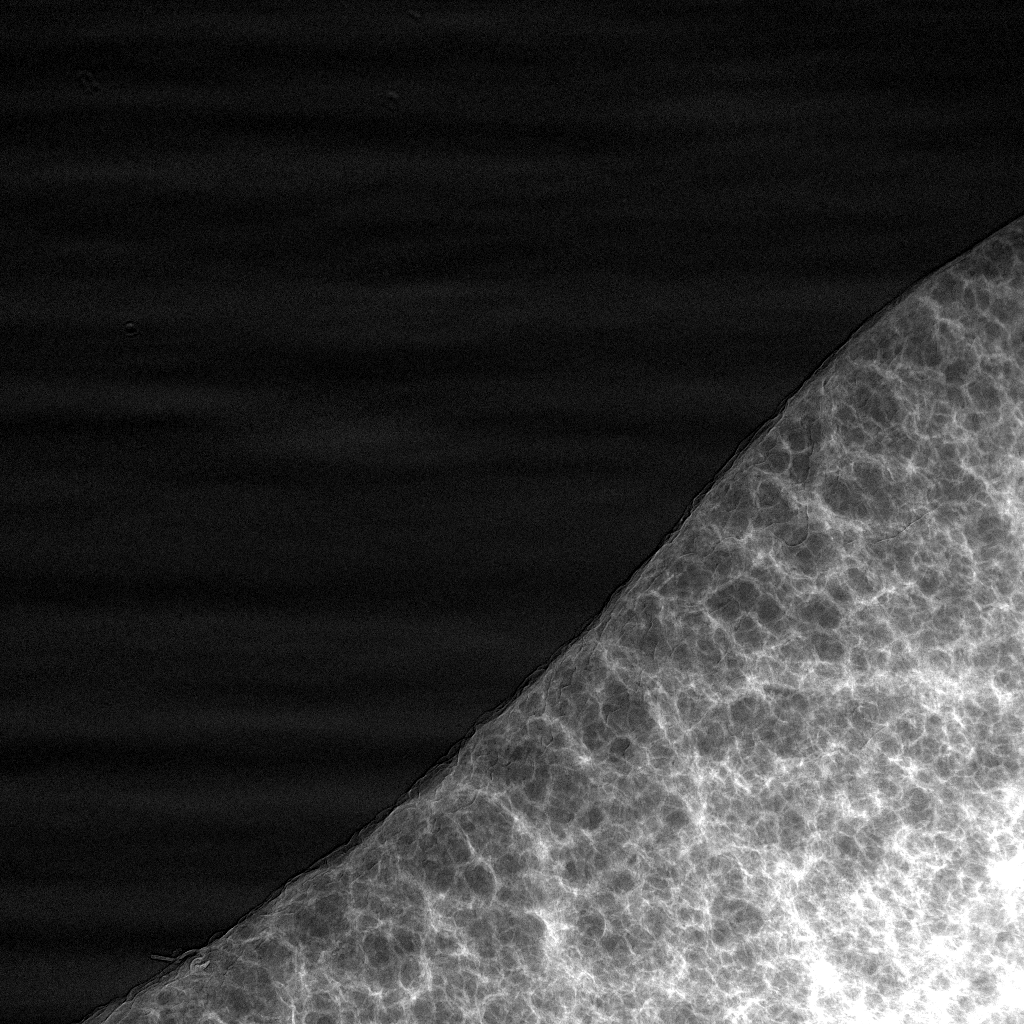
\includegraphics[width=\imagewidth]{img/merge/CP-R108C21Cb_s13358_normalize}};%
%					{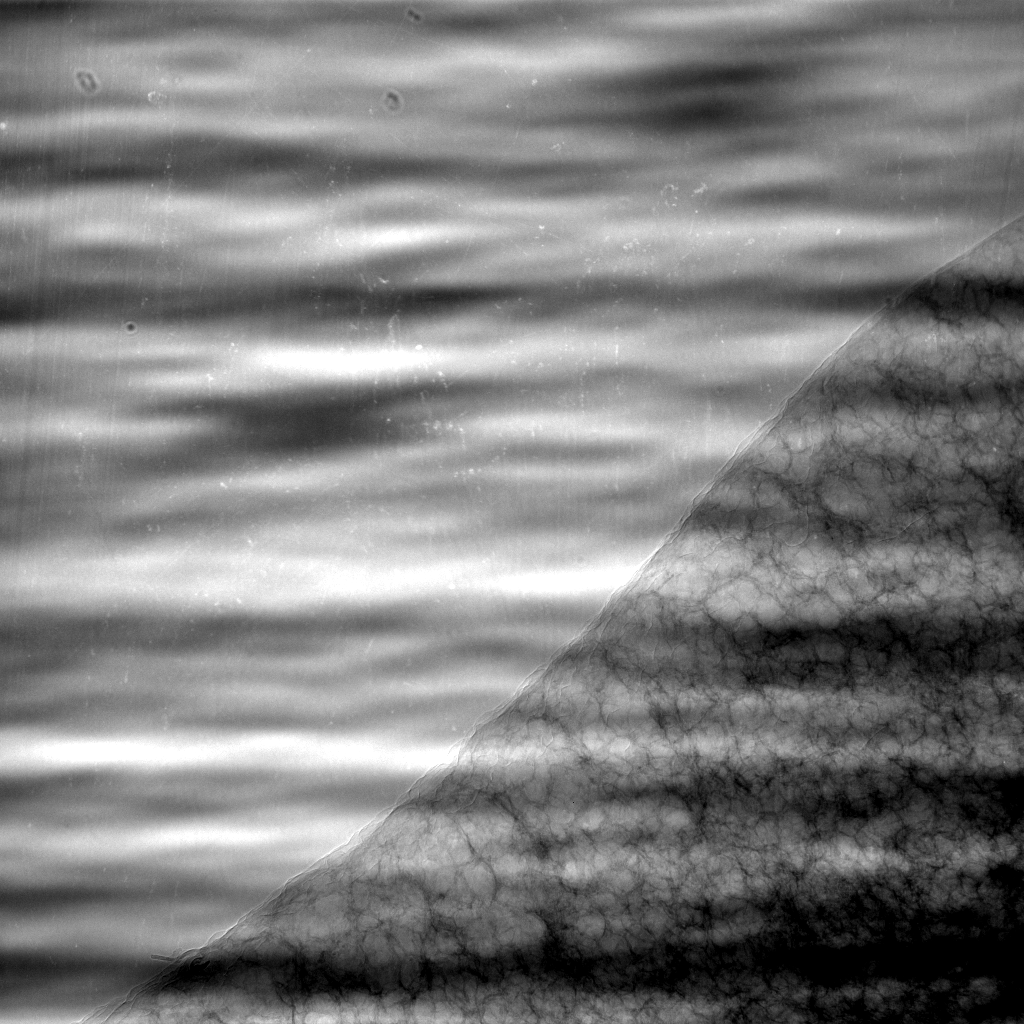
\includegraphics[width=\imagewidth]{R108C21Cb_s13358_normalize}};%
				\def\overlap{141}%
				\fill [red, nearly transparent] (1024-\overlap,1) rectangle (\size,\size);%
				\draw (1024-\overlap,1) rectangle (\size,\size);%
				\node [anchor=south west, color=white] at (0,1024) {(a)};				
			\end{tikzpicture}%
			\begin{tikzpicture}[x=\imagescale,y=-\imagescale]%
				\node[anchor=north west, inner sep=0pt, outer sep=0pt] at (0,0)%
					{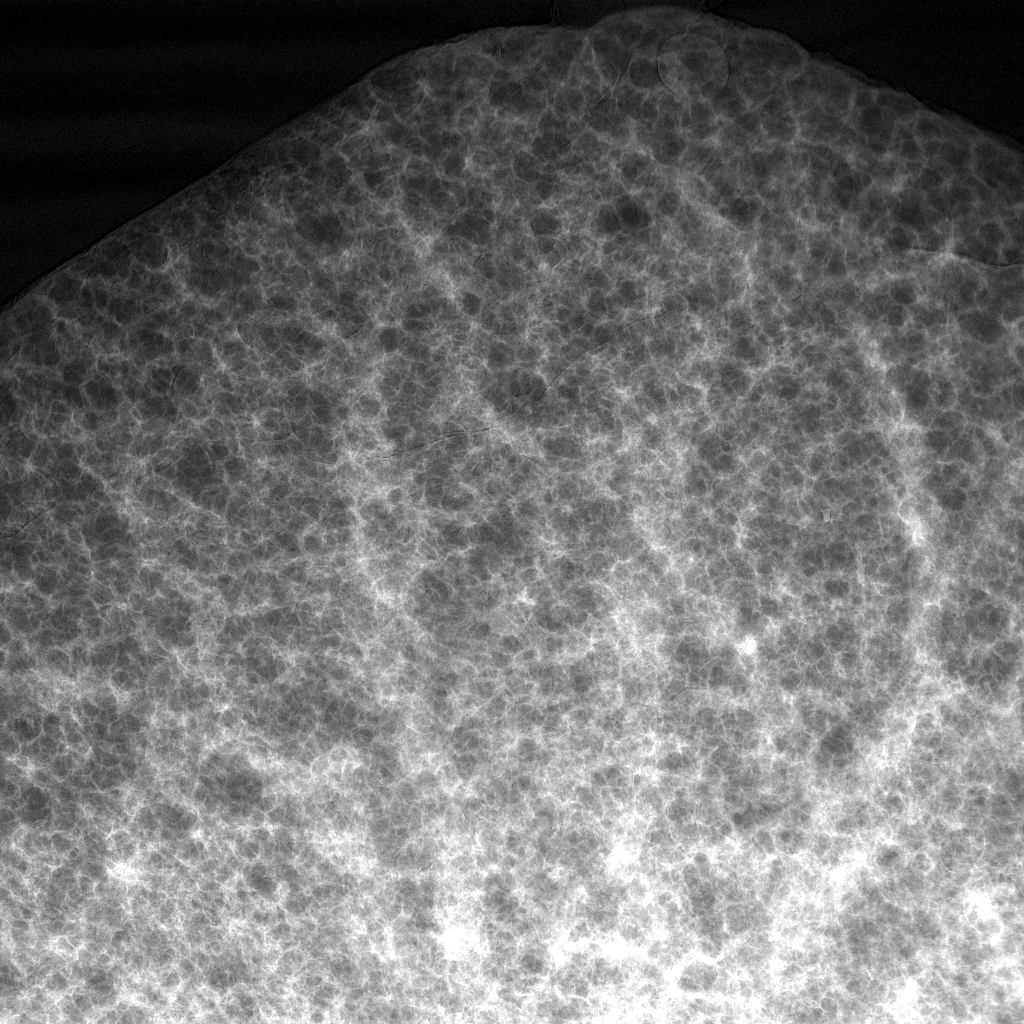
\includegraphics[width=\imagewidth]{img/merge/CP-R108C21Cb_s23358_normalize}};%
%					{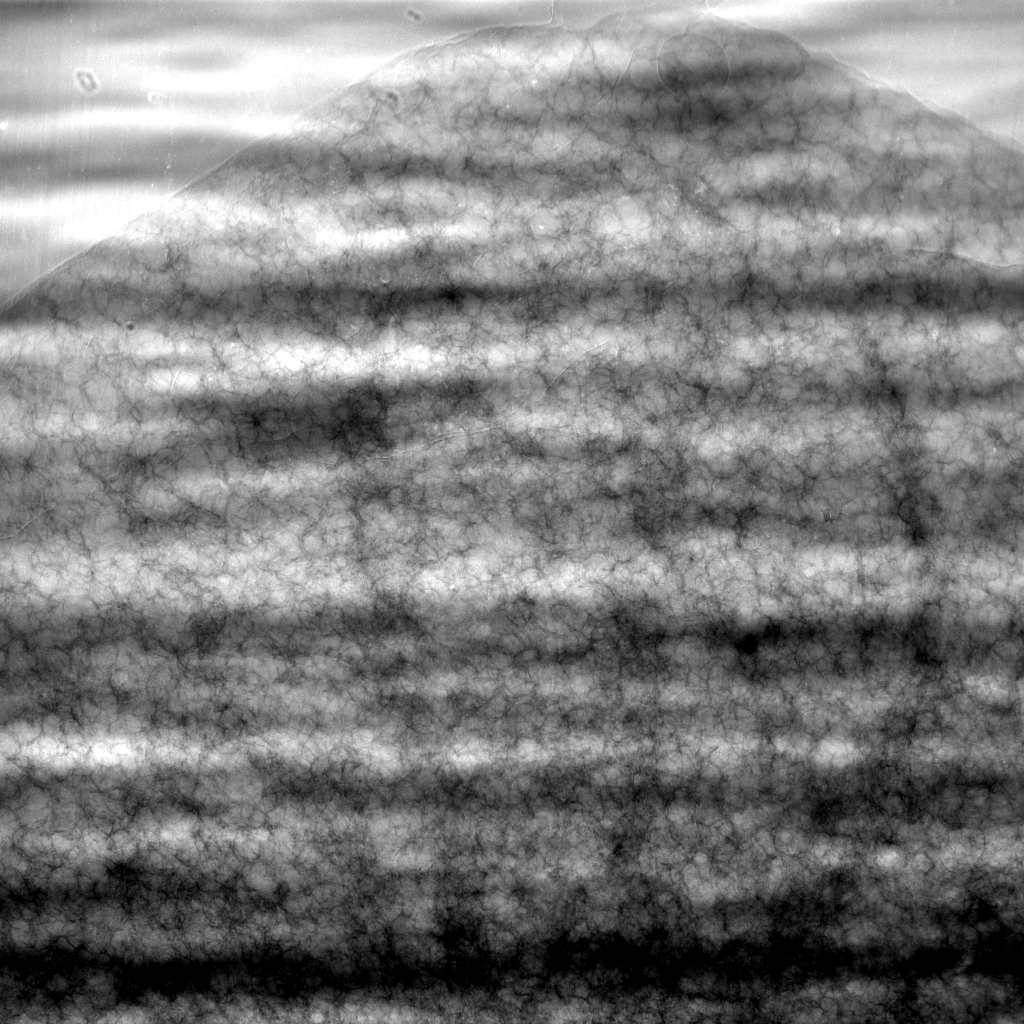
\includegraphics[width=\imagewidth]{R108C21Cb_s23358_normalize}};%
				\def\overlap{141}%
				\fill [green, nearly transparent] (1,1) rectangle (\overlap,\size);%
				\draw (1,1) rectangle (\overlap,\size);%
				\def\overlap{138}%
				\fill [blue, nearly transparent] (1024-\overlap,1) rectangle (\size,\size);%
				\draw (1024-\overlap,1) rectangle (\size,\size);%
			\end{tikzpicture}%
			\begin{tikzpicture}[x=\imagescale,y=-\imagescale]%
				% place image (integer coordinates refer to pixel centers):
				\node[anchor=north west, inner sep=0pt, outer sep=0pt] at (0,0)%
					{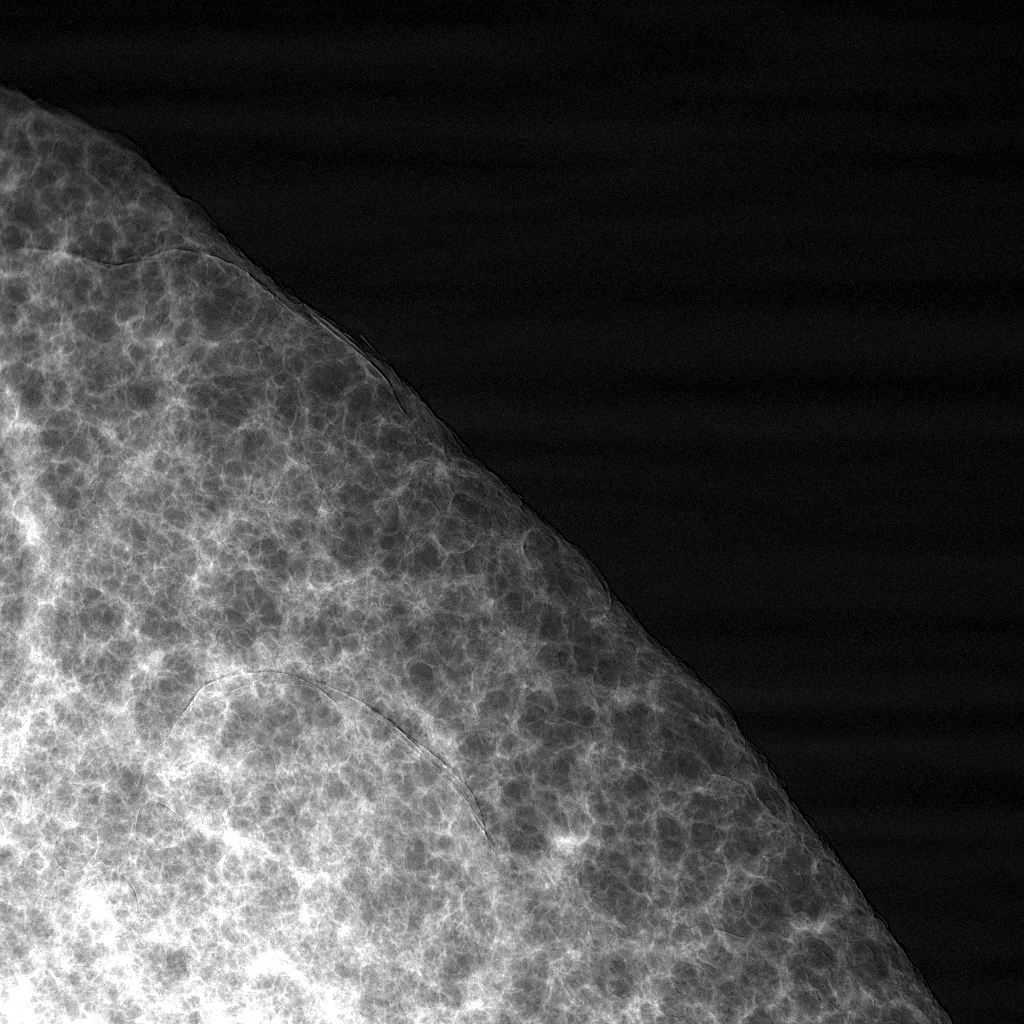
\includegraphics[width=\imagewidth]{img/merge/CP-R108C21Cb_s33358_normalize}};%
%					{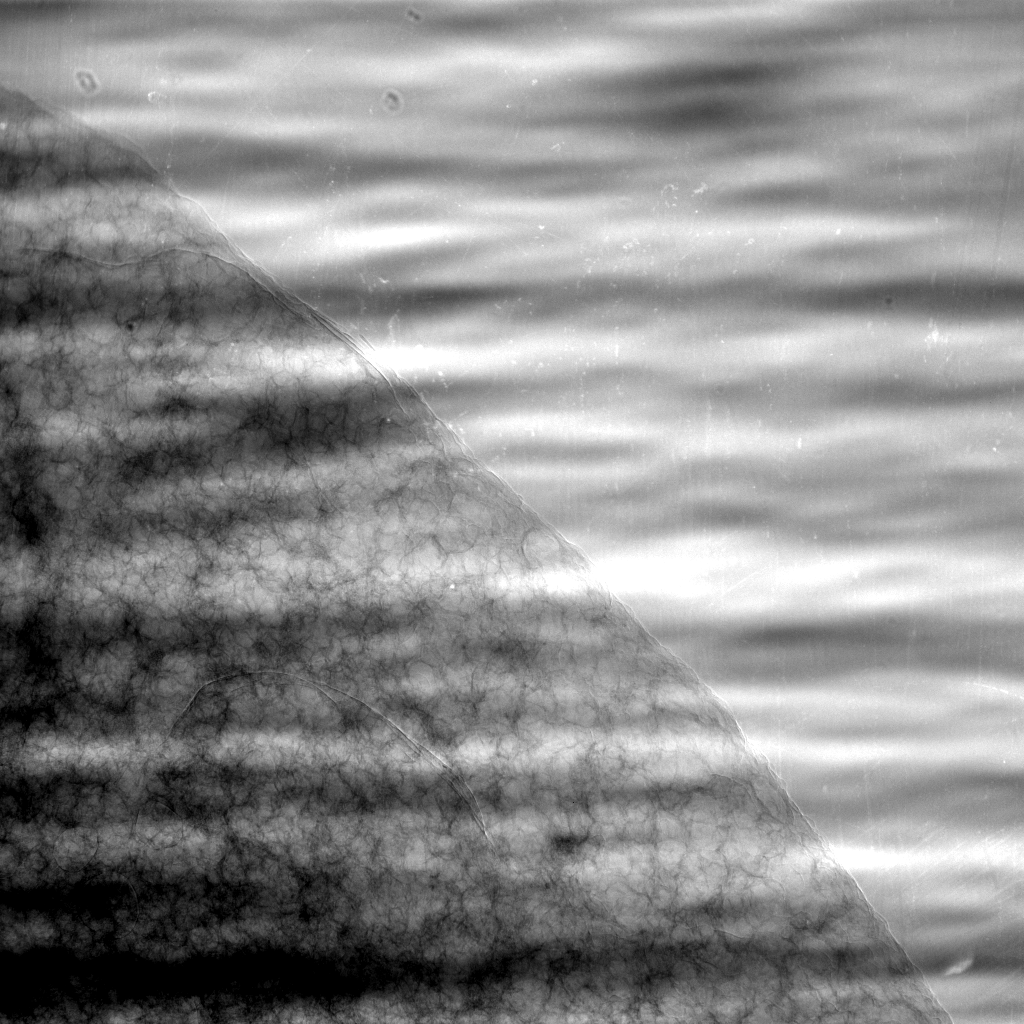
\includegraphics[width=\imagewidth]{R108C21Cb_s33358_normalize}};%
				\def\overlap{138}%
				\fill [yellow, nearly transparent] (1,1) rectangle (\overlap,\size);%
				\draw (1,1) rectangle (\overlap,\size);%
%				\draw[|-|,thick] (5,200) -- (1021,200) node [color=white,midway,above] {\SI{1.51552}{\milli\meter}};%
				\def\x{924}% 1024 - 100
				\def\y{922}% 1024 * .9 = 921.6
				\def\bar{338}% 100 px = 148 um
				\draw[|-|,thick, color=white] (\x-\bar,\y) -- (\x,\y) node [midway, above] {\SI{500}{\micro\meter}};%
			\end{tikzpicture}%
			\label{fig:subscans}%
%%%%%%%%%%%%%%%%%%%%%%%%%%%%%	
%	\caption{caption}
%\end{figure}
%\end{document}\\%
		%\documentclass{article}
%\usepackage{subfig}
%\usepackage{tikz}
%\usepackage{siunitx}
%\begin{document}
%\newcommand{\imsize}{\linewidth}
%\newlength\imagewidth % needed for scalebars
%\newlength\imagescale % needed for scalebars
%\begin{figure}
%	\centering
%%%%%%%%%%%%%%%%%%%%%%%%%%%%%
		\renewcommand{\imsize}{\linewidth}%
		\pgfmathsetlength{\imagewidth}{\imsize} % desired displayed width of image
		\pgfmathsetlength{\imagescale}{\imagewidth/2793}% pixel width of image
			\begin{tikzpicture}[x=\imagescale,y=-\imagescale]%
				\node[anchor=north west,inner sep=0pt,outer sep=0pt] at (0,0)%
					{\includegraphics[width=\imagewidth]{img/merge/R108C21Cb_mrg3333_normalize}};%
%					{\includegraphics[width=\imagewidth]{R108C21Cb_mrg3333_normalize}};%
				\def\x{2693} % 2793-100
				\def\y{922} % 1024*.9 = 921.6
				\def\bar{338} % 100 px = 148 um
				\draw[|-|,thick,color=white] (5,256) -- (2787,256) node [midway,above] {\SI{4.13364}{\milli\meter}};
				\draw[|-|,thick,color=white] (\x-\bar,\y) -- (\x,\y) node [midway,above] {\SI{500}{\micro\meter}};
				\node [anchor=center,color=white] at (100,1024-100) {b)};
				\end{tikzpicture}%
			\label{fig:merge-proj}%
%%%%%%%%%%%%%%%%%%%%%%%%%%%%%	
%	\caption{caption}
%\end{figure}
%\end{document}\\%
		%\documentclass{article}
%\usepackage{subfig}
%\usepackage{tikz}
%\usepackage{siunitx}
%\begin{document}
%\newcommand{\imsize}{\linewidth}
%\newlength\imagewidth % needed for scalebars
%\newlength\imagescale % needed for scalebars
%\begin{figure}
%	\centering
%%%%%%%%%%%%%%%%%%%%%%%%%%%%%
		\pgfmathsetlength{\imagewidth}{\imsize}%
		\pgfmathsetlength{\imagescale}{\imagewidth/2792}%
			\begin{tikzpicture}[x=\imagescale,y=-\imagescale]%
				\node [anchor=north west,inner sep=0pt,outer sep=0pt] at (0,0)%
					{\includegraphics[width=\imagewidth]{img/merge/R108C21Cb_mrg1024rec8bit}};% ``mogrify -shave 0x900 -format png R108C21Cb_mrg1024rec8bit.tif''
%					{\includegraphics[width=\imagewidth]{R108C21Cb_mrg1024rec8bit}};
				\clip (0,0) rectangle (2792,992);				
				\def\x{2692} % 2792-100
				\def\y{893} % 992 * .9 = 892.8
				\def\bar{338} % 100 px = 148 um
				%%%% scalebar
					\draw[|-|,thick,color=white] (\x-\bar,\y) -- (\x,\y) node [midway, above] {\SI{500}{\micro\meter}};
%					\draw[|-|,thick,color=white] (5,30) -- (2787,30) node [midway, below] {\SI{4.13216}{\milli\meter}};
				%%%% center
					\fill [color=red] (2792/2,992/2) circle (5);
				%%%% big circle
					\draw [dashed, ultra thick, color=red] (2792/2,992/2) circle (512);
					\def\angle{35}
					\draw [white, thick, <->] (2792/2,992/2) +(\angle:0) --  node (bigto) {} +(\angle:512); 
					\node [white] (bigfrom) at (349,256){$\frac{1024}{2}$px};
					\draw [white, ->, thick, densely dotted] (bigfrom) to [bend left=45] (bigto);
				%%%% big circle
				%%%% 141px circle
				\draw [dashed, ultra thick, color=red] (2792/2,992/2) circle (512-141);
				\def\angle{35+90}
					\draw [white,thick,<->] (2792/2,992/2) +(\angle:0) -- node (smallto) {} +(\angle:512-141);
					\node [white] (smallfrom) at (349,384) {$\frac{1024}{2}-141$px};
					\draw [white, ->, thick, densely dotted] (smallfrom) to [bend left=45] (smallto);
				%%%% 141px circle					
%				%%%% 138px circle
%				\draw [dashed,color=red] (2792/2,992/2) circle (512-138);
%				\def\angle{45+90+90}
%					\draw [white,<->] (2792/2,992/2) +(\angle:0) -- node (vsmallto) {} +(\angle:512-138);
%					\node [white] (vsmallfrom) at (2972-768,992-512) {$\frac{1024}{2}-138$px};
%					\draw [white,->,densely dotted] (vsmallfrom) to [bend right=45] (vsmallto);
%				%%%% 138px circle
				%%%% inset
%				\newcommand{\size}{.2\imagewidth}%
%				\clip (256,256) rectangle (512,512);
%				\node[anchor=north west,inner sep=0pt,outer sep=0pt] at (0,0)
%					{\includegraphics[width=\size]{R108C21Cb_mrg1024rec8bit}};
%					\draw[white] (0,0) rectangle (\size,-\size);
				%%%% inset
				\node [anchor=south west, color=white] at (0,990) {(c)};			
				\end{tikzpicture}%
			\label{fig:merge-rec}%
%%%%%%%%%%%%%%%%%%%%%%%%%%%%%	
%	\caption{caption}
%\end{figure}
%\end{document}\\%
	\end{figure}%
\else
	\begin{figure}[htp]%
		%\documentclass{article}
%\usepackage{subfig}
%\usepackage{tikz}
%\usepackage{siunitx}
%\begin{document}
%\newcommand{\imsize}{\linewidth}
%\newlength\imagewidth % needed for scalebars
%\newlength\imagescale % needed for scalebars
%\begin{figure}
%	\centering
%%%%%%%%%%%%%%%%%%%%%%%%%%%%%
	\renewcommand{\imsize}{.333\linewidth}
	\pgfmathsetlength{\imagewidth}{\imsize} % desired display width of image
	\pgfmathsetlength{\imagescale}{\imagewidth/1024} % pixel width of image
			% --------------------------------------------------------------
			% Cutline between SubScan 1 and 2: 141 pixels
			% Cutline between SubScan 2 and 3: 138 pixels
			% --------------------------------------------------------------
			\def\size{1023}%
			\begin{tikzpicture}[x=\imagescale,y=-\imagescale]%
				\node[anchor=north west, inner sep=0pt, outer sep=0pt] at (0,0)%
					{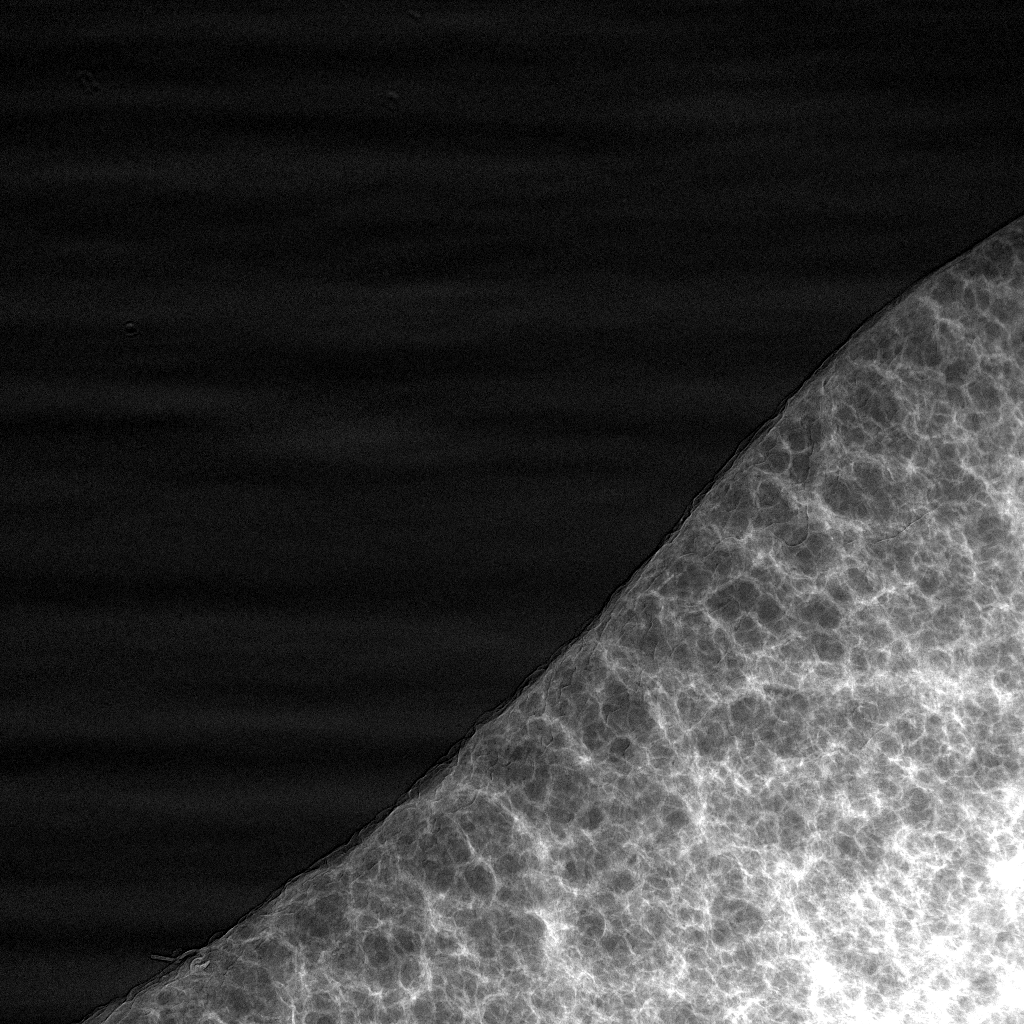
\includegraphics[width=\imagewidth]{img/merge/CP-R108C21Cb_s13358_normalize}};%
%					{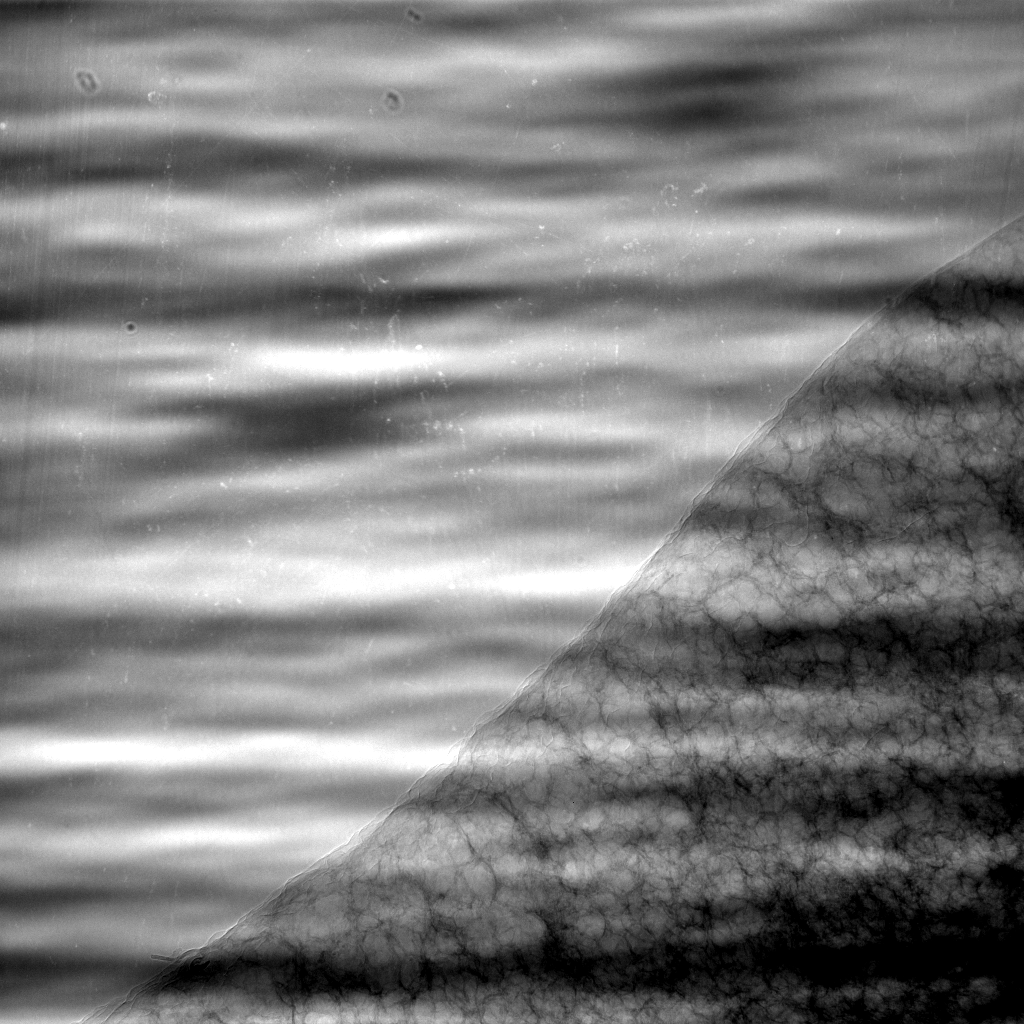
\includegraphics[width=\imagewidth]{R108C21Cb_s13358_normalize}};%
				\def\overlap{141}%
				\fill [red, nearly transparent] (1024-\overlap,1) rectangle (\size,\size);%
				\draw (1024-\overlap,1) rectangle (\size,\size);%
				\node [anchor=south west, color=white] at (0,1024) {(a)};				
			\end{tikzpicture}%
			\begin{tikzpicture}[x=\imagescale,y=-\imagescale]%
				\node[anchor=north west, inner sep=0pt, outer sep=0pt] at (0,0)%
					{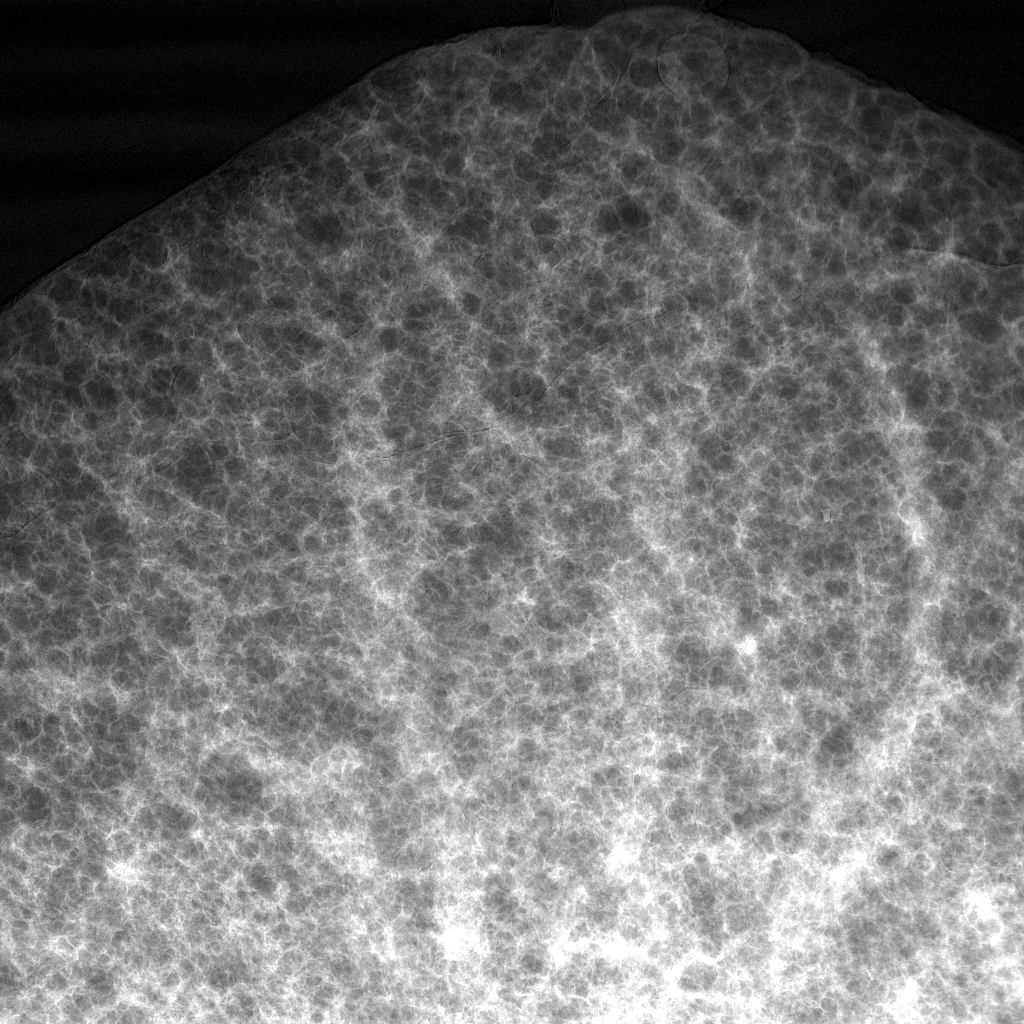
\includegraphics[width=\imagewidth]{img/merge/CP-R108C21Cb_s23358_normalize}};%
%					{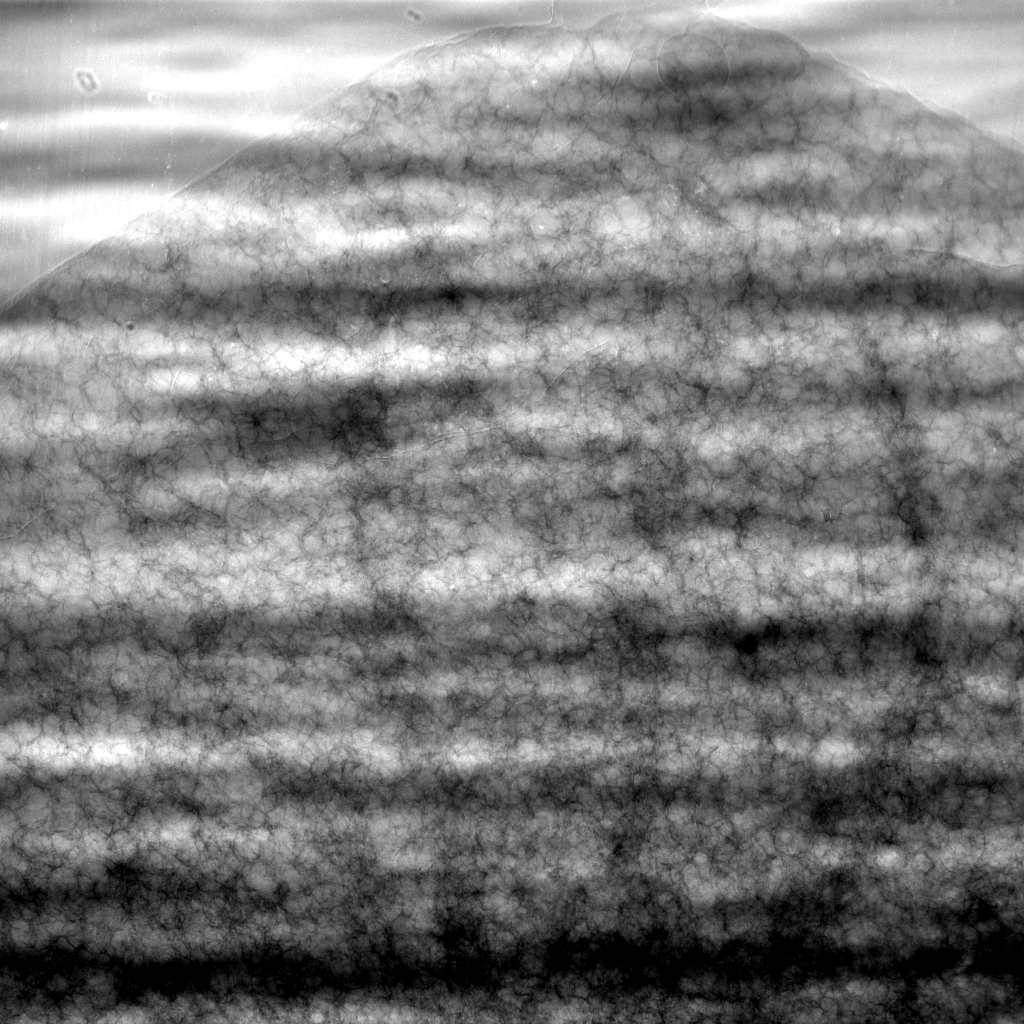
\includegraphics[width=\imagewidth]{R108C21Cb_s23358_normalize}};%
				\def\overlap{141}%
				\fill [green, nearly transparent] (1,1) rectangle (\overlap,\size);%
				\draw (1,1) rectangle (\overlap,\size);%
				\def\overlap{138}%
				\fill [blue, nearly transparent] (1024-\overlap,1) rectangle (\size,\size);%
				\draw (1024-\overlap,1) rectangle (\size,\size);%
			\end{tikzpicture}%
			\begin{tikzpicture}[x=\imagescale,y=-\imagescale]%
				% place image (integer coordinates refer to pixel centers):
				\node[anchor=north west, inner sep=0pt, outer sep=0pt] at (0,0)%
					{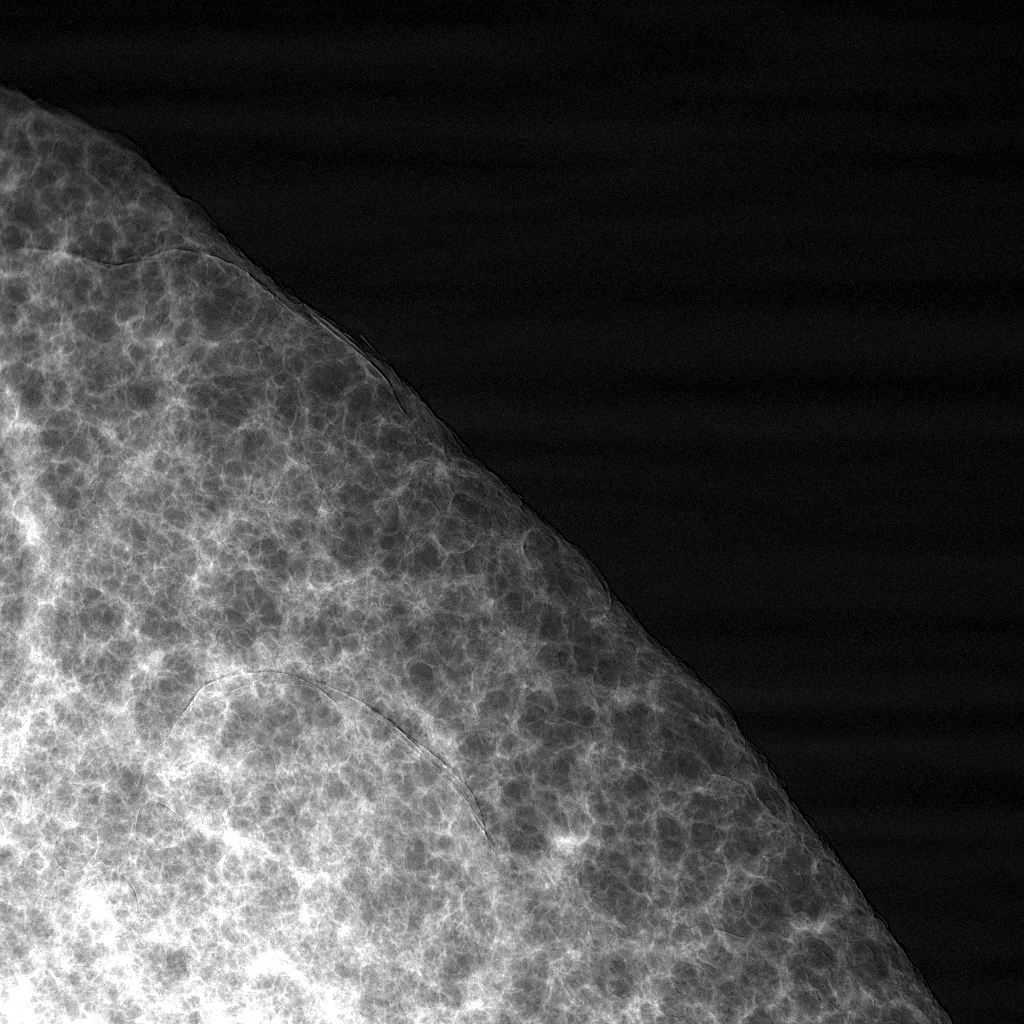
\includegraphics[width=\imagewidth]{img/merge/CP-R108C21Cb_s33358_normalize}};%
%					{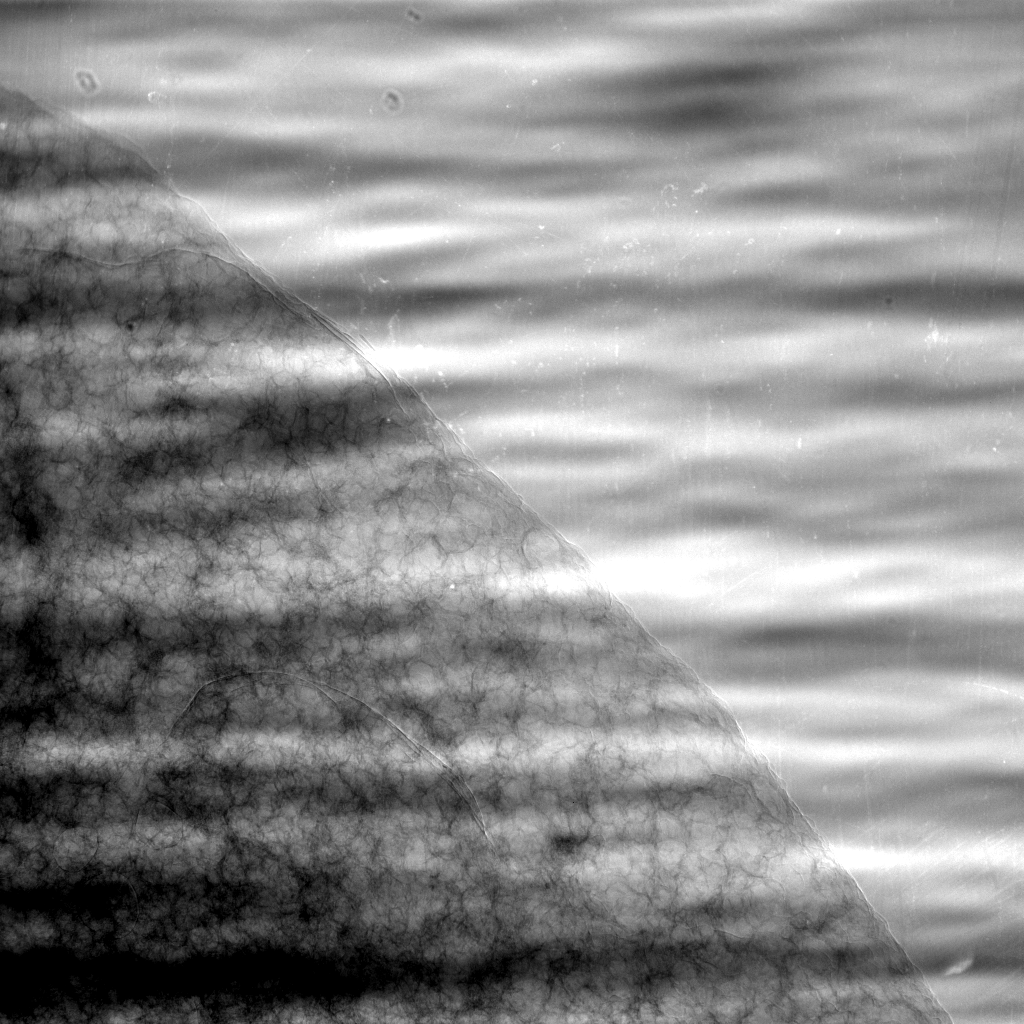
\includegraphics[width=\imagewidth]{R108C21Cb_s33358_normalize}};%
				\def\overlap{138}%
				\fill [yellow, nearly transparent] (1,1) rectangle (\overlap,\size);%
				\draw (1,1) rectangle (\overlap,\size);%
%				\draw[|-|,thick] (5,200) -- (1021,200) node [color=white,midway,above] {\SI{1.51552}{\milli\meter}};%
				\def\x{924}% 1024 - 100
				\def\y{922}% 1024 * .9 = 921.6
				\def\bar{338}% 100 px = 148 um
				\draw[|-|,thick, color=white] (\x-\bar,\y) -- (\x,\y) node [midway, above] {\SI{500}{\micro\meter}};%
			\end{tikzpicture}%
			\label{fig:subscans}%
%%%%%%%%%%%%%%%%%%%%%%%%%%%%%	
%	\caption{caption}
%\end{figure}
%\end{document}\\%
		%\documentclass{article}
%\usepackage{subfig}
%\usepackage{tikz}
%\usepackage{siunitx}
%\begin{document}
%\newcommand{\imsize}{\linewidth}
%\newlength\imagewidth % needed for scalebars
%\newlength\imagescale % needed for scalebars
%\begin{figure}
%	\centering
%%%%%%%%%%%%%%%%%%%%%%%%%%%%%
		\renewcommand{\imsize}{\linewidth}%
		\pgfmathsetlength{\imagewidth}{\imsize} % desired displayed width of image
		\pgfmathsetlength{\imagescale}{\imagewidth/2793}% pixel width of image
			\begin{tikzpicture}[x=\imagescale,y=-\imagescale]%
				\node[anchor=north west,inner sep=0pt,outer sep=0pt] at (0,0)%
					{\includegraphics[width=\imagewidth]{img/merge/R108C21Cb_mrg3333_normalize}};%
%					{\includegraphics[width=\imagewidth]{R108C21Cb_mrg3333_normalize}};%
				\def\x{2693} % 2793-100
				\def\y{922} % 1024*.9 = 921.6
				\def\bar{338} % 100 px = 148 um
				\draw[|-|,thick,color=white] (5,256) -- (2787,256) node [midway,above] {\SI{4.13364}{\milli\meter}};
				\draw[|-|,thick,color=white] (\x-\bar,\y) -- (\x,\y) node [midway,above] {\SI{500}{\micro\meter}};
				\node [anchor=center,color=white] at (100,1024-100) {b)};
				\end{tikzpicture}%
			\label{fig:merge-proj}%
%%%%%%%%%%%%%%%%%%%%%%%%%%%%%	
%	\caption{caption}
%\end{figure}
%\end{document}\\%
		%\documentclass{article}
%\usepackage{subfig}
%\usepackage{tikz}
%\usepackage{siunitx}
%\begin{document}
%\newcommand{\imsize}{\linewidth}
%\newlength\imagewidth % needed for scalebars
%\newlength\imagescale % needed for scalebars
%\begin{figure}
%	\centering
%%%%%%%%%%%%%%%%%%%%%%%%%%%%%
		\pgfmathsetlength{\imagewidth}{\imsize}%
		\pgfmathsetlength{\imagescale}{\imagewidth/2792}%
			\begin{tikzpicture}[x=\imagescale,y=-\imagescale]%
				\node [anchor=north west,inner sep=0pt,outer sep=0pt] at (0,0)%
					{\includegraphics[width=\imagewidth]{img/merge/R108C21Cb_mrg1024rec8bit}};% ``mogrify -shave 0x900 -format png R108C21Cb_mrg1024rec8bit.tif''
%					{\includegraphics[width=\imagewidth]{R108C21Cb_mrg1024rec8bit}};
				\clip (0,0) rectangle (2792,992);				
				\def\x{2692} % 2792-100
				\def\y{893} % 992 * .9 = 892.8
				\def\bar{338} % 100 px = 148 um
				%%%% scalebar
					\draw[|-|,thick,color=white] (\x-\bar,\y) -- (\x,\y) node [midway, above] {\SI{500}{\micro\meter}};
%					\draw[|-|,thick,color=white] (5,30) -- (2787,30) node [midway, below] {\SI{4.13216}{\milli\meter}};
				%%%% center
					\fill [color=red] (2792/2,992/2) circle (5);
				%%%% big circle
					\draw [dashed, ultra thick, color=red] (2792/2,992/2) circle (512);
					\def\angle{35}
					\draw [white, thick, <->] (2792/2,992/2) +(\angle:0) --  node (bigto) {} +(\angle:512); 
					\node [white] (bigfrom) at (349,256){$\frac{1024}{2}$px};
					\draw [white, ->, thick, densely dotted] (bigfrom) to [bend left=45] (bigto);
				%%%% big circle
				%%%% 141px circle
				\draw [dashed, ultra thick, color=red] (2792/2,992/2) circle (512-141);
				\def\angle{35+90}
					\draw [white,thick,<->] (2792/2,992/2) +(\angle:0) -- node (smallto) {} +(\angle:512-141);
					\node [white] (smallfrom) at (349,384) {$\frac{1024}{2}-141$px};
					\draw [white, ->, thick, densely dotted] (smallfrom) to [bend left=45] (smallto);
				%%%% 141px circle					
%				%%%% 138px circle
%				\draw [dashed,color=red] (2792/2,992/2) circle (512-138);
%				\def\angle{45+90+90}
%					\draw [white,<->] (2792/2,992/2) +(\angle:0) -- node (vsmallto) {} +(\angle:512-138);
%					\node [white] (vsmallfrom) at (2972-768,992-512) {$\frac{1024}{2}-138$px};
%					\draw [white,->,densely dotted] (vsmallfrom) to [bend right=45] (vsmallto);
%				%%%% 138px circle
				%%%% inset
%				\newcommand{\size}{.2\imagewidth}%
%				\clip (256,256) rectangle (512,512);
%				\node[anchor=north west,inner sep=0pt,outer sep=0pt] at (0,0)
%					{\includegraphics[width=\size]{R108C21Cb_mrg1024rec8bit}};
%					\draw[white] (0,0) rectangle (\size,-\size);
				%%%% inset
				\node [anchor=south west, color=white] at (0,990) {(c)};			
				\end{tikzpicture}%
			\label{fig:merge-rec}%
%%%%%%%%%%%%%%%%%%%%%%%%%%%%%	
%	\caption{caption}
%\end{figure}
%\end{document}%
		\caption{%
			Wide field scan of a rat lung sample obtained from a Sprague-Dawley rat 21 days after birth, showing the distal-medial edge of the right lower lung lobe. The sample was scanned at \SI{12.6}{\kilo\electronvolt}, according to protocol B, as described in table~\ref{tab:protocols}. %
			(a) Three corrected and independently acquired projection images from subscans $s_1$--$s_3$, each with a size of 1024\(\times\)1024 pixels at a resolution of \SI{1.48}{\micro\meter} per pixel, each covering a field of view of \SI{1.52}{\milli\meter}. Subscans $s_1$ and $s_2$ overlap each other by 141 pixels (red and green overlay), subscans $s_2$ and $s_3$ overlap each other by 138 pixels (blue and yellow overlay). 5244 projections over a rotation of \SI{180}{\degree} have been acquired for all subscans. %
			(b) Merged projection obtained from the three subscans shown in subfigure (a). Each merged projection has a size of 2793\(\times\)1024 pixels at a pixel size of \SI{1.48}{\micro\meter}. The width of the merged projections is slightly smaller than three times the width of the subscans, due to the overlap required to merge the projections (2793px=3072px-141px-138px). %
			(c) Cropped slice of the tomographic dataset, reconstructed from 5244 merged projections shown in subfigure b). The dashed red circles mark the start and end of the overlap region. Due to the coherence of the x-ray beam, the air-to-paraffin interface is visible around the sample.%
			}%
		\label{fig:wide field scan results}%
	\end{figure}
\fi

\subsection{Increasing the field of view}
The field of view of \SI{1.56}{\milli\meter}$\times$\SI{1.56}{\milli\meter} with a voxel size of \SI{0.74}{\micro\meter} at TOMCAT did permit visualizations of an entire acinus. Increasing the field of view by three times solved this limitation, allowing us to obtain three-dimensional reconstructions of full acini.

Figure~\ref{fig:s2-wfs} compares reconstructions of a conventional scan with reconstructions of a wide field scan. For a conventional scan (shown in fig.~\ref{fig:s2-wfs}(a)), the multiple acini in the sample are only partially contained inside the dataset (green and red airway segment). Increasing the field of view (fig.~\ref{fig:s2-wfs}(b)) allows the visualization of the full extent of those acini. Additionally, a third acinus (yellow) which is not visible inside the field of view of a conventional scan, can be visualized.

\ifiucr
	%\onecolumn
	\begin{figure}%
		\centering%
		\caption{three-dimensional visualization of the distal-medial tip of the right lower lung lobe of a Sprague Dawley rat. The gray structure in the background shows a semitransparent view of the sample with segmented airways. The foreground shows isosurfaces of terminal airways that have been extracted using a threshold interval based region growing algorithm. (a): Conventional scan; the extracted airway segments (green and red) are only partially contained inside the total sample volume. (b): Wide field scan with increased field of view; the green and red segment show multiple full acini inside the dataset, the yellow segment contains a partial acinus. The segmentation is only limited by the sample size and not by the field of view of the tomographic scan.}%
		\label{fig:s2-wfs}%
		\renewcommand{\imsize}{\linewidth}%
		\pgfmathsetlength{\imagewidth}{\imsize}%
		\pgfmathsetlength{\imagescale}{\imagewidth/1202}%
		\def\x{250}% scalebar-x at golden ratio of x=1202px (=743)
		\def\y{575}% scalebar-y at 90% of height of y=680px (=612)
		\begin{tikzpicture}[x=\imagescale,y=-\imagescale]
			\node[anchor=north west, inner sep=0pt, outer sep=0pt] at (0,0)
				{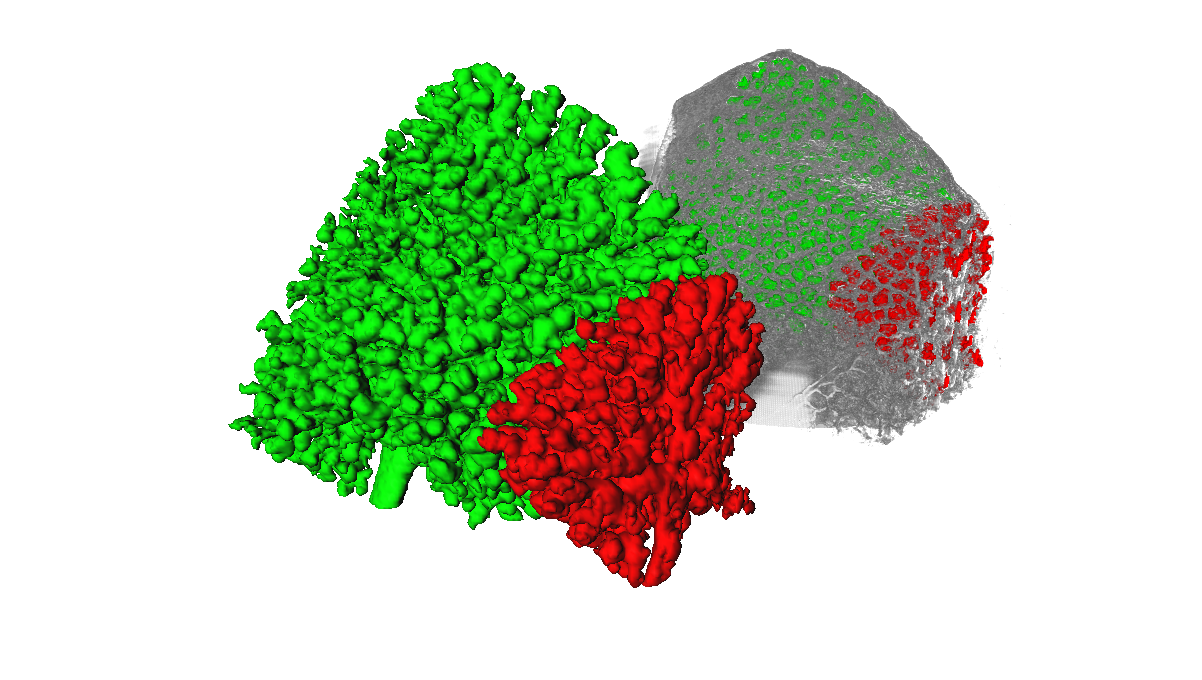
\includegraphics[width=\imagewidth]{img/widefieldscanning/R108C04C-overview-s2}};
			% 423px = 1.5155mm > 100px = 358um > 140px = 500um
			% \draw[|-|,thick] (238,388) -- (638,527) node [white,sloped,midway,above] {\SI{1.5155}{\milli\meter} (1024px)};
			\draw[|-|,thick] (\x,\y) -- (\x+140,\y) node [midway, above] {\SI{500}{\micro\meter}};
			\node [anchor=south west] at (0,680) {(a)};
		\end{tikzpicture}%
		\\%
		\begin{tikzpicture}[x=\imagescale,y=-\imagescale]
			\node[anchor=north west, inner sep=0pt, outer sep=0pt] at (0,0)
				{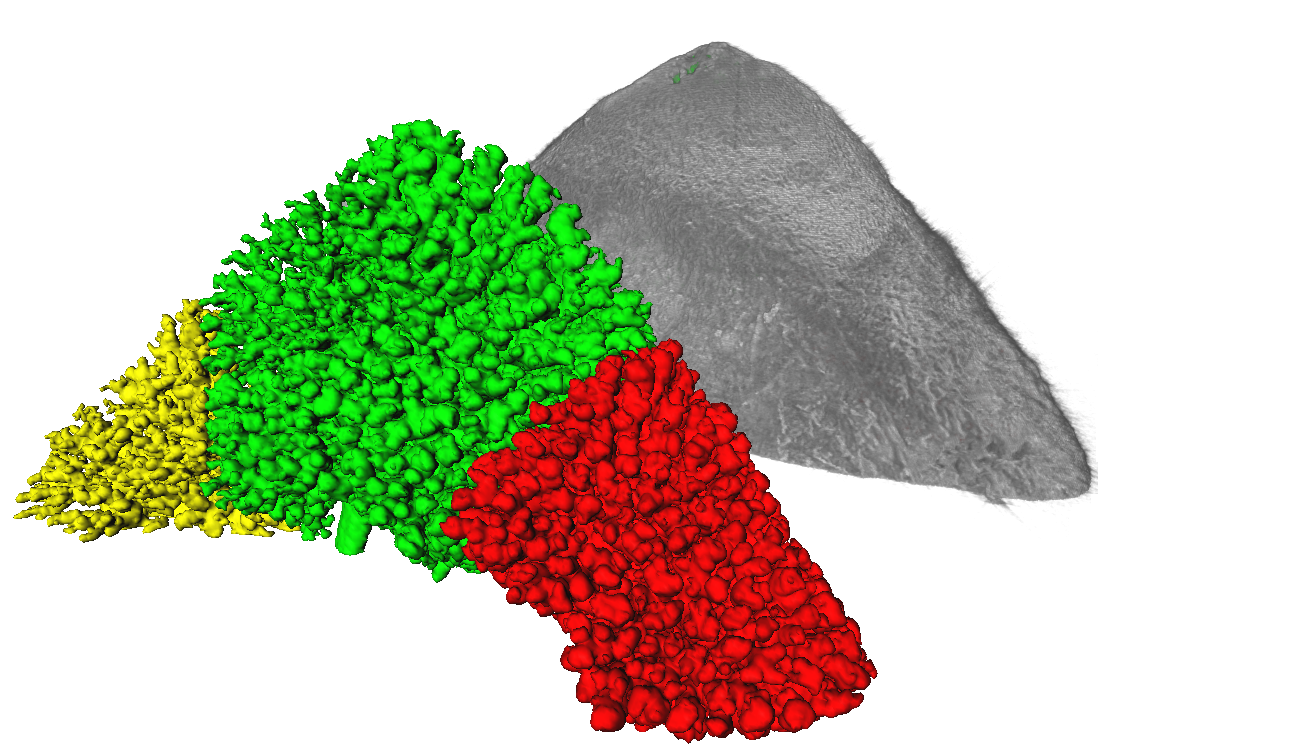
\includegraphics[width=\imagewidth]{img/widefieldscanning/R108C04C-overview-merge}};
			% 423px = 1.5155mm > 100px = 358um > 140px = 500um
			%\draw[|-|,thick] (238,388) -- (638,527) node [white,sloped,midway,above] {\SI{1.5155}{\milli\meter} (1024px)};
			\draw[|-|,thick] (\x,\y) -- (\x+280,\y) node [midway, above] {\SI{1}{\milli\meter}};
			\node [anchor=south west] at (0,680) {(b)};
		\end{tikzpicture}%
	\end{figure}%
	%\twocolumn
\else
	\begin{figure}[htp]%
	\renewcommand{\imsize}{\linewidth}%
	\pgfmathsetlength{\imagewidth}{\imsize}% desired displayed width of image
	\pgfmathsetlength{\imagescale}{\imagewidth/1202}% pixel width of imagefile used below
		\centering%
		\def\x{250}%
		\def\y{575}%
		\subfloat[Conventional scan]{%
			\label{subfig:overview-s2}%
			\begin{tikzpicture}[x=\imagescale,y=-\imagescale]
				\node[anchor=north west, inner sep=0pt, outer sep=0pt] at (0,0)
					{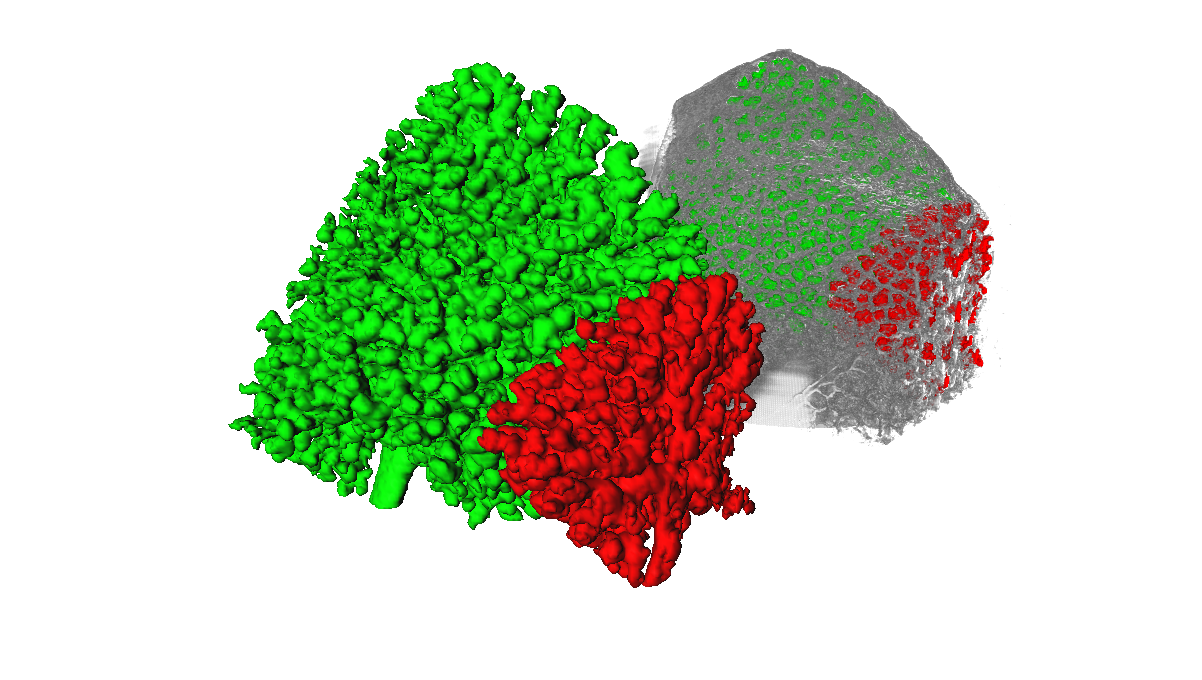
\includegraphics[width=\imagewidth]{img/widefieldscanning/R108C04C-overview-s2}};
				% 510px = 1.5155mm > 100px = 297um > 168px = 500um
				\draw[|-|,thick] (244,367) -- (718,554) node [sloped,midway,above] {\SI{1.5155}{\milli\meter}};
				\draw[|-|,thick] (\x,\y) -- (\x+168,\y) node [midway, above] {\SI{500}{\micro\meter}};
			\end{tikzpicture}%
		}\\%
		\def\x{150}%
		\def\y{575}%
		\subfloat[Scan with increased field of view]{%
			\label{subfig:overview-merge}%
			\begin{tikzpicture}[x=\imagescale,y=-\imagescale]
				\node[anchor=north west, inner sep=0pt, outer sep=0pt] at (0,0)
					{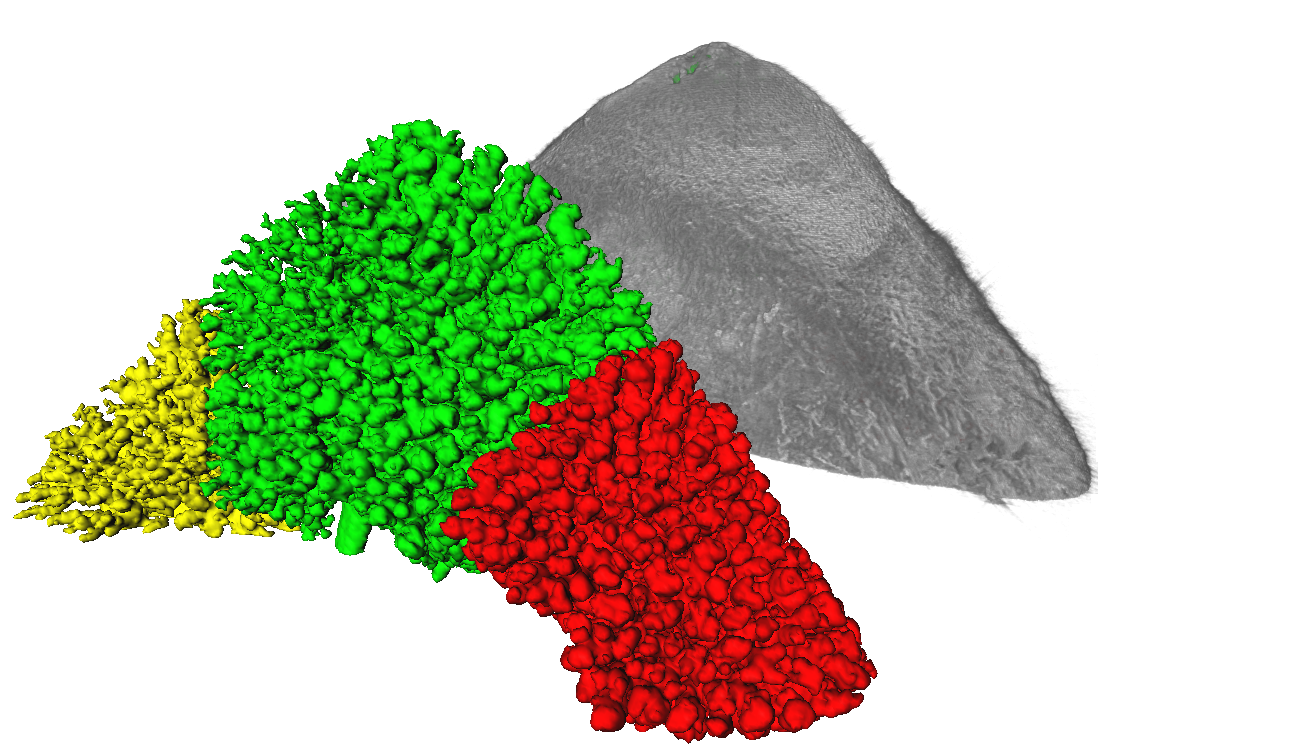
\includegraphics[width=\imagewidth]{img/widefieldscanning/R108C04C-overview-merge}};
				% 906px = 4.0641mm > 100px = 449um > 111px = 500um
				\draw[|-|,thick] (39,454) -- (923,653) node [sloped,midway,above] {\SI{4.0641}{\milli\meter}};
				\draw[|-|,thick] (\x,\y) -- (\x+222,\y) node [midway, above] {\SI{1}{\milli\meter}};
			\end{tikzpicture}%
		}%
		\caption{three-dimensional visualization of the distal-medial tip of the right lower lung lobe of a Sprague Dawley rat. The gray structure in the background shows a semitransparent view of the sample with segmented airways. The foreground shows isosurfaces of terminal airways that have been extracted using a threshold interval based region growing algorithm. (a): Conventional scan; the extracted airway segments (green and red) are only partially contained inside the total sample volume. (b): Wide field scan with increased field of view; the green and red segment show multiple full acini inside the dataset, the yellow segment contains a partial acinus. The segmentation is only limited by the sample size and not by the field of view of the tomographic scan.}%
		\label{fig:s2-wfs}%
	\end{figure}
\fi

\subsection{Quality guided protocols}
\label{subsec:quality-guided-protocols}
Nineteen different protocols were defined (details see table~\ref{tab:protocols}). These protocols were linearly scaled in total amount of projections from an oversampled gold standard scan down to \SI{16}{\percent} of acquired projections. Choosing one of these protocols enables the end-user to perform a scan with reduced total time while still being able to reconstruct his or her sample in three-dimensions (as discussed later).

Protocol A would correspond to a gold standard scan covering the chosen field of view, with nine independent local tomography scans with a field of view of 1024$\times$1024 pixels each. This protocol was omitted from this study, since the sampling theorem can be equally satisfied by acquiring the required amount of projections with one central and two ring scans, as defined in section~\ref{subsubsec:reduction-of-acquisition-time}. Including an overlap of 100 pixels between the central and the ring scan, 13534 projections need to be acquired for the gold-standard protocol ($P_{A}=3(3072-200)\frac{\pi}{2}$).

Protocols C--T have been linearly scaled down with a decreasing percentage of acquired projections of the ring scans. As mentioned before, to facilitate the stitching of the individual projections, the amount of projections obtained for the central scan is reduced by a factor of two compared to the amount of projections recorded for the ring scans. As a consequence of the scaling and division by two, Protocol B actually corresponds to an oversampling of \SI{16}{\percent} as compared to a gold standard scan.

\begin{table}
	\caption{Specification of different protocols: Protocol A corresponds to the Gold Standard, and would be required to cover the field of view with 9 independent scans with a detector width of 1024 pixels (plus an overlap of 100 pixels), resulting in a number of projections $P_{A}=9*(1024-100)\ifhtml \pi/2 \else \frac{\pi}{2} \fi= 13020$. The gold standard wide field scanning protocol would correspond to covering the desired field of view with nine independent scans, resulting in a total number of projections of $P_{A} = 3(3072-200)\ifhtml \pi/2 \else \frac{\pi}{2} \fi= 13534$. Three-dimensional reconstructions of the datasets marked with a light gray background are shown in figure~\ref{fig:BvsT}.}%
	\label{tab:protocols}%
	\begin{tabular}{cccccc}%
		\multirow{2}{*}{Protocol} & \multicolumn{3}{c}{Projections for Subscan} & Total Number		& Time/Radiation\\
		        				  & $s_{1}$ & $s_{2}$ & $s_{3}$ 				& of Projections	& Dose [\%]\\%
		\hline
		A\footnote{Gold Standard} & & &    & 13534 & 100\\%
		\rowcolor{lightgray} B & 5244 & 5244 & 5244 & 15732 & 116\\%
		C & 5244 & 2622 & 5244 & 13110 &  97\\%
		D & 4370 & 4370 & 4370 & 13110 &  97\\%
		E & 4370 & 2185 & 4370 & 10925 &  81\\%
		F & 3934 & 3934 & 3934 & 11802 &  87\\%
		G & 3934 & 1967 & 3934 & 9835  &  73\\%
		H & 3496 & 3496 & 3496 & 10488 &  77\\%
		I & 3496 & 1748 & 3496 & 8740  &  65\\%
		J & 3060 & 3060 & 3060 & 9180  &  68\\%
		K & 3060 & 1530 & 3060 & 7650  &  57\\%
		\rowcolor{lightgray} L & 2622 & 2622 & 2622 & 7866  &  58\\%
		M & 2622 & 1311 & 2622 & 6555  &  48\\%
		N & 2186 & 2186 & 2186 & 6558  &  48\\%
		O & 2185 & 1093 & 2185 & 5463  &  40\\%
		P & 1748 & 1748 & 1748 & 5244  &  39\\%
		Q & 1748 & 874  & 1748 & 4370  &  32\\%
		R & 1312 & 1312 & 1312 & 3936  &  29\\%
		S & 874  & 874  & 874  & 2622  &  19\\%
		\rowcolor{lightgray} T & 874  & 437  & 874  & 2185  &  16\\%
	\end{tabular}%
\end{table}

A reduction of the total acquisition time by \SI{84}{\percent} compared to the gold standard was achieved, as shown in table~\ref{tab:protocols}. The same rat lung sample was batch-scanned with each of the 19 protocols. Three-dimensional reconstructions and visualizations have been made to assess the artifacts that arise through the reduction of the number of projections.

The performance of the protocols was been quantified using the difference image of binarized slices of the tomographic datasets, segmented according to%
\ifhtml%
	~\citet{Otsu1979}%
\else%
	~\citeasnoun{Otsu1979}%
\fi%
. The difference value ($E_{norm}$) plotted in figure~\ref{fig:NormalizedErrorPlot} was calculated for each protocol $i=$1--19 according to equations~\ref{eq:errorcalculation-a}--\ref{eq:errorcalculation-c}. Using a thresholded slice $k$ of each protocol $i$ ($Slice_{i_{k}}$) and the corresponding slice $k$ of the gold standard protocol $B$ ($Slice_{B_{i}}$) the absolute difference image ($D_{i_{k}}$) of these two slices $k$ was calculated. The sum of all pixels of this difference image yields a value ($E_{i_{norm_{k}}}$) for the difference of the examined slice $k$ of protocol $i$ with the corresponding slice of the gold standard protocol B.
\begin{eqnarray}%
	D_{i_{k}} &=& |Slice_{B_{k}}-Slice_{i_{k}}|\label{eq:errorcalculation-a}\\%
	E_{i_{norm_{k}}} &=& \sum_{x}\sum_{y} D_{i_{k}}\label{eq:errorcalculation-b}\\%
	E_{i_{norm}} &=& \overline{E_{i_{norm_{k}}}}\label{eq:errorcalculation-c}%
\end{eqnarray}%

This combined difference value ($E_{i_{norm_{k}}}$) was calculated for 205 regularly spaced slices (%
%$i=1:5:1024$%
every fifth slice%
) of the full dataset. The mean ($\overline{E_{i_{norm_{k}}}}$) difference value for all slices was normalized to the scanned quality-steps from 16.14--\SI{116.24}{\percent} (as stated in table~\ref{tab:protocols}) and plotted as max$(E_{norm}-E_{i_{norm}})$ with its standard deviation ($\sigma(E_{i_{norm_{k}}})$). The normalization and inversion was carried out to make the experimentally derived values (blue diamonds) directly comparable to the values obtained from the computed set of protocols (as specified in section~\ref{subsec:wfs-setup}, red dots).

As can be seen in figure~\ref{fig:NormalizedErrorPlot}, the calculated quality of the reconstructions from the different protocols decreases as amount of total obtained projections decreases, as expected. The calculated error of the different protocols, compared to a gold standard protocol (blue diamonds) shows experimental results not derived using simulations with a phantom, but rather real data obtained from actual scans of lung tissue. The plots for the simulation and the normalized difference value are not perfectly in agreement, but show the same trend. The simulation shows an exponential decrease in quality, while the calculated, normalized error shows a more linear decrease in quality from protocol B towards protocol T.

\ifiucr
	\begin{figure}%
		\centering%
		\caption{%
			Plot of normalized difference Value ($E_{i_{norm}}$, blue diamonds) for the 19 scanned protocols overlaid over Quality-plot (red dots) obtained from the simulation. The normalized Error has been calculated using the difference image of each protocol $i$ with protocol B. The error bars for each protocol show the standard deviation of the error calculated for 205 of the 1024 slices. Note that the scale of the error was normalized to 20--\SI{100}{\percent}, so that both the quality from the simulation and the error are directly comparable. The abscissa shows the scanning time in percentage of time used for the gold standard scan. Protocol T corresponds to the fastest scanning time, protocol B to the slowest. The protocols in between are shown in decreasing order from T--B for increasing percentage of the scanning time.%
		}%
		%\documentclass{article}
%\usepackage{tikz,pgfplots}
%\usepackage[pdftex,active,tightpage]{preview}
%\begin{document}
%\begin{preview}
%%%%%%%%%%%%%%%%%%%%%%%%%%%%%%
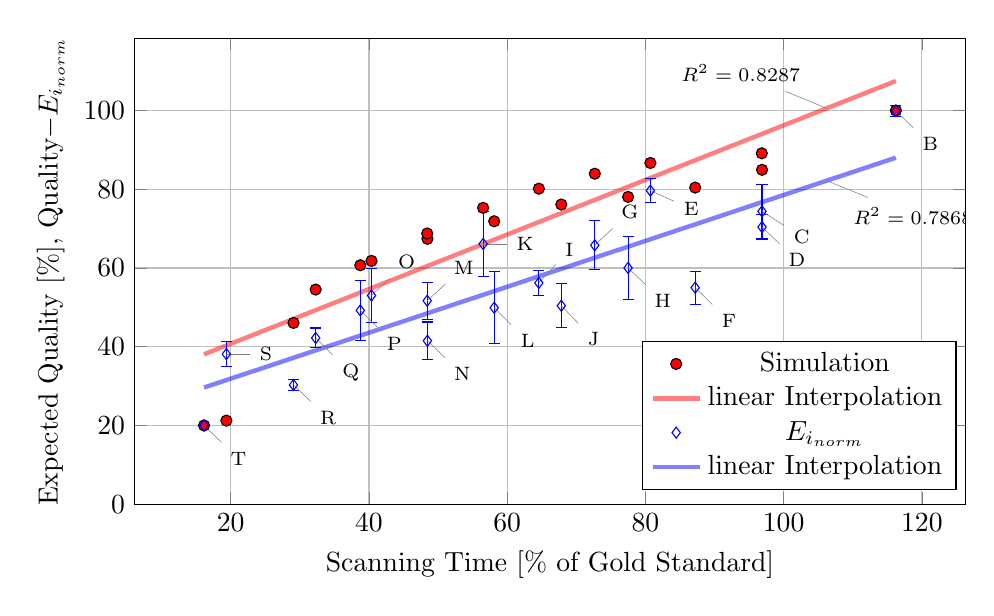
\begin{tikzpicture}

\pgfplotsset{every axis legend/.append style={at={(0.8,0.08)},anchor=base}}

\begin{axis}[%
	xmajorgrids,
  ymajorgrids,
	width=\linewidth,
	height=0.618\linewidth,
	%scale only axis,
	%xmin=0,%xmax=129,
	ymin=0,%ymax=125,
  xlabel={Scanning Time [\%\ of Gold Standard]},%
	ylabel={Expected Quality [\%], Quality$-E_{i_{norm}}$}%
	]

% Protocols
\addplot [ fill=red, only marks, mark = *]
	coordinates{
		(16.14,20)
		(19.37,21.2284)
		(29.08,46.0522)
		(32.29,54.5201)
		(38.75,60.7072)
		(40.37,61.8107)
		(48.46,67.4167)
		(48.43,68.7811)
		(58.12,71.8724)
		(56.52,75.28)
		(67.83,76.1345)
		(64.58,80.1592)
		(77.49,78.0612)
		(72.67,83.9645)
		(87.20,80.4284)
		(80.72,86.6889)
		(96.87,84.9458)
		(96.84,89.1421)
		(116.24,100)
};

\addplot [domain=16.14:116.24,color=red, semitransparent,ultra thick]
	{0.6936*x+26.891}; 

%% Line plot
%\addplot [smooth, solid, semitransparent]
	%coordinates{
		%(16.14,16.8548)
		%(19.37,25.9575)
		%(29.08,46.6567)
		%(32.29,51.7347)
		%(38.75,59.9714)
		%(40.37,61.6854) 
		%(48.46,68.6146)
		%(48.43,68.6305) 
		%(56.52,73.5452)
		%(58.12,74.3455)
		%(64.58,77.1605)
		%(67.83,78.3754)
		%(72.67,80.0091)
		%(77.49,81.5005)
		%(80.72,82.4599)
		%(87.20,84.3973)
		%(96.87,87.719)
%%		(96.87,87.719)
		%(116.24,99.8565)
%};

\addplot [ color=blue, only marks, mark=diamond ]
plot [ error bars/.cd, y dir=both, y explicit ]
    coordinates{
	( 16.14,20.0000) +- (0,0)      % T
	( 19.37,38.1358) +- (0,3.1135) % S
	( 29.08,30.2919) +- (0,1.3958) % R
	( 32.29,42.2255) +- (0,2.5278) % Q
	( 38.75,49.2247) +- (0,7.6789) % P
	( 40.37,53.0181) +- (0,6.8507) % O 
	( 48.46,41.5079) +- (0,4.7824) % N  
	( 48.43,51.6990) +- (0,4.7110) % M
	( 58.12,49.9058) +- (0,9.1839) % L
	( 56.52,66.1100) +- (0,8.1635) % K
	( 67.83,50.4137) +- (0,5.5671) % J
	( 64.58,56.2138) +- (0,3.2329) % I
	( 77.49,60.0243) +- (0,8.0805) % H
	( 72.67,65.7727) +- (0,6.2214) % G
	( 87.20,55.0069) +- (0,4.1882) % F
	( 80.72,79.6708) +- (0,3.0107) % E
	( 96.87,70.4018) +- (0,3.0863) % D
	( 96.87,74.3991) +- (0,6.8125) % C
	(116.24,99.8987) +- (0,1.3487) % B
};

\addplot [domain=16.14:116.24,color=blue, semitransparent,ultra thick]
	{0.5833*x+20.226}; 

\legend{%
	Simulation,%
	linear Interpolation,%
	$E_{i_{norm}}$,%
	linear Interpolation}

% \draw [<-] (axis cs:97.87,74.3991) -- (axis cs:99.87,74.3991) node [anchor=text] {\tiny C}; 
% \draw [<-] (axis cs:97.87,70.4018) -- (axis cs:99.87,70.4018) node [anchor=text] {\tiny D};
% \draw [<-] (axis cs:81.72,79.6708) -- (axis cs:82.72,79.6708) node [anchor=text] {\tiny E};
% \draw [<-] (axis cs:78.49,60.0243) -- (axis cs:79.49,60.0243) node [anchor=text] {\tiny H};
% \draw [<-] (axis cs:65.58,56.2138) -- (axis cs:66.58,56.2138) node [anchor=text] {\tiny I};
% \draw [<-] (axis cs:49.43,51.6990) -- (axis cs:51.43,51.6990) node [anchor=text] {\tiny M};
% \draw [<-] (axis cs:49.46,41.5079) -- (axis cs:51.46,41.5079) node [anchor=text] {\tiny N};

\tikzstyle{every pin}=[pin distance=2ex,font=\scriptsize]
\node[coordinate, pin=below right:{B}] at (axis cs:116.24,99.8987) {}; % B
\node[coordinate, pin=-22.5:{C}] at (axis cs:96.87,74.3991) {}; % C
\node[coordinate, pin=below right:{D}] at (axis cs:96.87,70.4018) {}; % D
\node[coordinate, pin=-5:{E}] at (axis cs:80.72,79.6708) {}; % E
\node[coordinate, pin=below right:{F}] at (axis cs:87.20,55.0069) {}; % F
\node[coordinate, pin=above right:{G}] at (axis cs:72.67,65.7727) {}; % G
\node[coordinate, pin=below right:{H}] at (axis cs:77.49,60.0243) {}; % H
\node[coordinate, pin=above right:{I}] at (axis cs:64.58,56.2138) {}; % I
\node[coordinate, pin=below right:{J}] at (axis cs:67.83,50.4137) {}; % J
\node[coordinate, pin=right:{K}] at (axis cs:56.52,66.1100) {}; % K
\node[coordinate, pin=below right:{L}] at (axis cs:58.12,49.9058) {}; % L
\node[coordinate, pin=above right:{M}] at (axis cs:48.43,51.6990) {}; % M
\node[coordinate, pin=below right:{N}] at (axis cs:48.46,41.5079) {}; % N  
\node[coordinate, pin=above right:{O}] at (axis cs:40.37,53.0181) {}; % O
\node[coordinate, pin=below right:{P}] at (axis cs:38.75,49.2247) {}; % P
\node[coordinate, pin=below right:{Q}] at (axis cs:32.29,42.2255) {}; % Q
\node[coordinate, pin=below right:{R}] at (axis cs:29.08,30.2919) {}; % R
\node[coordinate, pin=right:{S}] at (axis cs:19.37,38.1358) {}; % S
\node[coordinate, pin=below right:{T}] at (axis cs:16.14,20.0000) {}; % T

\node[coordinate, pin=above left:{$R^2=0.8287$}] at (axis cs:106.24,100.5791) {};
\node[coordinate, pin=below right:{$R^2=0.7868$}] at (axis cs:106.24, 82.1958) {};


\end{axis}

\end{tikzpicture}
%%%%%%%%%%%%%%%%%%%%%%%%%%%%%%
%\end{preview}
%\end{document}

%%%%%%%%%%%%%%%%%%%%%%%%%%%%%%
% plot erstellt mit MATLAB-File p:\\MATLAB\WideFieldScan/Paper/wfs_Compare2008c_ErrorPlot.m
% mit FromToTo = 1:5:1024
% sowie matlab2tikz
% Daten
%%%%%%%%%%Time =
%%%%%%%%%%  Columns 1 through 12
%%%%%%%%%%
%%%%%%%%%%   13.75   16.50   24.77   27.50   33   34.38   41.27   41.25   49.50   48.14   57.77   55
%%%%%%%%%%
%%%%%%%%%%  Columns 13 through 19
%%%%%%%%%%
%%%%%%%%%%   66   61.89   74.27   68.75   82.50   82.50   99.01
%MeanCumulativeError =
%
%  Columns 1 through 12
%
%   20.0000   38.1358   30.2919   42.2255   49.2247   53.0181   41.5079   51.6990   49.9058   66.1100   50.4137   56.2138
%
%  Columns 13 through 19
%
%   60.0243   65.7727   55.0069   79.6708   70.4018   74.3991   99.8987
%
%
%StandardDeviationofCumulativeError =
%
%  Columns 1 through 12
%
%         0    3.1135    1.3958    2.5278    7.6789    6.8507    4.7824    4.7110    9.1839    8.1635    5.5671    3.2329
%
%  Columns 13 through 19
%
%    8.0805    6.2214    4.1882    3.0107    3.0863    6.8125    1.3487
%%%%%%%%%%%%%%%%%%%%%%%%%%%%%%%
		\label{fig:NormalizedErrorPlot}%
	\end{figure}%
\else
	\begin{figure}[htp]
		\centering
		%\documentclass{article}
%\usepackage{tikz,pgfplots}
%\usepackage[pdftex,active,tightpage]{preview}
%\begin{document}
%\begin{preview}
%%%%%%%%%%%%%%%%%%%%%%%%%%%%%%
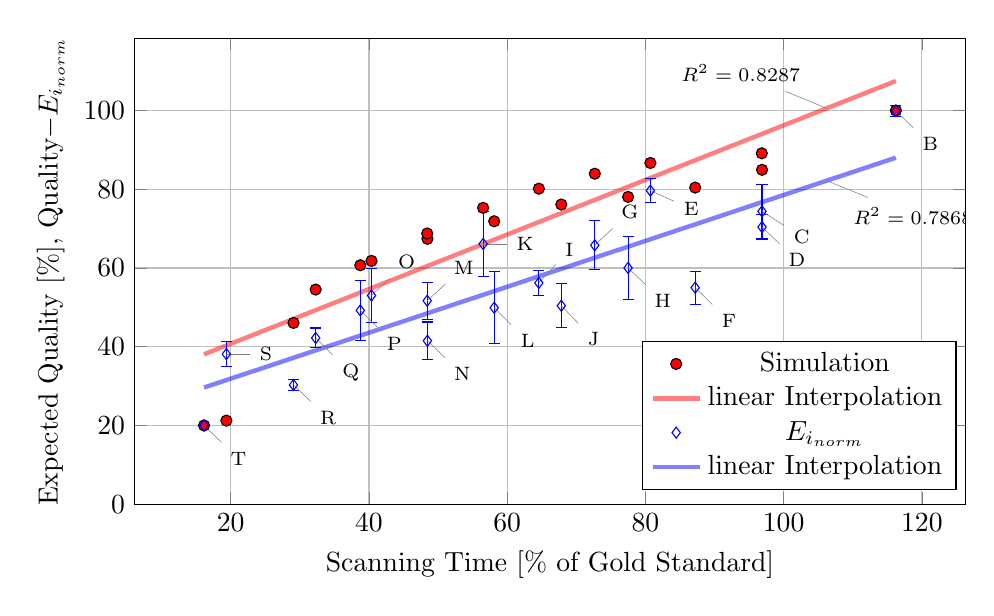
\begin{tikzpicture}

\pgfplotsset{every axis legend/.append style={at={(0.8,0.08)},anchor=base}}

\begin{axis}[%
	xmajorgrids,
  ymajorgrids,
	width=\linewidth,
	height=0.618\linewidth,
	%scale only axis,
	%xmin=0,%xmax=129,
	ymin=0,%ymax=125,
  xlabel={Scanning Time [\%\ of Gold Standard]},%
	ylabel={Expected Quality [\%], Quality$-E_{i_{norm}}$}%
	]

% Protocols
\addplot [ fill=red, only marks, mark = *]
	coordinates{
		(16.14,20)
		(19.37,21.2284)
		(29.08,46.0522)
		(32.29,54.5201)
		(38.75,60.7072)
		(40.37,61.8107)
		(48.46,67.4167)
		(48.43,68.7811)
		(58.12,71.8724)
		(56.52,75.28)
		(67.83,76.1345)
		(64.58,80.1592)
		(77.49,78.0612)
		(72.67,83.9645)
		(87.20,80.4284)
		(80.72,86.6889)
		(96.87,84.9458)
		(96.84,89.1421)
		(116.24,100)
};

\addplot [domain=16.14:116.24,color=red, semitransparent,ultra thick]
	{0.6936*x+26.891}; 

%% Line plot
%\addplot [smooth, solid, semitransparent]
	%coordinates{
		%(16.14,16.8548)
		%(19.37,25.9575)
		%(29.08,46.6567)
		%(32.29,51.7347)
		%(38.75,59.9714)
		%(40.37,61.6854) 
		%(48.46,68.6146)
		%(48.43,68.6305) 
		%(56.52,73.5452)
		%(58.12,74.3455)
		%(64.58,77.1605)
		%(67.83,78.3754)
		%(72.67,80.0091)
		%(77.49,81.5005)
		%(80.72,82.4599)
		%(87.20,84.3973)
		%(96.87,87.719)
%%		(96.87,87.719)
		%(116.24,99.8565)
%};

\addplot [ color=blue, only marks, mark=diamond ]
plot [ error bars/.cd, y dir=both, y explicit ]
    coordinates{
	( 16.14,20.0000) +- (0,0)      % T
	( 19.37,38.1358) +- (0,3.1135) % S
	( 29.08,30.2919) +- (0,1.3958) % R
	( 32.29,42.2255) +- (0,2.5278) % Q
	( 38.75,49.2247) +- (0,7.6789) % P
	( 40.37,53.0181) +- (0,6.8507) % O 
	( 48.46,41.5079) +- (0,4.7824) % N  
	( 48.43,51.6990) +- (0,4.7110) % M
	( 58.12,49.9058) +- (0,9.1839) % L
	( 56.52,66.1100) +- (0,8.1635) % K
	( 67.83,50.4137) +- (0,5.5671) % J
	( 64.58,56.2138) +- (0,3.2329) % I
	( 77.49,60.0243) +- (0,8.0805) % H
	( 72.67,65.7727) +- (0,6.2214) % G
	( 87.20,55.0069) +- (0,4.1882) % F
	( 80.72,79.6708) +- (0,3.0107) % E
	( 96.87,70.4018) +- (0,3.0863) % D
	( 96.87,74.3991) +- (0,6.8125) % C
	(116.24,99.8987) +- (0,1.3487) % B
};

\addplot [domain=16.14:116.24,color=blue, semitransparent,ultra thick]
	{0.5833*x+20.226}; 

\legend{%
	Simulation,%
	linear Interpolation,%
	$E_{i_{norm}}$,%
	linear Interpolation}

% \draw [<-] (axis cs:97.87,74.3991) -- (axis cs:99.87,74.3991) node [anchor=text] {\tiny C}; 
% \draw [<-] (axis cs:97.87,70.4018) -- (axis cs:99.87,70.4018) node [anchor=text] {\tiny D};
% \draw [<-] (axis cs:81.72,79.6708) -- (axis cs:82.72,79.6708) node [anchor=text] {\tiny E};
% \draw [<-] (axis cs:78.49,60.0243) -- (axis cs:79.49,60.0243) node [anchor=text] {\tiny H};
% \draw [<-] (axis cs:65.58,56.2138) -- (axis cs:66.58,56.2138) node [anchor=text] {\tiny I};
% \draw [<-] (axis cs:49.43,51.6990) -- (axis cs:51.43,51.6990) node [anchor=text] {\tiny M};
% \draw [<-] (axis cs:49.46,41.5079) -- (axis cs:51.46,41.5079) node [anchor=text] {\tiny N};

\tikzstyle{every pin}=[pin distance=2ex,font=\scriptsize]
\node[coordinate, pin=below right:{B}] at (axis cs:116.24,99.8987) {}; % B
\node[coordinate, pin=-22.5:{C}] at (axis cs:96.87,74.3991) {}; % C
\node[coordinate, pin=below right:{D}] at (axis cs:96.87,70.4018) {}; % D
\node[coordinate, pin=-5:{E}] at (axis cs:80.72,79.6708) {}; % E
\node[coordinate, pin=below right:{F}] at (axis cs:87.20,55.0069) {}; % F
\node[coordinate, pin=above right:{G}] at (axis cs:72.67,65.7727) {}; % G
\node[coordinate, pin=below right:{H}] at (axis cs:77.49,60.0243) {}; % H
\node[coordinate, pin=above right:{I}] at (axis cs:64.58,56.2138) {}; % I
\node[coordinate, pin=below right:{J}] at (axis cs:67.83,50.4137) {}; % J
\node[coordinate, pin=right:{K}] at (axis cs:56.52,66.1100) {}; % K
\node[coordinate, pin=below right:{L}] at (axis cs:58.12,49.9058) {}; % L
\node[coordinate, pin=above right:{M}] at (axis cs:48.43,51.6990) {}; % M
\node[coordinate, pin=below right:{N}] at (axis cs:48.46,41.5079) {}; % N  
\node[coordinate, pin=above right:{O}] at (axis cs:40.37,53.0181) {}; % O
\node[coordinate, pin=below right:{P}] at (axis cs:38.75,49.2247) {}; % P
\node[coordinate, pin=below right:{Q}] at (axis cs:32.29,42.2255) {}; % Q
\node[coordinate, pin=below right:{R}] at (axis cs:29.08,30.2919) {}; % R
\node[coordinate, pin=right:{S}] at (axis cs:19.37,38.1358) {}; % S
\node[coordinate, pin=below right:{T}] at (axis cs:16.14,20.0000) {}; % T

\node[coordinate, pin=above left:{$R^2=0.8287$}] at (axis cs:106.24,100.5791) {};
\node[coordinate, pin=below right:{$R^2=0.7868$}] at (axis cs:106.24, 82.1958) {};


\end{axis}

\end{tikzpicture}
%%%%%%%%%%%%%%%%%%%%%%%%%%%%%%
%\end{preview}
%\end{document}

%%%%%%%%%%%%%%%%%%%%%%%%%%%%%%
% plot erstellt mit MATLAB-File p:\\MATLAB\WideFieldScan/Paper/wfs_Compare2008c_ErrorPlot.m
% mit FromToTo = 1:5:1024
% sowie matlab2tikz
% Daten
%%%%%%%%%%Time =
%%%%%%%%%%  Columns 1 through 12
%%%%%%%%%%
%%%%%%%%%%   13.75   16.50   24.77   27.50   33   34.38   41.27   41.25   49.50   48.14   57.77   55
%%%%%%%%%%
%%%%%%%%%%  Columns 13 through 19
%%%%%%%%%%
%%%%%%%%%%   66   61.89   74.27   68.75   82.50   82.50   99.01
%MeanCumulativeError =
%
%  Columns 1 through 12
%
%   20.0000   38.1358   30.2919   42.2255   49.2247   53.0181   41.5079   51.6990   49.9058   66.1100   50.4137   56.2138
%
%  Columns 13 through 19
%
%   60.0243   65.7727   55.0069   79.6708   70.4018   74.3991   99.8987
%
%
%StandardDeviationofCumulativeError =
%
%  Columns 1 through 12
%
%         0    3.1135    1.3958    2.5278    7.6789    6.8507    4.7824    4.7110    9.1839    8.1635    5.5671    3.2329
%
%  Columns 13 through 19
%
%    8.0805    6.2214    4.1882    3.0107    3.0863    6.8125    1.3487
%%%%%%%%%%%%%%%%%%%%%%%%%%%%%%
		\caption{%
			Plot of normalized difference Value ($E_{i_{norm}}$, blue diamonds) for the 19 scanned protocols overlaid over Quality-plot (red dots) obtained from the simulation. The normalized Error has been calculated using the difference image of each protocol $i$ with protocol B. The error bars for each protocol show the standard deviation of the error calculated for 205 of the 1024 slices. Note that the scale of the error was normalized to 20--\SI{100}{\percent}, so that both the quality from the simulation and the error are directly comparable. The abscissa shows the scanning time in percentage of time used for the gold standard scan. Protocol T corresponds to the fastest scanning time, protocol B to the slowest. The protocols in between are shown in decreasing order from T--B for increasing percentage of the scanning time.%
		}%
		\label{fig:NormalizedErrorPlot}
	\end{figure}
\fi

\subsubsection{three-dimensional visualization of different protocols}
\label{subsec:comparison}
x	The tomograms of the different protocols were three-dimensionally analyzed and visualized using MeVisLab (Version 2.0 (2009-06-09 Release), MeVis Medical Solutions AG and Fraunhofer MEVIS - Institute for Medical Image Computing, Bremen, Germany). Airway segments were extracted using a threshold interval based region growing algorithm. A seed point for the region growing algorithm was manually defined in the most proximal slice for each independent airway segment. The coordinates of the seed points were kept constant for protocol B--T, allowing direct comparison between the airway segment reconstructions of the different protocols. Airway segments extracted for protocol B, L and T are shown in figure~\ref{fig:BvsT}.

The data shown in figure~\ref{fig:BvsT} represent three of the 19 scanned protocols. Protocol B corresponds to a slightly oversampled gold standard scan, obtained with 15732 projections for all three subscans, recorded in \SI{66}{\minute}. Protocol L was obtained in \SI{35}{\minute} with total 7866 projections. Protocol T was obtained in \SI{12}{\minute} with total 2185 projections. The tomographic dataset from protocol B was reconstructed from 5244 merged projection images, the dataset from protocol L was reconstructed from 2622 merged projections and the dataset from protocol T was reconstructed using only 874 merged projections. Even though protocols L and T were scanned while violating the sampling theorem and with a total scanning time reduction of \SI{40}{\percent} (or more than \SI{86}{\percent}), the samples still appear to be identical to the gold standard protocol in the low-resolution three-dimensional visualization, as shown in figure~\ref{fig:BvsT}(a), (b) and (c).

Obviously, the artifacts introduced through the reduction in scanning time only become apparent at higher magnification. The blue cube inside the green airway segments in figures~\ref{fig:BvsT}(a), (b) and (c) are shown as isosurface visualizations of the lung tissue (which corresponds exactly to the negative of the extracted airway segment) in figures~\ref{fig:BvsT}(d), (e) and (f). The regions of interest show a cube with a side length of \SI{379}{\micro\meter} or 256 pixels.

Even with the higher magnification, the reconstruction of protocol L in figure~\ref{fig:BvsT}(e) appears nearly identical to the reconstruction of the region of interest of protocol B (fig.~\ref{fig:BvsT}(d)). The isosurface of the region of interest of protocol T shown in figure~\ref{fig:BvsT}(f) appears rougher than the isosurface of protocol B. This roughness is introduced through wave-like artifacts visible in the original slice of the dataset of protocol T (not shown). These artifacts arise through the breaching of the sampling theorem, since only 874 projections were acquired for the two ring-scans instead of the 5139 projections ($(3072-200)\frac{\pi}{2}$) required to satisfy the sampling theorem. However, even with this strong undersampling, segmentation, three-dimensional reconstruction and visualization of the sample is still possible.

\ifiucr%%% iucr %%%
%\onecolumn
	\begin{figure}
		\caption{%
			Comparison of three-dimensional visualizations of protocols B, L and T. %
			(a) Three independent airway segments (green, red, yellow) of Protocol B were extracted using a region growing algorithm. %
			(b) Same for protocol L. %
			(c) Same for protocol T. A cubical region of interest (ROI, blue) with a side length of 256 pixels (corresponding to \SI{379}{\micro\meter}) is marked inside the leftmost segment for all protocols. %
			(d): Detailed view of isosurfaces of the lung tissue inside the ROIs shown for protocol B. %
			(e): Same for protocol L.
			(f): Same for protocol T. Note the artifacts in the isosurface in subfigure (e) and (f).%
			}%
		\renewcommand{\imsize}{.33\linewidth}%
		\pgfmathsetlength{\imagewidth}{\imsize}%
		\pgfmathsetlength{\imagescale}{\imagewidth/1085}%
		\def\x{551} % scalebar-x at golden ratio of x=1085px (671px = golden ratio: 551 is set to fit the one-column-width in the draft mode!!!)
		\def\y{530} % scalebar-y at 90% of height of y=589px
		\begin{tikzpicture}[x=\imagescale,y=-\imagescale]
			\node[anchor=north west, inner sep=0pt, outer sep=0pt] at (0,0)
				{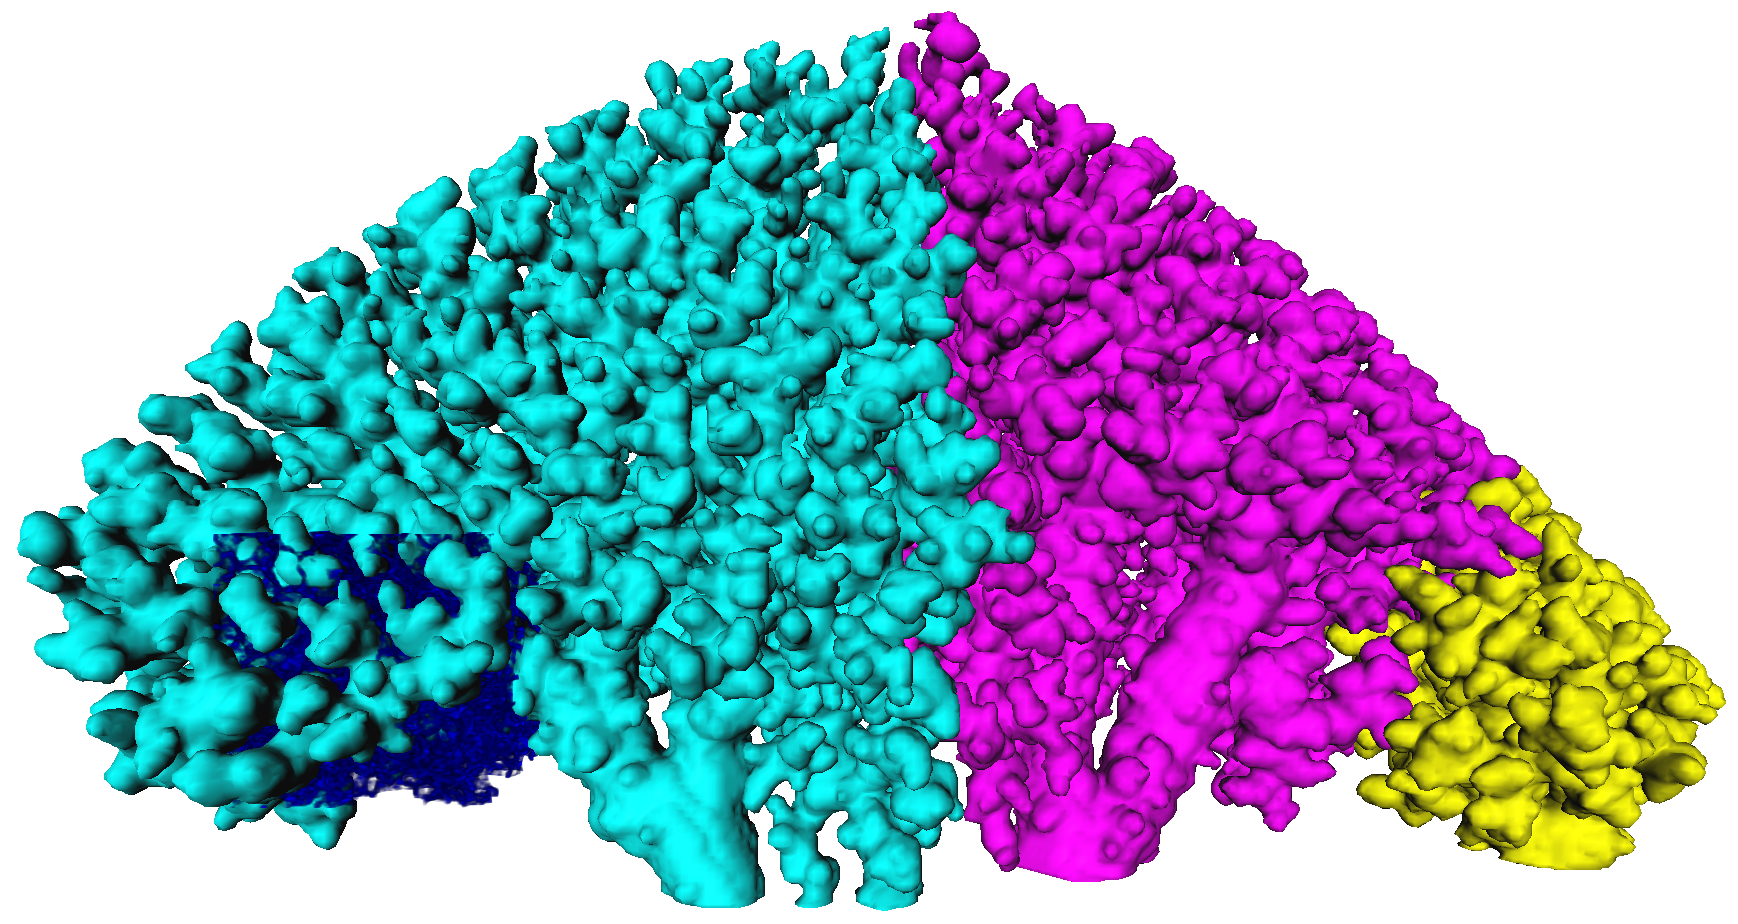
\includegraphics[width=\imagewidth]{img/comparisonBvsT/ob}};
			% 1030px = 2.627mm > 100px = 255um > 196px = 500um
%			\draw[|-|,thick] (30,339) -- (1054,454) node [white,sloped,midway,above] {\SI{2.627}{\milli\meter} (1775px)};
			\draw [|-|,thick] (\x,\y) -- (\x+196,\y) node [fill=white,semitransparent,right] {\SI{500}{\micro\meter}} node [right] {\SI{500}{\micro\meter}};
			\node [fill=white,semitransparent,anchor=south west] at (0,589) {(a)};
			\node [anchor=south west] at (0,589) {(a)};
		\end{tikzpicture}%
		\begin{tikzpicture}[x=\imagescale,y=-\imagescale]%
			\node[anchor=north west, inner sep=0pt, outer sep=0pt] at (0,0)
				{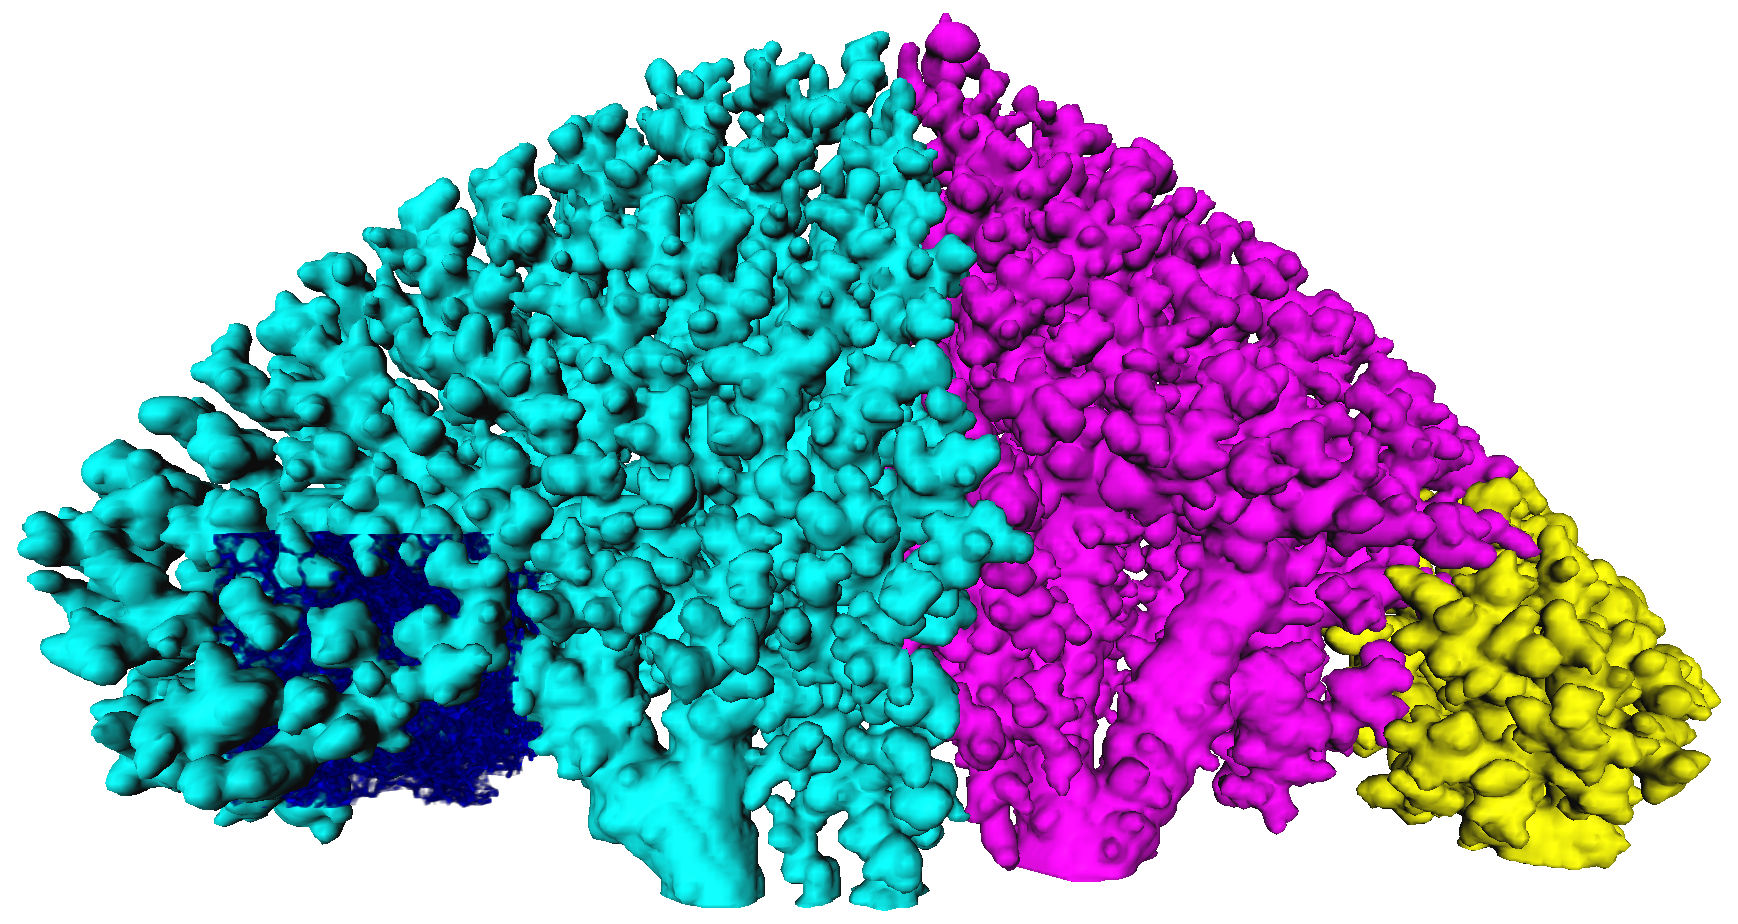
\includegraphics[width=\imagewidth]{img/comparisonBvsT/ol}};
			% 1030px = 2.627mm > 100px = 255um > 196px = 500um
			\draw [|-|,thick] (\x,\y) -- (\x+196,\y) node [fill=white,semitransparent,right] {\SI{500}{\micro\meter}} node [right] {\SI{500}{\micro\meter}};
			\node [fill=white,semitransparent,anchor=south west] at (0,589) {(b)};
			\node [anchor=south west] at (0,589) {(b)};
		\end{tikzpicture}%
		\begin{tikzpicture}[x=\imagescale,y=-\imagescale]%
			\node[anchor=north west, inner sep=0pt, outer sep=0pt] at (0,0)
				{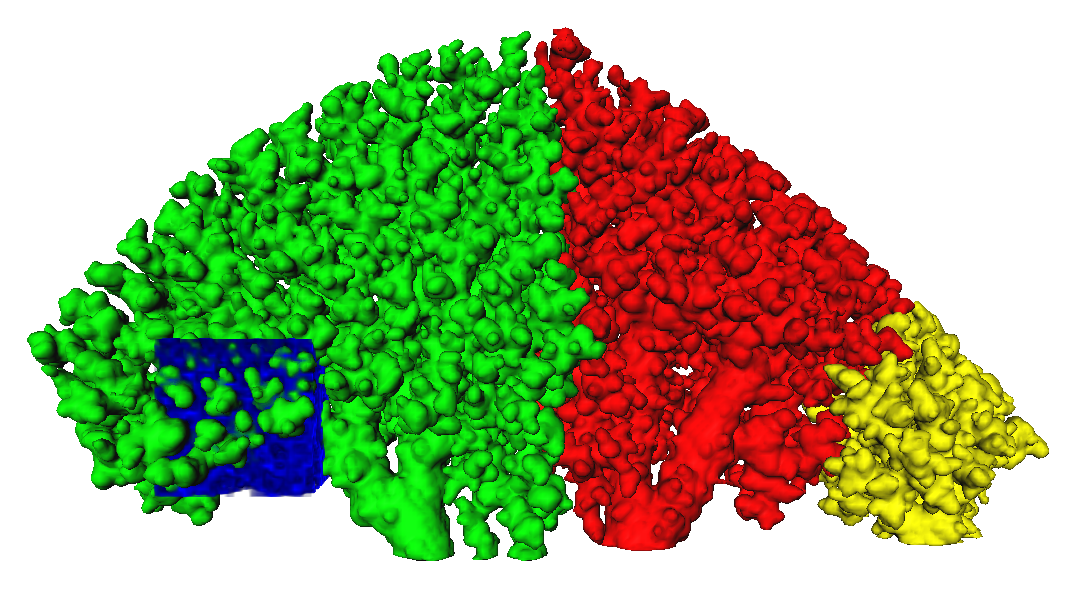
\includegraphics[width=\imagewidth]{img/comparisonBvsT/ot}};
			% 1030px = 2.627mm > 100px = 255um > 196px = 500um
			\draw [|-|,thick] (\x,\y) -- (\x+196,\y) node [fill=white,semitransparent,right] {\SI{500}{\micro\meter}} node [right] {\SI{500}{\micro\meter}};
			\node [fill=white,semitransparent,anchor=south west] at (0,589) {(c)};
			\node [anchor=south west] at (0,589) {(c)};
		\end{tikzpicture}%
		\\%
		\pgfmathsetlength{\imagewidth}{\imsize}%
		\pgfmathsetlength{\imagescale}{\imagewidth/816}%
		\def\x{504} % scalebar-x at golden ratio of x=816px
		\def\y{734} % scalebar-y at 90% of height of y=815px
		\begin{tikzpicture}[x=\imagescale,y=-\imagescale]%
			\node[anchor=north west, inner sep=0pt, outer sep=0pt] at (0,0)
				{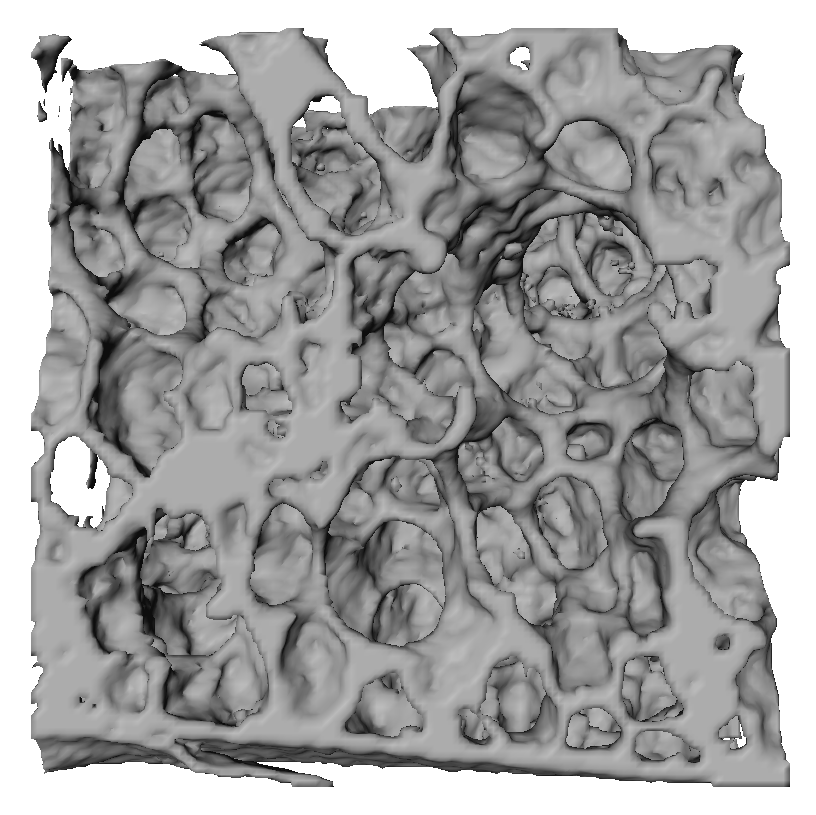
\includegraphics[width=\imagewidth]{img/comparisonBvsT/roiB}};
			% 761px = 0.37888mm > 100px = 50um > 100.4px = 500um
%			\draw[|-|,thick] (792,438) -- (31,435) node [sloped,midway,above] {\SI{378.88}{\micro\meter} (256px)};
			\draw[|-|,thick] (\x,\y) -- (\x+100.4,\y) node [fill=white,semitransparent,right] {\SI{50}{\micro\meter}} node [right] {\SI{50}{\micro\meter}};
			\node [fill=white,semitransparent,anchor=south west] at (0,815) {(d)};
			\node [anchor=south west] at (0,815) {(d)};
	\end{tikzpicture}%
		\begin{tikzpicture}[x=\imagescale,y=-\imagescale]%
			\node[anchor=north west, inner sep=0pt, outer sep=0pt] at (0,0)
				{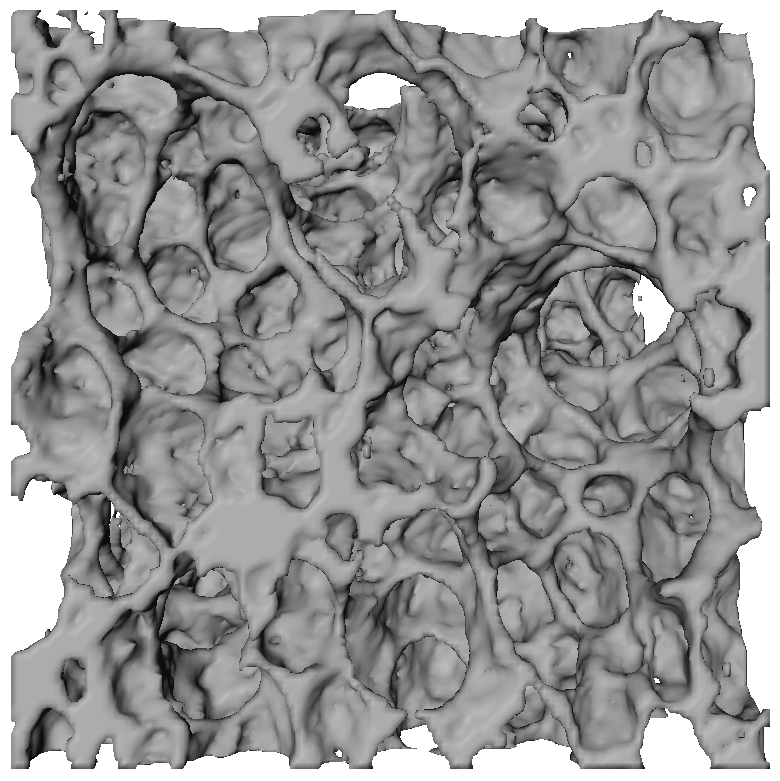
\includegraphics[width=\imagewidth]{img/comparisonBvsT/roiL}};
			% 761px = 0.37888mm > 100px = 50um > 100.4px = 500um
			\draw[|-|,thick] (\x,\y) -- (\x+100.4,\y) node [fill=white,semitransparent,right] {\SI{50}{\micro\meter}} node [right] {\SI{50}{\micro\meter}};
			\node [fill=white,semitransparent,anchor=south west] at (0,815) {(e)};
			\node [anchor=south west] at (0,815) {(e)};
		\end{tikzpicture}%
		\begin{tikzpicture}[x=\imagescale,y=-\imagescale]%
			\node[anchor=north west, inner sep=0pt, outer sep=0pt] at (0,0)
				{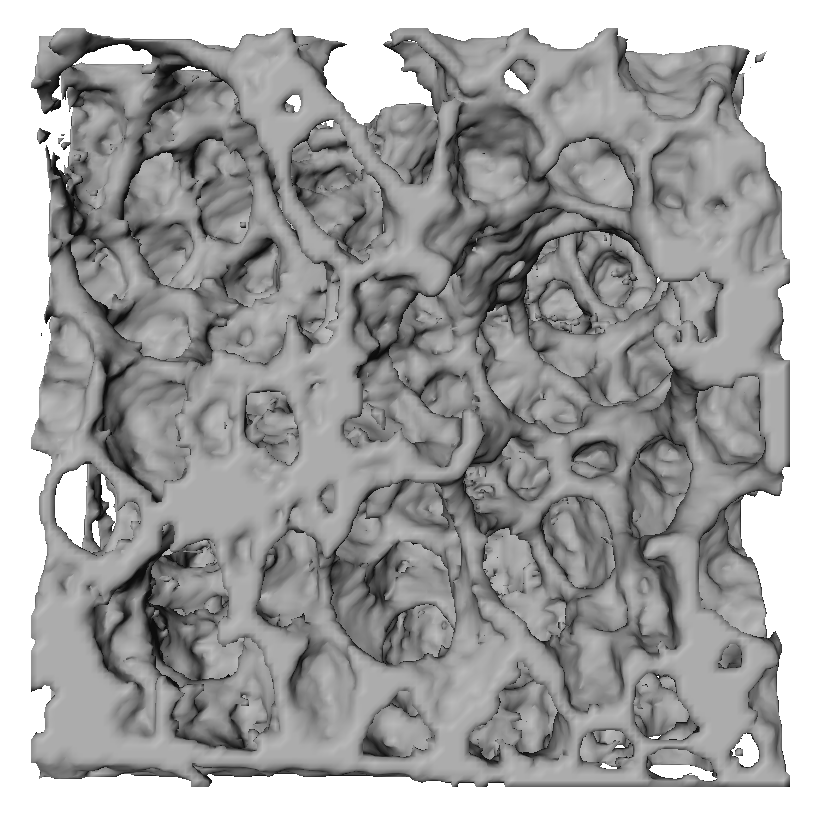
\includegraphics[width=\imagewidth]{img/comparisonBvsT/roiT}};
			% 761px = 0.37888mm > 100px = 50um > 100.4px = 500um
			\draw[|-|,thick] (\x,\y) -- (\x+100.4,\y) node [fill=white,semitransparent,right] {\SI{50}{\micro\meter}} node [right] {\SI{50}{\micro\meter}};
			\node [fill=white,semitransparent,anchor=south west] at (0,815) {(f)};
			\node [anchor=south west] at (0,815) {(f)};
		\end{tikzpicture}%
		\label{fig:BvsT}%
	\end{figure}%
%\twocolumn%
\else%
	\begin{figure}[htp]
		\centering
		\renewcommand{\imsize}{.333\linewidth}%
		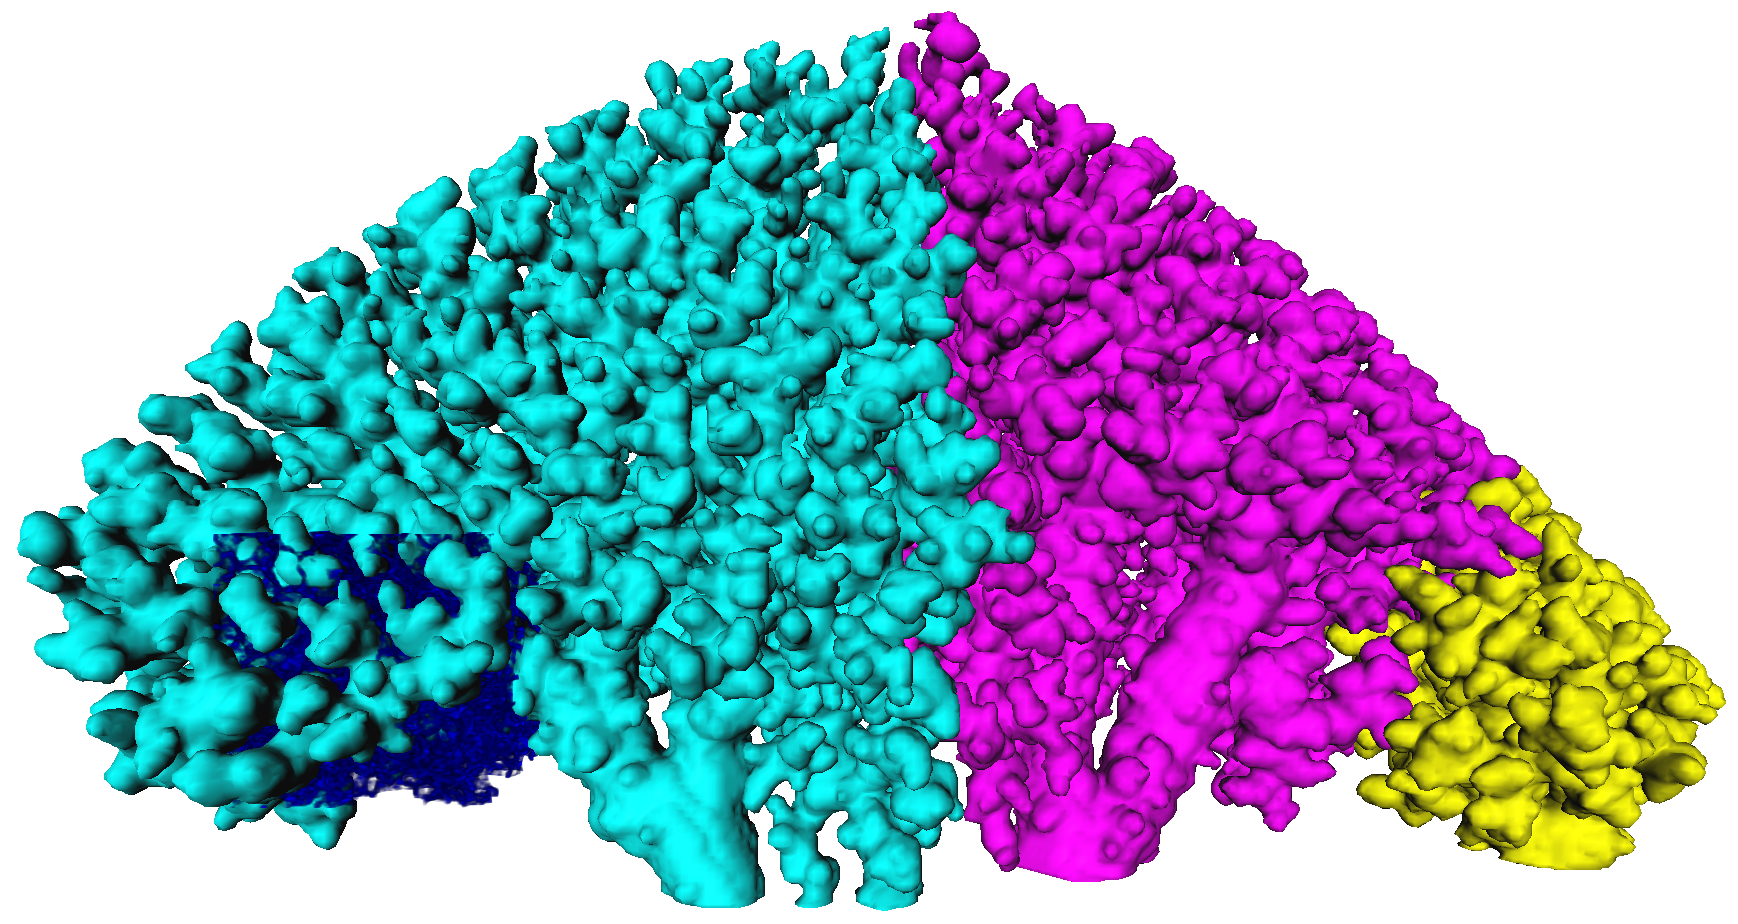
\includegraphics[width=\imagewidth]{img/comparisonBvsT/ob}%
		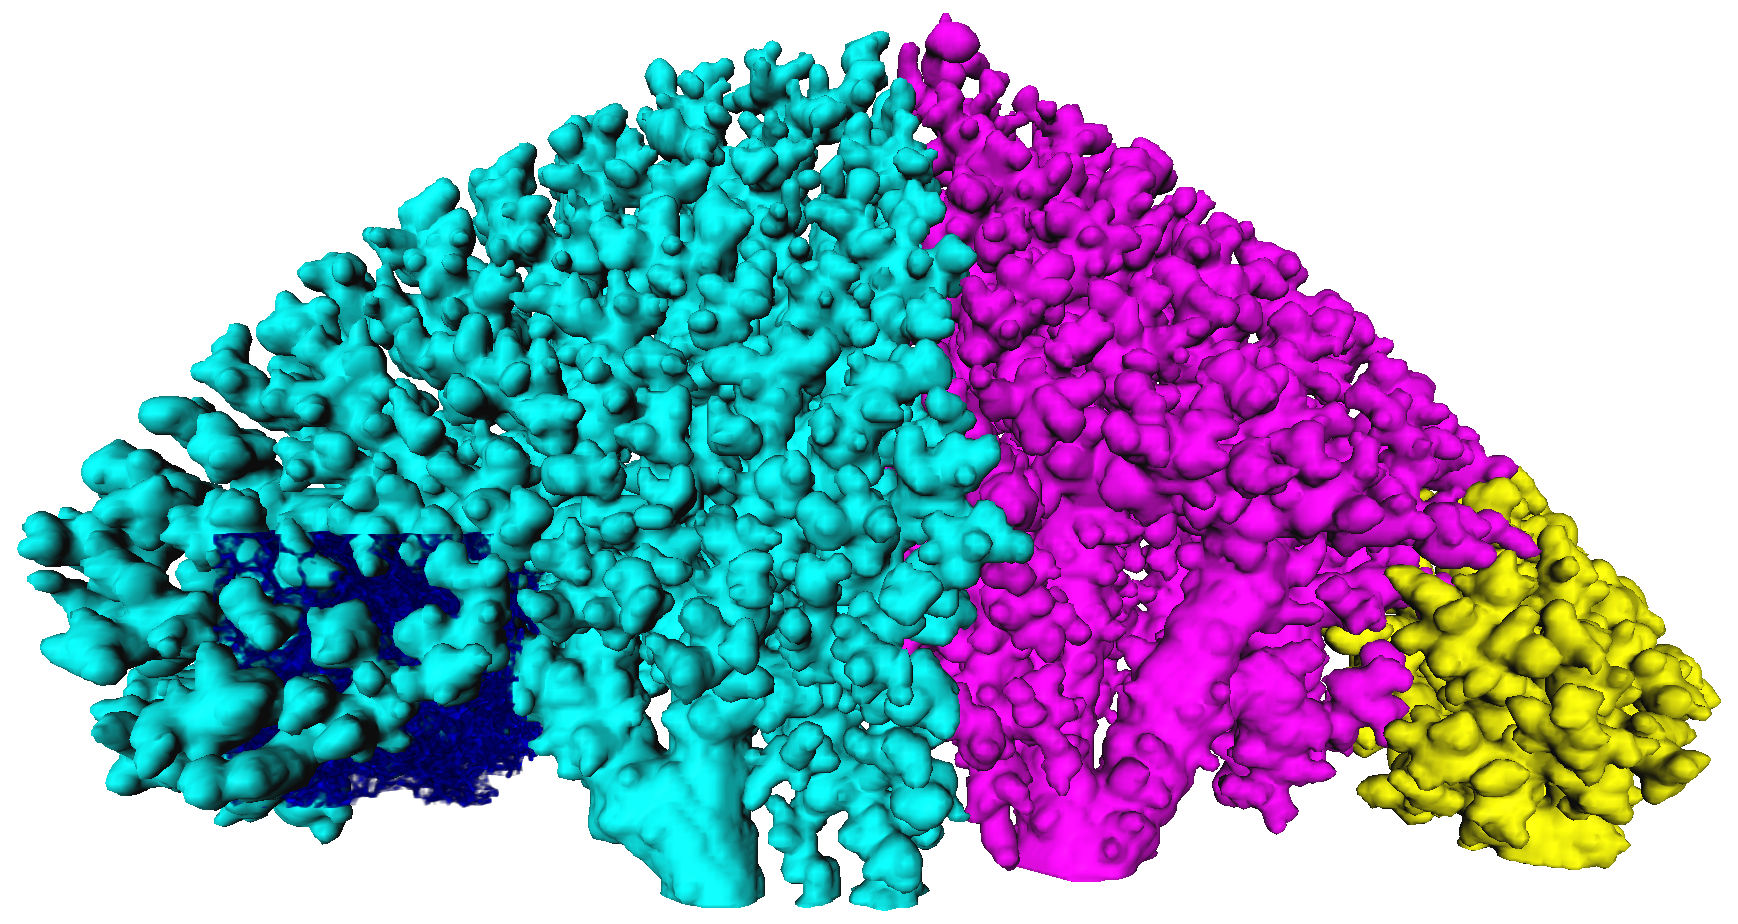
\includegraphics[width=\imagewidth]{img/comparisonBvsT/ol}%
		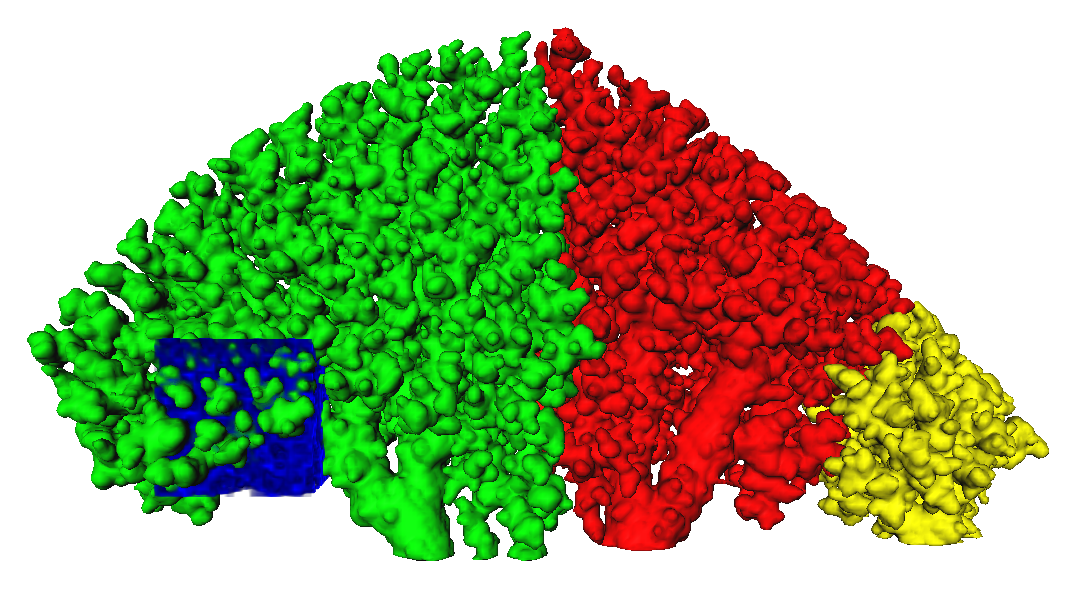
\includegraphics[width=\imagewidth]{img/comparisonBvsT/ot}%
		\\%
		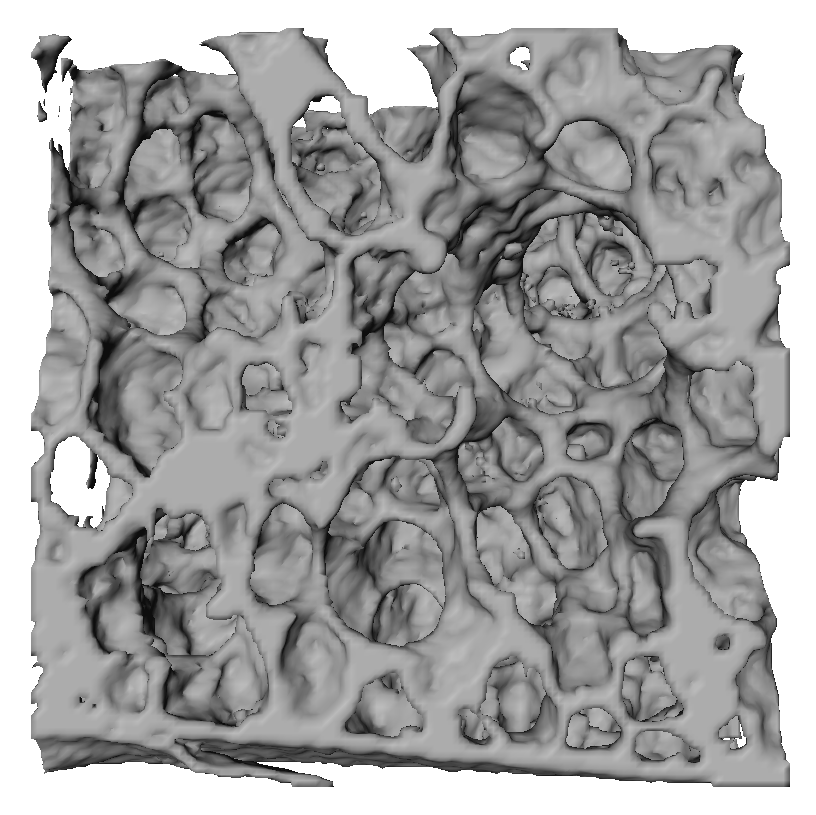
\includegraphics[width=\imagewidth]{img/comparisonBvsT/roiB}%
		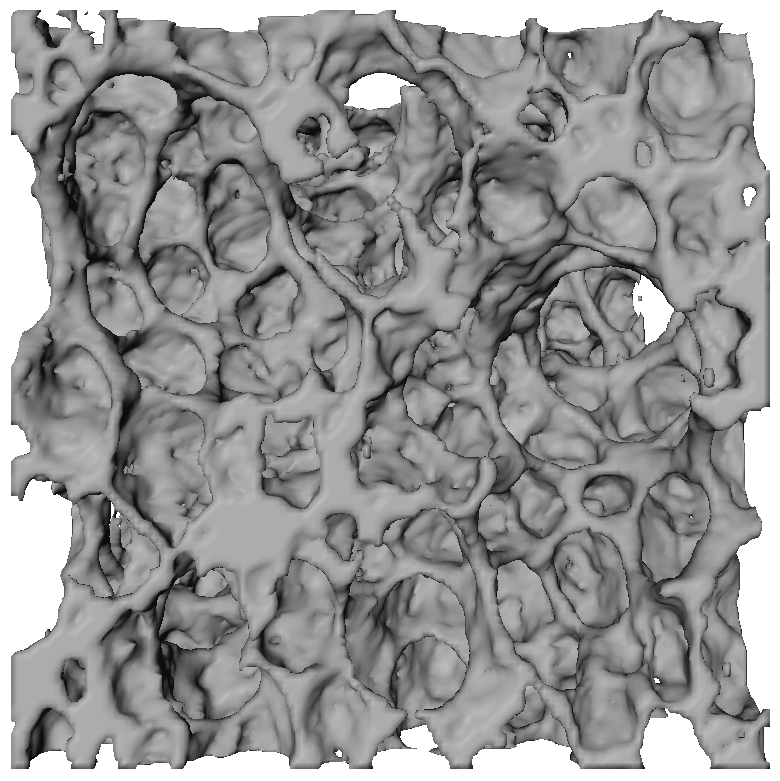
\includegraphics[width=\imagewidth]{img/comparisonBvsT/roiL}%
		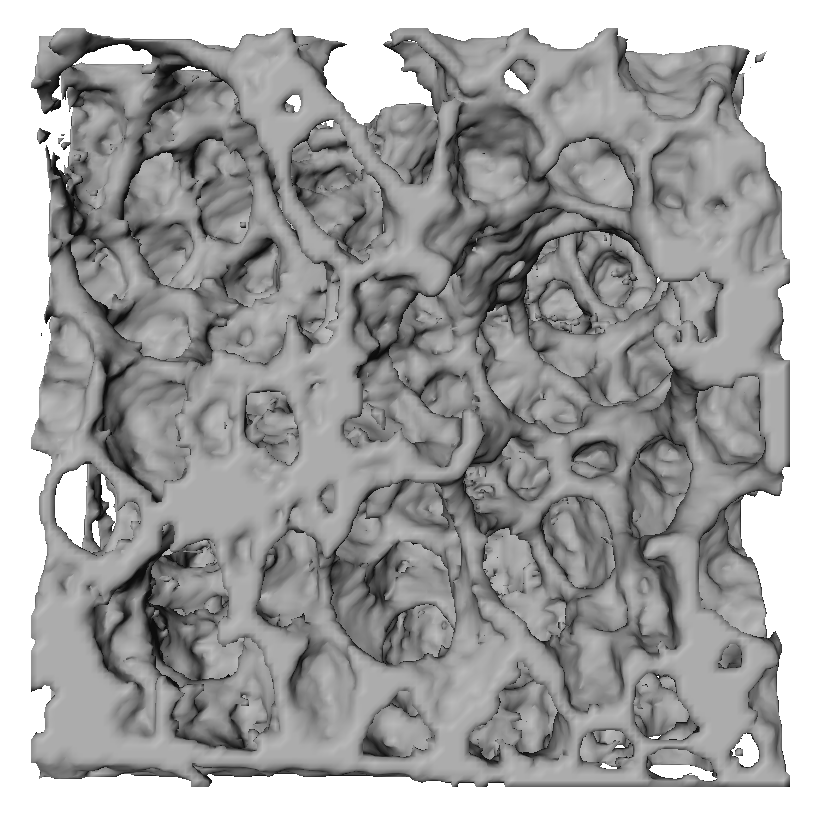
\includegraphics[width=\imagewidth]{img/comparisonBvsT/roiT}%
		\caption{%
			Comparison of three-dimensional visualizations of protocols B, L and T. %
			(a) Three independent airway segments (green, red, yellow) of Protocol B were extracted using a region growing algorithm. %
			(b) Same for protocol L. %
			(c) Same for protocol T. A cubical region of interest (ROI, blue) with a side length of 256 pixels (corresponding to \SI{379}{\micro\meter}) is marked inside the leftmost segment for all protocols. %
			(d): Detailed view of isosurfaces of the lung tissue inside the ROIs shown for protocol B. %
			(e): Same for protocol L.
			(f): Same for protocol T. Note the artifacts in the isosurface in subfigure (e) and (f).%
			}%
		\label{fig:BvsT}%
	\end{figure}
\fi%

For further analysis four regions of interest with a side length of 256 pixels (at \SI{1.48}{\micro\meter\per pixel}, thus containing a volume of \SI{1.678e7}{voxels}) have been extracted for each of the protocols B, L and T. The three-dimensional placement of these ROIs inside the sample is shown in figure~\ref{fig:roi3d}. Each of the ROIs has been binarized using an automatically determined threshold~\cite{Otsu1979} and small particles inside the segmented airspace lumen have been removed using a connected components analysis. Subsequently, the euclidean distance transformation has been calculated for each thresholded ROI.

\renewcommand{\imsize}{\columnwidth}
\begin{figure}%
	\centering%
	\pgfmathsetlength{\imagewidth}{\imsize}%
	\pgfmathsetlength{\imagescale}{\imagewidth/1452}%
	\caption{Overview of the placement of the four regions of interest where the histogram of the euclidean distance transformation distribution has been calculated. Grey: Semitransparent volume rendering of the lung tissue sample. Red: Four regions of interest, extracted to calculate the distance transformation, each with a side-length of 256 pixels. The labels of the ROIs conform to the legends in figure~\ref{fig:DTFplots}.}%
	\begin{tikzpicture}[x=\imagescale,y=-\imagescale]
		\def\x{297} % scalebar-x at golden ratio of x=1452px
		\def\y{684} % scalebar-y at 90% of height of y=760px
		\node[anchor=north west, inner sep=0pt, outer sep=0pt] at (0,0)
	     {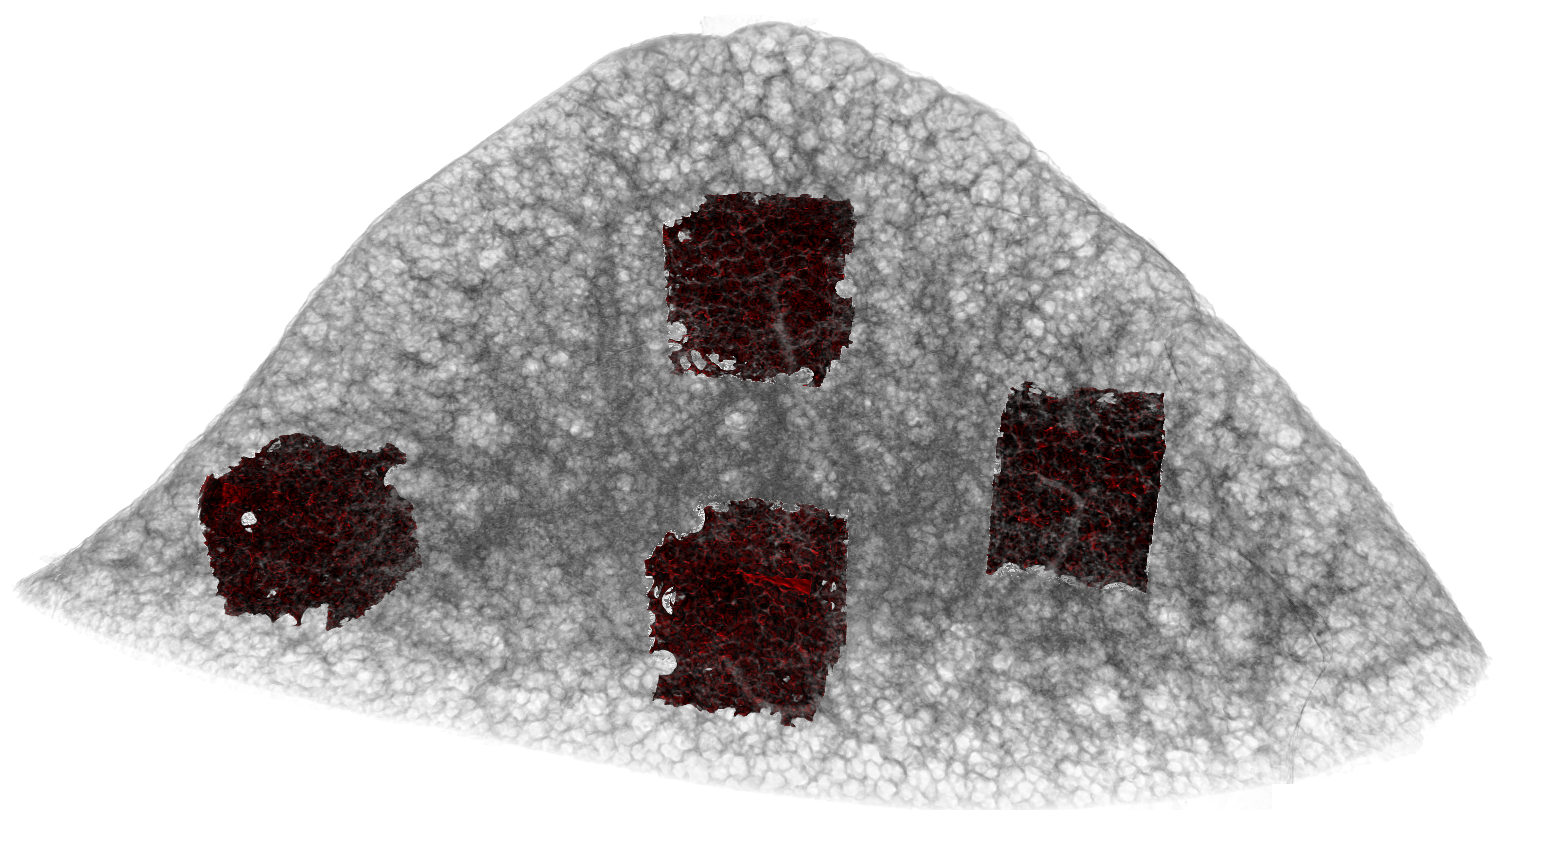
\includegraphics[width=\imagewidth]{img/dtf-roi/ROIs-3d}};
		% 1357px = 4.0138mm > 100px = 296um > 169px = 500um
		% \draw[|-|,thick,red] (83,517) -- (1425,719) node [sloped,midway,below] {\SI{4.0138}{\milli\meter} (2712px)};
		\draw[|-|,thick] (\x,\y) -- (\x+169,\y) node [midway, above] {\SI{500}{\micro\meter}};
		\draw[|-|,thick, white] (\x+645,\y-180) -- (\x+645+128,\y-180) node [midway, below] {\SI{256}{pixels}};
		\draw ( 368,360) node [fill=white, semitransparent] {ROI 1} node {ROI 1};
		\draw (1038,312) node [fill=white, semitransparent] {ROI 2} node {ROI 2};
		\draw ( 767,413) node [fill=white, semitransparent] {ROI 3} node {ROI 3};
		\draw ( 684,139) node [fill=white, semitransparent] {ROI 4} node {ROI 4};
	\end{tikzpicture}%
	\label{fig:roi3d}%
\end{figure}

For comparison, the histogram of the euclidean distance transformation has been plotted for all four regions of interest in each protocol (B, L and T).

\renewcommand{\imsize}{.309\columnwidth}
%\onecolumn
\begin{figure}%
	\centering
	\caption{Histogram-Plots for each of the of 4 ROIs, each showing the histogram of the distance transformation for the protocols B, L and T.}%		
	\begin{tabular}{cc}%
		%\documentclass{article}
%\usepackage{tikz,pgfplots}
%\usepackage[pdftex,active,tightpage]{preview}
%\begin{document}
%\begin{preview}
%%%%%%%%%%%%
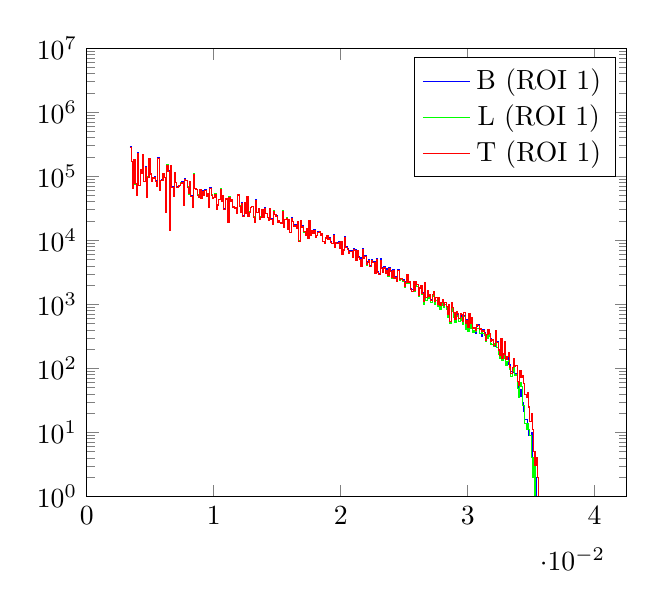
\begin{tikzpicture}

% Axis at [0.13 0.11 0.78 0.81]
\begin{semilogyaxis}[
axis on top,
xmin=0, xmax=0.0425,
ymin=1, ymax=1e+007,
%title={ROI 1},
legend entries={%
			B (ROI 1),%
			L (ROI 1),%
			T (ROI 1)}
]

\addplot [
color=blue,
solid
]coordinates{
 (0.0034,0) (0.0034,289501) (0.0034,289501) (0.0035,289501) (0.0035,168870) (0.0035,168870) (0.0036,168870) (0.0036,65511) (0.0036,65511) (0.0037,65511) (0.0037,185453) (0.0037,185453) (0.0038,185453) (0.0038,74694) (0.0038,74694) (0.0039,74694) (0.0039,52846) (0.0039,52846) (0.004,52846) (0.004,230325) (0.004,230325) (0.0041,230325) (0.0041,70838) (0.0041,70838) (0.0042,70838) (0.0042,127584) (0.0042,127584) (0.0043,127584) (0.0043,112007) (0.0043,112007) (0.0044,112007) (0.0044,220564) (0.0044,220564) (0.0045,220564) (0.0045,83095) (0.0045,83095) (0.0046,83095) (0.0046,140906) (0.0046,140906) (0.0047,140906) (0.0047,46921) (0.0047,46921) (0.0048,46921) (0.0048,98956) (0.0048,98956) (0.0049,98956) (0.0049,191119) (0.0049,191119) (0.005,191119) (0.005,109497) (0.005,109497) (0.0051,109497) (0.0051,83683) (0.0051,83683) (0.0052,83683) (0.0052,95212) (0.0052,95212) (0.0053,95212) (0.0053,98242) (0.0053,98242) (0.0054,98242) (0.0054,85358) (0.0054,85358) (0.0055,85358) (0.0055,69667) (0.0055,69667) (0.0056,69667) (0.0056,193089) (0.0056,193089) (0.0057,193089) (0.0057,60959) (0.0057,60959) (0.0058,60959) (0.0058,87206) (0.0058,87206) (0.0059,87206) (0.0059,88163) (0.0059,88163) (0.006,88163) (0.006,111357) (0.006,111357) (0.0061,111357) (0.0061,94851) (0.0061,94851) (0.0062,94851) (0.0062,28137) (0.0062,28137) (0.0063,28137) (0.0063,151541) (0.0063,151541) (0.0064,151541) (0.0064,121345) (0.0064,121345) (0.0065,121345) (0.0065,14476) (0.0065,14476) (0.0066,14476) (0.0066,148633) (0.0066,148633) (0.0067,148633) (0.0067,68210) (0.0067,68210) (0.0068,68210) (0.0068,51398) (0.0068,51398) (0.0069,51398) (0.0069,114875) (0.0069,114875) (0.007,114875) (0.007,79729) (0.007,79729) (0.0071,79729) (0.0071,68479) (0.0071,68479) (0.0072,68479) (0.0072,72250) (0.0072,72250) (0.0073,72250) (0.0073,72049) (0.0073,72049) (0.0074,72049) (0.0074,79753) (0.0074,79753) (0.0075,79753) (0.0075,81664) (0.0075,81664) (0.0076,81664) (0.0076,34829) (0.0076,34829) (0.0077,34829) (0.0077,90607) (0.0077,90607) (0.0078,90607) (0.0078,86063) (0.0078,86063) (0.0079,86063) (0.0079,69170) (0.0079,69170) (0.008,69170) (0.008,53271) (0.008,53271) (0.0081,53271) (0.0081,83343) (0.0081,83343) (0.0082,83343) (0.0082,49082) (0.0082,49082) (0.0083,49082) (0.0083,32539) (0.0083,32539) (0.0084,32539) (0.0084,111026) (0.0084,111026) (0.0085,111026) (0.0085,63768) (0.0085,63768) (0.0086,63768) (0.0086,62827) (0.0086,62827) (0.0087,62827) (0.0087,51868) (0.0087,51868) (0.0088,51868) (0.0088,48185) (0.0088,48185) (0.0089,48185) (0.0089,62312) (0.0089,62312) (0.009,62312) (0.009,45697) (0.009,45697) (0.0091,45697) (0.0091,59199) (0.0091,59199) (0.0092,59199) (0.0092,50125) (0.0092,50125) (0.0093,50125) (0.0093,61532) (0.0093,61532) (0.0094,61532) (0.0094,48789) (0.0094,48789) (0.0095,48789) (0.0095,54360) (0.0095,54360) (0.0096,54360) (0.0096,32444) (0.0096,32444) (0.0097,32444) (0.0097,65857) (0.0097,65857) (0.0098,65857) (0.0098,51861) (0.0098,51861) (0.0099,51861) (0.0099,45863) (0.0099,45863) (0.01,45863) (0.01,47039) (0.01,47039) (0.0101,47039) (0.0101,53244) (0.0101,53244) (0.0102,53244) (0.0102,30468) (0.0102,30468) (0.0103,30468) (0.0103,36249) (0.0103,36249) (0.0104,36249) (0.0104,43946) (0.0104,43946) (0.0105,43946) (0.0105,63584) (0.0105,63584) (0.0106,63584) (0.0106,40905) (0.0106,40905) (0.0107,40905) (0.0107,49551) (0.0107,49551) (0.0108,49551) (0.0108,31017) (0.0108,31017) (0.0109,31017) (0.0109,44626) (0.0109,44626) (0.011,44626) (0.011,45134) (0.011,45134) (0.0111,45134) (0.0111,19390) (0.0111,19390) (0.0112,19390) (0.0112,48419) (0.0112,48419) (0.0113,48419) (0.0113,40598) (0.0113,40598) (0.0114,40598) (0.0114,43419) (0.0114,43419) (0.0115,43419) (0.0115,33352) (0.0115,33352) (0.0116,33352) (0.0116,31319) (0.0116,31319) (0.0117,31319) (0.0117,32941) (0.0117,32941) (0.0118,32941) (0.0118,27127) (0.0118,27127) (0.0119,27127) (0.0119,52285) (0.0119,52285) (0.012,52285) (0.012,34413) (0.012,34413) (0.0121,34413) (0.0121,27138) (0.0121,27138) (0.0122,27138) (0.0122,38339) (0.0122,38339) (0.0123,38339) (0.0123,24127) (0.0123,24127) (0.0124,24127) (0.0124,38567) (0.0124,38567) (0.0125,38567) (0.0125,27187) (0.0125,27187) (0.0126,27187) (0.0126,48367) (0.0126,48367) (0.0127,48367) (0.0127,24372) (0.0127,24372) (0.0128,24372) (0.0128,28211) (0.0128,28211) (0.0129,28211) (0.0129,32657) (0.0129,32657) (0.013,32657) (0.013,33653) (0.013,33653) (0.0131,33653) (0.0131,23533) (0.0131,23533) (0.0132,23533) (0.0132,19206) (0.0132,19206) (0.0133,19206) (0.0133,42551) (0.0133,42551) (0.0134,42551) (0.0134,27399) (0.0134,27399) (0.0135,27399) (0.0135,31332) (0.0135,31332) (0.0136,31332) (0.0136,21042) (0.0136,21042) (0.0137,21042) (0.0137,23662) (0.0137,23662) (0.0138,23662) (0.0138,30551) (0.0138,30551) (0.0139,30551) (0.0139,23126) (0.0139,23126) (0.014,23126) (0.014,32415) (0.014,32415) (0.0141,32415) (0.0141,26522) (0.0141,26522) (0.0142,26522) (0.0142,22807) (0.0142,22807) (0.0143,22807) (0.0143,20796) (0.0143,20796) (0.0144,20796) (0.0144,31838) (0.0144,31838) (0.0145,31838) (0.0145,21486) (0.0145,21486) (0.0146,21486) (0.0146,17839) (0.0146,17839) (0.0147,17839) (0.0147,29346) (0.0147,29346) (0.0148,29346) (0.0148,25394) (0.0148,25394) (0.0149,25394) (0.0149,23931) (0.0149,23931) (0.015,23931) (0.015,19010) (0.015,19010) (0.0151,19010) (0.0151,20692) (0.0151,20692) (0.0152,20692) (0.0152,19154) (0.0152,19154) (0.0153,19154) (0.0153,18638) (0.0153,18638) (0.0154,18638) (0.0154,29391) (0.0154,29391) (0.0155,29391) (0.0155,15838) (0.0155,15838) (0.0156,15838) (0.0156,21447) (0.0156,21447) (0.0157,21447) (0.0157,22688) (0.0157,22688) (0.0158,22688) (0.0158,15210) (0.0158,15210) (0.0159,15210) (0.0159,21187) (0.0159,21187) (0.016,21187) (0.016,13291) (0.016,13291) (0.0161,13291) (0.0161,22614) (0.0161,22614) (0.0162,22614) (0.0162,19969) (0.0162,19969) (0.0163,19969) (0.0163,16789) (0.0163,16789) (0.0164,16789) (0.0164,17367) (0.0164,17367) (0.0165,17367) (0.0165,15681) (0.0165,15681) (0.0166,15681) (0.0166,19884) (0.0166,19884) (0.0167,19884) (0.0167,9854) (0.0167,9854) (0.0168,9854) (0.0168,20652) (0.0168,20652) (0.0169,20652) (0.0169,16546) (0.0169,16546) (0.017,16546) (0.017,16711) (0.017,16711) (0.0171,16711) (0.0171,13728) (0.0171,13728) (0.0172,13728) (0.0172,12229) (0.0172,12229) (0.0173,12229) (0.0173,15340) (0.0173,15340) (0.0174,15340) (0.0174,10601) (0.0174,10601) (0.0175,10601) (0.0175,20681) (0.0175,20681) (0.0176,20681) (0.0176,12315) (0.0176,12315) (0.0177,12315) (0.0177,14426) (0.0177,14426) (0.0178,14426) (0.0178,12931) (0.0178,12931) (0.0179,12931) (0.0179,14507) (0.0179,14507) (0.018,14507) (0.018,11234) (0.018,11234) (0.0181,11234) (0.0181,11937) (0.0181,11937) (0.0182,11937) (0.0182,13626) (0.0182,13626) (0.0183,13626) (0.0183,13537) (0.0183,13537) (0.0184,13537) (0.0184,11925) (0.0184,11925) (0.0185,11925) (0.0185,12930) (0.0185,12930) (0.0186,12930) (0.0186,9601) (0.0186,9601) (0.0187,9601) (0.0187,9149) (0.0187,9149) (0.0188,9149) (0.0188,10962) (0.0188,10962) (0.0189,10962) (0.0189,12041) (0.0189,12041) (0.019,12041) (0.019,10697) (0.019,10697) (0.0191,10697) (0.0191,11133) (0.0191,11133) (0.0192,11133) (0.0192,9424) (0.0192,9424) (0.0193,9424) (0.0193,9013) (0.0193,9013) (0.0194,9013) (0.0194,12315) (0.0194,12315) (0.0195,12315) (0.0195,7887) (0.0195,7887) (0.0196,7887) (0.0196,9301) (0.0196,9301) (0.0197,9301) (0.0197,9182) (0.0197,9182) (0.0198,9182) (0.0198,9502) (0.0198,9502) (0.0199,9502) (0.0199,7621) (0.0199,7621) (0.02,7621) (0.02,9584) (0.02,9584) (0.0201,9584) (0.0201,6208) (0.0201,6208) (0.0202,6208) (0.0202,7255) (0.0202,7255) (0.0203,7255) (0.0203,11315) (0.0203,11315) (0.0204,11315) (0.0204,8066) (0.0204,8066) (0.0205,8066) (0.0205,7519) (0.0205,7519) (0.0206,7519) (0.0206,6584) (0.0206,6584) (0.0207,6584) (0.0207,6964) (0.0207,6964) (0.0208,6964) (0.0208,6797) (0.0208,6797) (0.0209,6797) (0.0209,5566) (0.0209,5566) (0.021,5566) (0.021,7473) (0.021,7473) (0.0211,7473) (0.0211,7186) (0.0211,7186) (0.0212,7186) (0.0212,5091) (0.0212,5091) (0.0213,5091) (0.0213,7039) (0.0213,7039) (0.0214,7039) (0.0214,5524) (0.0214,5524) (0.0215,5524) (0.0215,5297) (0.0215,5297) (0.0216,5297) (0.0216,4091) (0.0216,4091) (0.0217,4091) (0.0217,7392) (0.0217,7392) (0.0218,7392) (0.0218,5227) (0.0218,5227) (0.0219,5227) (0.0219,5764) (0.0219,5764) (0.022,5764) (0.022,4223) (0.022,4223) (0.0221,4223) (0.0221,4689) (0.0221,4689) (0.0222,4689) (0.0222,4919) (0.0222,4919) (0.0223,4919) (0.0223,4045) (0.0223,4045) (0.0224,4045) (0.0224,5036) (0.0224,5036) (0.0225,5036) (0.0225,4647) (0.0225,4647) (0.0226,4647) (0.0226,4661) (0.0226,4661) (0.0227,4661) (0.0227,3201) (0.0227,3201) (0.0228,3201) (0.0228,5155) (0.0228,5155) (0.0229,5155) (0.0229,3256) (0.0229,3256) (0.023,3256) (0.023,3062) (0.023,3062) (0.0231,3062) (0.0231,5112) (0.0231,5112) (0.0232,5112) (0.0232,3688) (0.0232,3688) (0.0233,3688) (0.0233,3215) (0.0233,3215) (0.0234,3215) (0.0234,3841) (0.0234,3841) (0.0235,3841) (0.0235,3096) (0.0235,3096) (0.0236,3096) (0.0236,3620) (0.0236,3620) (0.0237,3620) (0.0237,2830) (0.0237,2830) (0.0238,2830) (0.0238,3711) (0.0238,3711) (0.0239,3711) (0.0239,3323) (0.0239,3323) (0.024,3323) (0.024,2678) (0.024,2678) (0.0241,2678) (0.0241,3506) (0.0241,3506) (0.0242,3506) (0.0242,2545) (0.0242,2545) (0.0243,2545) (0.0243,2722) (0.0243,2722) (0.0244,2722) (0.0244,2407) (0.0244,2407) (0.0245,2407) (0.0245,3437) (0.0245,3437) (0.0246,3437) (0.0246,2471) (0.0246,2471) (0.0247,2471) (0.0247,2523) (0.0247,2523) (0.0248,2523) (0.0248,2558) (0.0248,2558) (0.0249,2558) (0.0249,2415) (0.0249,2415) (0.025,2415) (0.025,1949) (0.025,1949) (0.0251,1949) (0.0251,2253) (0.0251,2253) (0.0252,2253) (0.0252,2855) (0.0252,2855) (0.0253,2855) (0.0253,2187) (0.0253,2187) (0.0254,2187) (0.0254,2267) (0.0254,2267) (0.0255,2267) (0.0255,1759) (0.0255,1759) (0.0256,1759) (0.0256,1684) (0.0256,1684) (0.0257,1684) (0.0257,2203) (0.0257,2203) (0.0258,2203) (0.0258,1671) (0.0258,1671) (0.0259,1671) (0.0259,2267) (0.0259,2267) (0.026,2267) (0.026,2018) (0.026,2018) (0.0261,2018) (0.0261,1378) (0.0261,1378) (0.0262,1378) (0.0262,1776) (0.0262,1776) (0.0263,1776) (0.0263,1973) (0.0263,1973) (0.0264,1973) (0.0264,1539) (0.0264,1539) (0.0265,1539) (0.0265,1075) (0.0265,1075) (0.0266,1075) (0.0266,2143) (0.0266,2143) (0.0267,2143) (0.0267,1159) (0.0267,1159) (0.0268,1159) (0.0268,1639) (0.0268,1639) (0.0269,1639) (0.0269,1331) (0.0269,1331) (0.027,1331) (0.027,1411) (0.027,1411) (0.0271,1411) (0.0271,1181) (0.0271,1181) (0.0272,1181) (0.0272,1310) (0.0272,1310) (0.0273,1310) (0.0273,1538) (0.0273,1538) (0.0274,1538) (0.0274,1074) (0.0274,1074) (0.0275,1074) (0.0275,1274) (0.0275,1274) (0.0276,1274) (0.0276,989) (0.0276,989) (0.0277,989) (0.0277,1195) (0.0277,1195) (0.0278,1195) (0.0278,906) (0.0278,906) (0.0279,906) (0.0279,1026) (0.0279,1026) (0.028,1026) (0.028,1201) (0.028,1201) (0.0281,1201) (0.0281,959) (0.0281,959) (0.0282,959) (0.0282,987) (0.0282,987) (0.0283,987) (0.0283,924) (0.0283,924) (0.0284,924) (0.0284,667) (0.0284,667) (0.0285,667) (0.0285,941) (0.0285,941) (0.0286,941) (0.0286,544) (0.0286,544) (0.0287,544) (0.0287,1026) (0.0287,1026) (0.0288,1026) (0.0288,842) (0.0288,842) (0.0289,842) (0.0289,726) (0.0289,726) (0.029,726) (0.029,573) (0.029,573) (0.0291,573) (0.0291,717) (0.0291,717) (0.0292,717) (0.0292,638) (0.0292,638) (0.0293,638) (0.0293,597) (0.0293,597) (0.0294,597) (0.0294,693) (0.0294,693) (0.0295,693) (0.0295,657) (0.0295,657) (0.0296,657) (0.0296,480) (0.0296,480) (0.0297,480) (0.0297,673) (0.0297,673) (0.0298,673) (0.0298,466) (0.0298,466) (0.0299,466) (0.0299,580) (0.0299,580) (0.03,580) (0.03,414) (0.03,414) (0.0301,414) (0.0301,657) (0.0301,657) (0.0302,657) (0.0302,454) (0.0302,454) (0.0303,454) (0.0303,591) (0.0303,591) (0.0304,591) (0.0304,422) (0.0304,422) (0.0305,422) (0.0305,428) (0.0305,428) (0.0306,428) (0.0306,353) (0.0306,353) (0.0307,353) (0.0307,452) (0.0307,452) (0.0308,452) (0.0308,483) (0.0308,483) (0.0309,483) (0.0309,413) (0.0309,413) (0.031,413) (0.031,411) (0.031,411) (0.0311,411) (0.0311,320) (0.0311,320) (0.0312,320) (0.0312,397) (0.0312,397) (0.0313,397) (0.0313,359) (0.0313,359) (0.0314,359) (0.0314,305) (0.0314,305) (0.0315,305) (0.0315,328) (0.0315,328) (0.0316,328) (0.0316,358) (0.0316,358) (0.0317,358) (0.0317,319) (0.0317,319) (0.0318,319) (0.0318,291) (0.0318,291) (0.0319,291) (0.0319,284) (0.0319,284) (0.032,284) (0.032,234) (0.032,234) (0.0321,234) (0.0321,220) (0.0321,220) (0.0322,220) (0.0322,344) (0.0322,344) (0.0323,344) (0.0323,265) (0.0323,265) (0.0324,265) (0.0324,191) (0.0324,191) (0.0325,191) (0.0325,161) (0.0325,161) (0.0326,161) (0.0326,231) (0.0326,231) (0.0327,231) (0.0327,155) (0.0327,155) (0.0328,155) (0.0328,171) (0.0328,171) (0.0329,171) (0.0329,234) (0.0329,234) (0.033,234) (0.033,129) (0.033,129) (0.0331,129) (0.0331,116) (0.0331,116) (0.0332,116) (0.0332,157) (0.0332,157) (0.0333,157) (0.0333,116) (0.0333,116) (0.0334,116) (0.0334,88) (0.0334,88) (0.0335,88) (0.0335,85) (0.0335,85) (0.0336,85) (0.0336,96) (0.0336,96) (0.0337,96) (0.0337,80) (0.0337,80) (0.0338,80) (0.0338,82) (0.0338,82) (0.0339,82) (0.0339,57) (0.0339,57) (0.034,57) (0.034,35) (0.034,35) (0.0341,35) (0.0341,46) (0.0341,46) (0.0342,46) (0.0342,36) (0.0342,36) (0.0343,36) (0.0343,29) (0.0343,29) (0.0344,29) (0.0344,21) (0.0344,21) (0.0345,21) (0.0345,16) (0.0345,16) (0.0346,16) (0.0346,16) (0.0346,16) (0.0347,16) (0.0347,14) (0.0347,14) (0.0348,14) (0.0348,9) (0.0348,9) (0.0349,9) (0.0349,9) (0.0349,9) (0.035,9) (0.035,10) (0.035,10) (0.0351,10) (0.0351,4) (0.0351,4) (0.0352,4) (0.0352,4) (0.0352,4) (0.0353,4) (0.0353,2) (0.0353,2) (0.0354,2) (0.0354,1)
};

\addplot [
color=green,
solid
]coordinates{
 (0.0034,0) (0.0034,285587) (0.0034,285587) (0.0035,285587) (0.0035,169714) (0.0035,169714) (0.0036,169714) (0.0036,65682) (0.0036,65682) (0.0037,65682) (0.0037,183620) (0.0037,183620) (0.0038,183620) (0.0038,75379) (0.0038,75379) (0.0039,75379) (0.0039,51642) (0.0039,51642) (0.004,51642) (0.004,227882) (0.004,227882) (0.0041,227882) (0.0041,71053) (0.0041,71053) (0.0042,71053) (0.0042,127295) (0.0042,127295) (0.0043,127295) (0.0043,111638) (0.0043,111638) (0.0044,111638) (0.0044,218480) (0.0044,218480) (0.0045,218480) (0.0045,82720) (0.0045,82720) (0.0046,82720) (0.0046,139178) (0.0046,139178) (0.0047,139178) (0.0047,47263) (0.0047,47263) (0.0048,47263) (0.0048,97436) (0.0048,97436) (0.0049,97436) (0.0049,190870) (0.0049,190870) (0.005,190870) (0.005,108250) (0.005,108250) (0.0051,108250) (0.0051,83492) (0.0051,83492) (0.0052,83492) (0.0052,94695) (0.0052,94695) (0.0053,94695) (0.0053,96844) (0.0053,96844) (0.0054,96844) (0.0054,84074) (0.0054,84074) (0.0055,84074) (0.0055,69652) (0.0055,69652) (0.0056,69652) (0.0056,191832) (0.0056,191832) (0.0057,191832) (0.0057,60244) (0.0057,60244) (0.0058,60244) (0.0058,86981) (0.0058,86981) (0.0059,86981) (0.0059,86728) (0.0059,86728) (0.006,86728) (0.006,110216) (0.006,110216) (0.0061,110216) (0.0061,94312) (0.0061,94312) (0.0062,94312) (0.0062,27164) (0.0062,27164) (0.0063,27164) (0.0063,150953) (0.0063,150953) (0.0064,150953) (0.0064,120343) (0.0064,120343) (0.0065,120343) (0.0065,14202) (0.0065,14202) (0.0066,14202) (0.0066,147009) (0.0066,147009) (0.0067,147009) (0.0067,67351) (0.0067,67351) (0.0068,67351) (0.0068,49810) (0.0068,49810) (0.0069,49810) (0.0069,114108) (0.0069,114108) (0.007,114108) (0.007,79775) (0.007,79775) (0.0071,79775) (0.0071,67677) (0.0071,67677) (0.0072,67677) (0.0072,71054) (0.0072,71054) (0.0073,71054) (0.0073,71112) (0.0073,71112) (0.0074,71112) (0.0074,78892) (0.0074,78892) (0.0075,78892) (0.0075,80222) (0.0075,80222) (0.0076,80222) (0.0076,34643) (0.0076,34643) (0.0077,34643) (0.0077,90088) (0.0077,90088) (0.0078,90088) (0.0078,84851) (0.0078,84851) (0.0079,84851) (0.0079,68051) (0.0079,68051) (0.008,68051) (0.008,52909) (0.008,52909) (0.0081,52909) (0.0081,81863) (0.0081,81863) (0.0082,81863) (0.0082,48703) (0.0082,48703) (0.0083,48703) (0.0083,32105) (0.0083,32105) (0.0084,32105) (0.0084,109750) (0.0084,109750) (0.0085,109750) (0.0085,63514) (0.0085,63514) (0.0086,63514) (0.0086,62172) (0.0086,62172) (0.0087,62172) (0.0087,50881) (0.0087,50881) (0.0088,50881) (0.0088,47091) (0.0088,47091) (0.0089,47091) (0.0089,62039) (0.0089,62039) (0.009,62039) (0.009,44968) (0.009,44968) (0.0091,44968) (0.0091,58587) (0.0091,58587) (0.0092,58587) (0.0092,49966) (0.0092,49966) (0.0093,49966) (0.0093,60443) (0.0093,60443) (0.0094,60443) (0.0094,48528) (0.0094,48528) (0.0095,48528) (0.0095,53901) (0.0095,53901) (0.0096,53901) (0.0096,32302) (0.0096,32302) (0.0097,32302) (0.0097,64503) (0.0097,64503) (0.0098,64503) (0.0098,51449) (0.0098,51449) (0.0099,51449) (0.0099,45907) (0.0099,45907) (0.01,45907) (0.01,46182) (0.01,46182) (0.0101,46182) (0.0101,52795) (0.0101,52795) (0.0102,52795) (0.0102,30334) (0.0102,30334) (0.0103,30334) (0.0103,35498) (0.0103,35498) (0.0104,35498) (0.0104,43463) (0.0104,43463) (0.0105,43463) (0.0105,63129) (0.0105,63129) (0.0106,63129) (0.0106,40290) (0.0106,40290) (0.0107,40290) (0.0107,49459) (0.0107,49459) (0.0108,49459) (0.0108,30485) (0.0108,30485) (0.0109,30485) (0.0109,44159) (0.0109,44159) (0.011,44159) (0.011,44784) (0.011,44784) (0.0111,44784) (0.0111,19043) (0.0111,19043) (0.0112,19043) (0.0112,48026) (0.0112,48026) (0.0113,48026) (0.0113,40100) (0.0113,40100) (0.0114,40100) (0.0114,43361) (0.0114,43361) (0.0115,43361) (0.0115,33092) (0.0115,33092) (0.0116,33092) (0.0116,30961) (0.0116,30961) (0.0117,30961) (0.0117,32607) (0.0117,32607) (0.0118,32607) (0.0118,26918) (0.0118,26918) (0.0119,26918) (0.0119,51725) (0.0119,51725) (0.012,51725) (0.012,34420) (0.012,34420) (0.0121,34420) (0.0121,27015) (0.0121,27015) (0.0122,27015) (0.0122,37899) (0.0122,37899) (0.0123,37899) (0.0123,23839) (0.0123,23839) (0.0124,23839) (0.0124,38670) (0.0124,38670) (0.0125,38670) (0.0125,26977) (0.0125,26977) (0.0126,26977) (0.0126,47886) (0.0126,47886) (0.0127,47886) (0.0127,24290) (0.0127,24290) (0.0128,24290) (0.0128,27865) (0.0128,27865) (0.0129,27865) (0.0129,32681) (0.0129,32681) (0.013,32681) (0.013,33349) (0.013,33349) (0.0131,33349) (0.0131,23303) (0.0131,23303) (0.0132,23303) (0.0132,19055) (0.0132,19055) (0.0133,19055) (0.0133,42280) (0.0133,42280) (0.0134,42280) (0.0134,27188) (0.0134,27188) (0.0135,27188) (0.0135,31068) (0.0135,31068) (0.0136,31068) (0.0136,20995) (0.0136,20995) (0.0137,20995) (0.0137,23250) (0.0137,23250) (0.0138,23250) (0.0138,30452) (0.0138,30452) (0.0139,30452) (0.0139,23216) (0.0139,23216) (0.014,23216) (0.014,31851) (0.014,31851) (0.0141,31851) (0.0141,26262) (0.0141,26262) (0.0142,26262) (0.0142,22485) (0.0142,22485) (0.0143,22485) (0.0143,20842) (0.0143,20842) (0.0144,20842) (0.0144,31568) (0.0144,31568) (0.0145,31568) (0.0145,21410) (0.0145,21410) (0.0146,21410) (0.0146,17685) (0.0146,17685) (0.0147,17685) (0.0147,28680) (0.0147,28680) (0.0148,28680) (0.0148,25232) (0.0148,25232) (0.0149,25232) (0.0149,23625) (0.0149,23625) (0.015,23625) (0.015,18840) (0.015,18840) (0.0151,18840) (0.0151,20349) (0.0151,20349) (0.0152,20349) (0.0152,18791) (0.0152,18791) (0.0153,18791) (0.0153,18512) (0.0153,18512) (0.0154,18512) (0.0154,28981) (0.0154,28981) (0.0155,28981) (0.0155,15601) (0.0155,15601) (0.0156,15601) (0.0156,20967) (0.0156,20967) (0.0157,20967) (0.0157,22281) (0.0157,22281) (0.0158,22281) (0.0158,15077) (0.0158,15077) (0.0159,15077) (0.0159,20798) (0.0159,20798) (0.016,20798) (0.016,13211) (0.016,13211) (0.0161,13211) (0.0161,22204) (0.0161,22204) (0.0162,22204) (0.0162,19528) (0.0162,19528) (0.0163,19528) (0.0163,16521) (0.0163,16521) (0.0164,16521) (0.0164,17226) (0.0164,17226) (0.0165,17226) (0.0165,15381) (0.0165,15381) (0.0166,15381) (0.0166,19527) (0.0166,19527) (0.0167,19527) (0.0167,9783) (0.0167,9783) (0.0168,9783) (0.0168,20502) (0.0168,20502) (0.0169,20502) (0.0169,16286) (0.0169,16286) (0.017,16286) (0.017,16331) (0.017,16331) (0.0171,16331) (0.0171,13462) (0.0171,13462) (0.0172,13462) (0.0172,11926) (0.0172,11926) (0.0173,11926) (0.0173,15227) (0.0173,15227) (0.0174,15227) (0.0174,10583) (0.0174,10583) (0.0175,10583) (0.0175,20302) (0.0175,20302) (0.0176,20302) (0.0176,11984) (0.0176,11984) (0.0177,11984) (0.0177,13994) (0.0177,13994) (0.0178,13994) (0.0178,12825) (0.0178,12825) (0.0179,12825) (0.0179,14359) (0.0179,14359) (0.018,14359) (0.018,11078) (0.018,11078) (0.0181,11078) (0.0181,11732) (0.0181,11732) (0.0182,11732) (0.0182,13287) (0.0182,13287) (0.0183,13287) (0.0183,13401) (0.0183,13401) (0.0184,13401) (0.0184,11693) (0.0184,11693) (0.0185,11693) (0.0185,12642) (0.0185,12642) (0.0186,12642) (0.0186,9455) (0.0186,9455) (0.0187,9455) (0.0187,8944) (0.0187,8944) (0.0188,8944) (0.0188,10839) (0.0188,10839) (0.0189,10839) (0.0189,11862) (0.0189,11862) (0.019,11862) (0.019,10426) (0.019,10426) (0.0191,10426) (0.0191,10817) (0.0191,10817) (0.0192,10817) (0.0192,9237) (0.0192,9237) (0.0193,9237) (0.0193,8842) (0.0193,8842) (0.0194,8842) (0.0194,12068) (0.0194,12068) (0.0195,12068) (0.0195,7734) (0.0195,7734) (0.0196,7734) (0.0196,9009) (0.0196,9009) (0.0197,9009) (0.0197,8824) (0.0197,8824) (0.0198,8824) (0.0198,9234) (0.0198,9234) (0.0199,9234) (0.0199,7496) (0.0199,7496) (0.02,7496) (0.02,9337) (0.02,9337) (0.0201,9337) (0.0201,6054) (0.0201,6054) (0.0202,6054) (0.0202,7045) (0.0202,7045) (0.0203,7045) (0.0203,11020) (0.0203,11020) (0.0204,11020) (0.0204,7832) (0.0204,7832) (0.0205,7832) (0.0205,7268) (0.0205,7268) (0.0206,7268) (0.0206,6314) (0.0206,6314) (0.0207,6314) (0.0207,6675) (0.0207,6675) (0.0208,6675) (0.0208,6701) (0.0208,6701) (0.0209,6701) (0.0209,5453) (0.0209,5453) (0.021,5453) (0.021,7241) (0.021,7241) (0.0211,7241) (0.0211,6856) (0.0211,6856) (0.0212,6856) (0.0212,4903) (0.0212,4903) (0.0213,4903) (0.0213,6899) (0.0213,6899) (0.0214,6899) (0.0214,5384) (0.0214,5384) (0.0215,5384) (0.0215,5093) (0.0215,5093) (0.0216,5093) (0.0216,3919) (0.0216,3919) (0.0217,3919) (0.0217,7087) (0.0217,7087) (0.0218,7087) (0.0218,5140) (0.0218,5140) (0.0219,5140) (0.0219,5584) (0.0219,5584) (0.022,5584) (0.022,4113) (0.022,4113) (0.0221,4113) (0.0221,4524) (0.0221,4524) (0.0222,4524) (0.0222,4706) (0.0222,4706) (0.0223,4706) (0.0223,3951) (0.0223,3951) (0.0224,3951) (0.0224,4904) (0.0224,4904) (0.0225,4904) (0.0225,4486) (0.0225,4486) (0.0226,4486) (0.0226,4478) (0.0226,4478) (0.0227,4478) (0.0227,3105) (0.0227,3105) (0.0228,3105) (0.0228,4990) (0.0228,4990) (0.0229,4990) (0.0229,3121) (0.0229,3121) (0.023,3121) (0.023,2940) (0.023,2940) (0.0231,2940) (0.0231,4888) (0.0231,4888) (0.0232,4888) (0.0232,3596) (0.0232,3596) (0.0233,3596) (0.0233,3131) (0.0233,3131) (0.0234,3131) (0.0234,3638) (0.0234,3638) (0.0235,3638) (0.0235,2989) (0.0235,2989) (0.0236,2989) (0.0236,3418) (0.0236,3418) (0.0237,3418) (0.0237,2727) (0.0237,2727) (0.0238,2727) (0.0238,3595) (0.0238,3595) (0.0239,3595) (0.0239,3212) (0.0239,3212) (0.024,3212) (0.024,2540) (0.024,2540) (0.0241,2540) (0.0241,3348) (0.0241,3348) (0.0242,3348) (0.0242,2493) (0.0242,2493) (0.0243,2493) (0.0243,2621) (0.0243,2621) (0.0244,2621) (0.0244,2243) (0.0244,2243) (0.0245,2243) (0.0245,3329) (0.0245,3329) (0.0246,3329) (0.0246,2395) (0.0246,2395) (0.0247,2395) (0.0247,2465) (0.0247,2465) (0.0248,2465) (0.0248,2478) (0.0248,2478) (0.0249,2478) (0.0249,2275) (0.0249,2275) (0.025,2275) (0.025,1818) (0.025,1818) (0.0251,1818) (0.0251,2114) (0.0251,2114) (0.0252,2114) (0.0252,2792) (0.0252,2792) (0.0253,2792) (0.0253,2130) (0.0253,2130) (0.0254,2130) (0.0254,2147) (0.0254,2147) (0.0255,2147) (0.0255,1690) (0.0255,1690) (0.0256,1690) (0.0256,1572) (0.0256,1572) (0.0257,1572) (0.0257,2162) (0.0257,2162) (0.0258,2162) (0.0258,1563) (0.0258,1563) (0.0259,1563) (0.0259,2129) (0.0259,2129) (0.026,2129) (0.026,1893) (0.026,1893) (0.0261,1893) (0.0261,1346) (0.0261,1346) (0.0262,1346) (0.0262,1765) (0.0262,1765) (0.0263,1765) (0.0263,1829) (0.0263,1829) (0.0264,1829) (0.0264,1439) (0.0264,1439) (0.0265,1439) (0.0265,1003) (0.0265,1003) (0.0266,1003) (0.0266,2001) (0.0266,2001) (0.0267,2001) (0.0267,1149) (0.0267,1149) (0.0268,1149) (0.0268,1565) (0.0268,1565) (0.0269,1565) (0.0269,1226) (0.0269,1226) (0.027,1226) (0.027,1335) (0.027,1335) (0.0271,1335) (0.0271,1065) (0.0271,1065) (0.0272,1065) (0.0272,1313) (0.0272,1313) (0.0273,1313) (0.0273,1425) (0.0273,1425) (0.0274,1425) (0.0274,1005) (0.0274,1005) (0.0275,1005) (0.0275,1165) (0.0275,1165) (0.0276,1165) (0.0276,931) (0.0276,931) (0.0277,931) (0.0277,1177) (0.0277,1177) (0.0278,1177) (0.0278,841) (0.0278,841) (0.0279,841) (0.0279,968) (0.0279,968) (0.028,968) (0.028,1062) (0.028,1062) (0.0281,1062) (0.0281,884) (0.0281,884) (0.0282,884) (0.0282,990) (0.0282,990) (0.0283,990) (0.0283,827) (0.0283,827) (0.0284,827) (0.0284,621) (0.0284,621) (0.0285,621) (0.0285,851) (0.0285,851) (0.0286,851) (0.0286,512) (0.0286,512) (0.0287,512) (0.0287,965) (0.0287,965) (0.0288,965) (0.0288,779) (0.0288,779) (0.0289,779) (0.0289,624) (0.0289,624) (0.029,624) (0.029,522) (0.029,522) (0.0291,522) (0.0291,649) (0.0291,649) (0.0292,649) (0.0292,679) (0.0292,679) (0.0293,679) (0.0293,548) (0.0293,548) (0.0294,548) (0.0294,629) (0.0294,629) (0.0295,629) (0.0295,569) (0.0295,569) (0.0296,569) (0.0296,484) (0.0296,484) (0.0297,484) (0.0297,638) (0.0297,638) (0.0298,638) (0.0298,410) (0.0298,410) (0.0299,410) (0.0299,512) (0.0299,512) (0.03,512) (0.03,371) (0.03,371) (0.0301,371) (0.0301,640) (0.0301,640) (0.0302,640) (0.0302,418) (0.0302,418) (0.0303,418) (0.0303,511) (0.0303,511) (0.0304,511) (0.0304,364) (0.0304,364) (0.0305,364) (0.0305,393) (0.0305,393) (0.0306,393) (0.0306,373) (0.0306,373) (0.0307,373) (0.0307,426) (0.0307,426) (0.0308,426) (0.0308,414) (0.0308,414) (0.0309,414) (0.0309,353) (0.0309,353) (0.031,353) (0.031,355) (0.031,355) (0.0311,355) (0.0311,367) (0.0311,367) (0.0312,367) (0.0312,348) (0.0312,348) (0.0313,348) (0.0313,322) (0.0313,322) (0.0314,322) (0.0314,267) (0.0314,267) (0.0315,267) (0.0315,289) (0.0315,289) (0.0316,289) (0.0316,362) (0.0316,362) (0.0317,362) (0.0317,311) (0.0317,311) (0.0318,311) (0.0318,240) (0.0318,240) (0.0319,240) (0.0319,233) (0.0319,233) (0.032,233) (0.032,221) (0.032,221) (0.0321,221) (0.0321,242) (0.0321,242) (0.0322,242) (0.0322,326) (0.0322,326) (0.0323,326) (0.0323,214) (0.0323,214) (0.0324,214) (0.0324,165) (0.0324,165) (0.0325,165) (0.0325,144) (0.0325,144) (0.0326,144) (0.0326,254) (0.0326,254) (0.0327,254) (0.0327,133) (0.0327,133) (0.0328,133) (0.0328,143) (0.0328,143) (0.0329,143) (0.0329,206) (0.0329,206) (0.033,206) (0.033,112) (0.033,112) (0.0331,112) (0.0331,130) (0.0331,130) (0.0332,130) (0.0332,133) (0.0332,133) (0.0333,133) (0.0333,98) (0.0333,98) (0.0334,98) (0.0334,74) (0.0334,74) (0.0335,74) (0.0335,88) (0.0335,88) (0.0336,88) (0.0336,104) (0.0336,104) (0.0337,104) (0.0337,79) (0.0337,79) (0.0338,79) (0.0338,79) (0.0338,79) (0.0339,79) (0.0339,49) (0.0339,49) (0.034,49) (0.034,35) (0.034,35) (0.0341,35) (0.0341,61) (0.0341,61) (0.0342,61) (0.0342,52) (0.0342,52) (0.0343,52) (0.0343,26) (0.0343,26) (0.0344,26) (0.0344,26) (0.0344,26) (0.0345,26) (0.0345,14) (0.0345,14) (0.0346,14) (0.0346,11) (0.0346,11) (0.0347,11) (0.0347,14) (0.0347,14) (0.0348,14) (0.0348,11) (0.0348,11) (0.0349,11) (0.0349,9) (0.0349,9) (0.035,9) (0.035,4) (0.035,4) (0.0351,4) (0.0351,2) (0.0351,2) (0.0352,2) (0.0352,4) (0.0352,4) (0.0353,4) (0.0353,1)
};

\addplot [
color=red,
solid
]coordinates{
 (0.0034,0) (0.0034,280054) (0.0034,280054) (0.0035,280054) (0.0035,171184) (0.0035,171184) (0.0036,171184) (0.0036,65309) (0.0036,65309) (0.0037,65309) (0.0037,182699) (0.0037,182699) (0.0038,182699) (0.0038,75927) (0.0038,75927) (0.0039,75927) (0.0039,50874) (0.0039,50874) (0.004,50874) (0.004,225669) (0.004,225669) (0.0041,225669) (0.0041,71324) (0.0041,71324) (0.0042,71324) (0.0042,125610) (0.0042,125610) (0.0043,125610) (0.0043,110775) (0.0043,110775) (0.0044,110775) (0.0044,217173) (0.0044,217173) (0.0045,217173) (0.0045,83148) (0.0045,83148) (0.0046,83148) (0.0046,138194) (0.0046,138194) (0.0047,138194) (0.0047,47473) (0.0047,47473) (0.0048,47473) (0.0048,94945) (0.0048,94945) (0.0049,94945) (0.0049,189881) (0.0049,189881) (0.005,189881) (0.005,108607) (0.005,108607) (0.0051,108607) (0.0051,83005) (0.0051,83005) (0.0052,83005) (0.0052,93773) (0.0052,93773) (0.0053,93773) (0.0053,96586) (0.0053,96586) (0.0054,96586) (0.0054,83114) (0.0054,83114) (0.0055,83114) (0.0055,70267) (0.0055,70267) (0.0056,70267) (0.0056,189486) (0.0056,189486) (0.0057,189486) (0.0057,60420) (0.0057,60420) (0.0058,60420) (0.0058,87028) (0.0058,87028) (0.0059,87028) (0.0059,85112) (0.0059,85112) (0.006,85112) (0.006,110338) (0.006,110338) (0.0061,110338) (0.0061,94578) (0.0061,94578) (0.0062,94578) (0.0062,26972) (0.0062,26972) (0.0063,26972) (0.0063,148780) (0.0063,148780) (0.0064,148780) (0.0064,120400) (0.0064,120400) (0.0065,120400) (0.0065,14005) (0.0065,14005) (0.0066,14005) (0.0066,147252) (0.0066,147252) (0.0067,147252) (0.0067,66761) (0.0067,66761) (0.0068,66761) (0.0068,49128) (0.0068,49128) (0.0069,49128) (0.0069,112913) (0.0069,112913) (0.007,112913) (0.007,79889) (0.007,79889) (0.0071,79889) (0.0071,67465) (0.0071,67465) (0.0072,67465) (0.0072,70434) (0.0072,70434) (0.0073,70434) (0.0073,71865) (0.0073,71865) (0.0074,71865) (0.0074,77749) (0.0074,77749) (0.0075,77749) (0.0075,80395) (0.0075,80395) (0.0076,80395) (0.0076,34699) (0.0076,34699) (0.0077,34699) (0.0077,88827) (0.0077,88827) (0.0078,88827) (0.0078,84991) (0.0078,84991) (0.0079,84991) (0.0079,67236) (0.0079,67236) (0.008,67236) (0.008,52935) (0.008,52935) (0.0081,52935) (0.0081,81867) (0.0081,81867) (0.0082,81867) (0.0082,48486) (0.0082,48486) (0.0083,48486) (0.0083,32440) (0.0083,32440) (0.0084,32440) (0.0084,107925) (0.0084,107925) (0.0085,107925) (0.0085,63610) (0.0085,63610) (0.0086,63610) (0.0086,62017) (0.0086,62017) (0.0087,62017) (0.0087,50735) (0.0087,50735) (0.0088,50735) (0.0088,46844) (0.0088,46844) (0.0089,46844) (0.0089,61755) (0.0089,61755) (0.009,61755) (0.009,44772) (0.009,44772) (0.0091,44772) (0.0091,58048) (0.0091,58048) (0.0092,58048) (0.0092,50042) (0.0092,50042) (0.0093,50042) (0.0093,59595) (0.0093,59595) (0.0094,59595) (0.0094,48239) (0.0094,48239) (0.0095,48239) (0.0095,53910) (0.0095,53910) (0.0096,53910) (0.0096,32100) (0.0096,32100) (0.0097,32100) (0.0097,64608) (0.0097,64608) (0.0098,64608) (0.0098,50665) (0.0098,50665) (0.0099,50665) (0.0099,45218) (0.0099,45218) (0.01,45218) (0.01,46311) (0.01,46311) (0.0101,46311) (0.0101,52522) (0.0101,52522) (0.0102,52522) (0.0102,29993) (0.0102,29993) (0.0103,29993) (0.0103,35625) (0.0103,35625) (0.0104,35625) (0.0104,43374) (0.0104,43374) (0.0105,43374) (0.0105,62391) (0.0105,62391) (0.0106,62391) (0.0106,40010) (0.0106,40010) (0.0107,40010) (0.0107,49448) (0.0107,49448) (0.0108,49448) (0.0108,30109) (0.0108,30109) (0.0109,30109) (0.0109,44171) (0.0109,44171) (0.011,44171) (0.011,44900) (0.011,44900) (0.0111,44900) (0.0111,19190) (0.0111,19190) (0.0112,19190) (0.0112,47164) (0.0112,47164) (0.0113,47164) (0.0113,39854) (0.0113,39854) (0.0114,39854) (0.0114,43109) (0.0114,43109) (0.0115,43109) (0.0115,33065) (0.0115,33065) (0.0116,33065) (0.0116,30962) (0.0116,30962) (0.0117,30962) (0.0117,32565) (0.0117,32565) (0.0118,32565) (0.0118,26705) (0.0118,26705) (0.0119,26705) (0.0119,50974) (0.0119,50974) (0.012,50974) (0.012,33960) (0.012,33960) (0.0121,33960) (0.0121,26936) (0.0121,26936) (0.0122,26936) (0.0122,37556) (0.0122,37556) (0.0123,37556) (0.0123,23425) (0.0123,23425) (0.0124,23425) (0.0124,38685) (0.0124,38685) (0.0125,38685) (0.0125,26402) (0.0125,26402) (0.0126,26402) (0.0126,47367) (0.0126,47367) (0.0127,47367) (0.0127,23932) (0.0127,23932) (0.0128,23932) (0.0128,27267) (0.0128,27267) (0.0129,27267) (0.0129,32646) (0.0129,32646) (0.013,32646) (0.013,33347) (0.013,33347) (0.0131,33347) (0.0131,22926) (0.0131,22926) (0.0132,22926) (0.0132,18891) (0.0132,18891) (0.0133,18891) (0.0133,41519) (0.0133,41519) (0.0134,41519) (0.0134,26825) (0.0134,26825) (0.0135,26825) (0.0135,30932) (0.0135,30932) (0.0136,30932) (0.0136,21040) (0.0136,21040) (0.0137,21040) (0.0137,22921) (0.0137,22921) (0.0138,22921) (0.0138,30192) (0.0138,30192) (0.0139,30192) (0.0139,22907) (0.0139,22907) (0.014,22907) (0.014,31504) (0.014,31504) (0.0141,31504) (0.0141,25954) (0.0141,25954) (0.0142,25954) (0.0142,22446) (0.0142,22446) (0.0143,22446) (0.0143,20597) (0.0143,20597) (0.0144,20597) (0.0144,31423) (0.0144,31423) (0.0145,31423) (0.0145,21158) (0.0145,21158) (0.0146,21158) (0.0146,17484) (0.0146,17484) (0.0147,17484) (0.0147,28136) (0.0147,28136) (0.0148,28136) (0.0148,25151) (0.0148,25151) (0.0149,25151) (0.0149,23372) (0.0149,23372) (0.015,23372) (0.015,18847) (0.015,18847) (0.0151,18847) (0.0151,20331) (0.0151,20331) (0.0152,20331) (0.0152,18843) (0.0152,18843) (0.0153,18843) (0.0153,18097) (0.0153,18097) (0.0154,18097) (0.0154,28535) (0.0154,28535) (0.0155,28535) (0.0155,15599) (0.0155,15599) (0.0156,15599) (0.0156,20928) (0.0156,20928) (0.0157,20928) (0.0157,22242) (0.0157,22242) (0.0158,22242) (0.0158,14866) (0.0158,14866) (0.0159,14866) (0.0159,20871) (0.0159,20871) (0.016,20871) (0.016,13127) (0.016,13127) (0.0161,13127) (0.0161,21827) (0.0161,21827) (0.0162,21827) (0.0162,19383) (0.0162,19383) (0.0163,19383) (0.0163,16522) (0.0163,16522) (0.0164,16522) (0.0164,17288) (0.0164,17288) (0.0165,17288) (0.0165,15293) (0.0165,15293) (0.0166,15293) (0.0166,19619) (0.0166,19619) (0.0167,19619) (0.0167,9711) (0.0167,9711) (0.0168,9711) (0.0168,20198) (0.0168,20198) (0.0169,20198) (0.0169,16144) (0.0169,16144) (0.017,16144) (0.017,16487) (0.017,16487) (0.0171,16487) (0.0171,13612) (0.0171,13612) (0.0172,13612) (0.0172,11957) (0.0172,11957) (0.0173,11957) (0.0173,15045) (0.0173,15045) (0.0174,15045) (0.0174,10674) (0.0174,10674) (0.0175,10674) (0.0175,20152) (0.0175,20152) (0.0176,20152) (0.0176,12106) (0.0176,12106) (0.0177,12106) (0.0177,14099) (0.0177,14099) (0.0178,14099) (0.0178,12757) (0.0178,12757) (0.0179,12757) (0.0179,14360) (0.0179,14360) (0.018,14360) (0.018,11175) (0.018,11175) (0.0181,11175) (0.0181,11701) (0.0181,11701) (0.0182,11701) (0.0182,13272) (0.0182,13272) (0.0183,13272) (0.0183,13539) (0.0183,13539) (0.0184,13539) (0.0184,11795) (0.0184,11795) (0.0185,11795) (0.0185,12819) (0.0185,12819) (0.0186,12819) (0.0186,9465) (0.0186,9465) (0.0187,9465) (0.0187,9035) (0.0187,9035) (0.0188,9035) (0.0188,10872) (0.0188,10872) (0.0189,10872) (0.0189,11990) (0.0189,11990) (0.019,11990) (0.019,10448) (0.019,10448) (0.0191,10448) (0.0191,10835) (0.0191,10835) (0.0192,10835) (0.0192,9336) (0.0192,9336) (0.0193,9336) (0.0193,8963) (0.0193,8963) (0.0194,8963) (0.0194,12022) (0.0194,12022) (0.0195,12022) (0.0195,7855) (0.0195,7855) (0.0196,7855) (0.0196,9075) (0.0196,9075) (0.0197,9075) (0.0197,8920) (0.0197,8920) (0.0198,8920) (0.0198,9324) (0.0198,9324) (0.0199,9324) (0.0199,7523) (0.0199,7523) (0.02,7523) (0.02,9430) (0.02,9430) (0.0201,9430) (0.0201,5966) (0.0201,5966) (0.0202,5966) (0.0202,7045) (0.0202,7045) (0.0203,7045) (0.0203,11060) (0.0203,11060) (0.0204,11060) (0.0204,7831) (0.0204,7831) (0.0205,7831) (0.0205,7210) (0.0205,7210) (0.0206,7210) (0.0206,6318) (0.0206,6318) (0.0207,6318) (0.0207,6710) (0.0207,6710) (0.0208,6710) (0.0208,6668) (0.0208,6668) (0.0209,6668) (0.0209,5469) (0.0209,5469) (0.021,5469) (0.021,7188) (0.021,7188) (0.0211,7188) (0.0211,6971) (0.0211,6971) (0.0212,6971) (0.0212,4888) (0.0212,4888) (0.0213,4888) (0.0213,6907) (0.0213,6907) (0.0214,6907) (0.0214,5333) (0.0214,5333) (0.0215,5333) (0.0215,5062) (0.0215,5062) (0.0216,5062) (0.0216,3962) (0.0216,3962) (0.0217,3962) (0.0217,7184) (0.0217,7184) (0.0218,7184) (0.0218,5166) (0.0218,5166) (0.0219,5166) (0.0219,5595) (0.0219,5595) (0.022,5595) (0.022,4149) (0.022,4149) (0.0221,4149) (0.0221,4492) (0.0221,4492) (0.0222,4492) (0.0222,4754) (0.0222,4754) (0.0223,4754) (0.0223,3952) (0.0223,3952) (0.0224,3952) (0.0224,4899) (0.0224,4899) (0.0225,4899) (0.0225,4559) (0.0225,4559) (0.0226,4559) (0.0226,4531) (0.0226,4531) (0.0227,4531) (0.0227,3040) (0.0227,3040) (0.0228,3040) (0.0228,4970) (0.0228,4970) (0.0229,4970) (0.0229,3168) (0.0229,3168) (0.023,3168) (0.023,2946) (0.023,2946) (0.0231,2946) (0.0231,4888) (0.0231,4888) (0.0232,4888) (0.0232,3683) (0.0232,3683) (0.0233,3683) (0.0233,3124) (0.0233,3124) (0.0234,3124) (0.0234,3698) (0.0234,3698) (0.0235,3698) (0.0235,3013) (0.0235,3013) (0.0236,3013) (0.0236,3399) (0.0236,3399) (0.0237,3399) (0.0237,2793) (0.0237,2793) (0.0238,2793) (0.0238,3642) (0.0238,3642) (0.0239,3642) (0.0239,3302) (0.0239,3302) (0.024,3302) (0.024,2620) (0.024,2620) (0.0241,2620) (0.0241,3389) (0.0241,3389) (0.0242,3389) (0.0242,2492) (0.0242,2492) (0.0243,2492) (0.0243,2639) (0.0243,2639) (0.0244,2639) (0.0244,2303) (0.0244,2303) (0.0245,2303) (0.0245,3408) (0.0245,3408) (0.0246,3408) (0.0246,2457) (0.0246,2457) (0.0247,2457) (0.0247,2550) (0.0247,2550) (0.0248,2550) (0.0248,2499) (0.0248,2499) (0.0249,2499) (0.0249,2321) (0.0249,2321) (0.025,2321) (0.025,1878) (0.025,1878) (0.0251,1878) (0.0251,2171) (0.0251,2171) (0.0252,2171) (0.0252,2918) (0.0252,2918) (0.0253,2918) (0.0253,2209) (0.0253,2209) (0.0254,2209) (0.0254,2254) (0.0254,2254) (0.0255,2254) (0.0255,1691) (0.0255,1691) (0.0256,1691) (0.0256,1593) (0.0256,1593) (0.0257,1593) (0.0257,2251) (0.0257,2251) (0.0258,2251) (0.0258,1656) (0.0258,1656) (0.0259,1656) (0.0259,2243) (0.0259,2243) (0.026,2243) (0.026,2034) (0.026,2034) (0.0261,2034) (0.0261,1370) (0.0261,1370) (0.0262,1370) (0.0262,1800) (0.0262,1800) (0.0263,1800) (0.0263,1933) (0.0263,1933) (0.0264,1933) (0.0264,1488) (0.0264,1488) (0.0265,1488) (0.0265,1093) (0.0265,1093) (0.0266,1093) (0.0266,2184) (0.0266,2184) (0.0267,2184) (0.0267,1266) (0.0267,1266) (0.0268,1266) (0.0268,1628) (0.0268,1628) (0.0269,1628) (0.0269,1325) (0.0269,1325) (0.027,1325) (0.027,1434) (0.027,1434) (0.0271,1434) (0.0271,1142) (0.0271,1142) (0.0272,1142) (0.0272,1405) (0.0272,1405) (0.0273,1405) (0.0273,1562) (0.0273,1562) (0.0274,1562) (0.0274,1111) (0.0274,1111) (0.0275,1111) (0.0275,1263) (0.0275,1263) (0.0276,1263) (0.0276,997) (0.0276,997) (0.0277,997) (0.0277,1280) (0.0277,1280) (0.0278,1280) (0.0278,948) (0.0278,948) (0.0279,948) (0.0279,1059) (0.0279,1059) (0.028,1059) (0.028,1175) (0.028,1175) (0.0281,1175) (0.0281,970) (0.0281,970) (0.0282,970) (0.0282,1082) (0.0282,1082) (0.0283,1082) (0.0283,929) (0.0283,929) (0.0284,929) (0.0284,685) (0.0284,685) (0.0285,685) (0.0285,977) (0.0285,977) (0.0286,977) (0.0286,539) (0.0286,539) (0.0287,539) (0.0287,1050) (0.0287,1050) (0.0288,1050) (0.0288,892) (0.0288,892) (0.0289,892) (0.0289,749) (0.0289,749) (0.029,749) (0.029,583) (0.029,583) (0.0291,583) (0.0291,768) (0.0291,768) (0.0292,768) (0.0292,729) (0.0292,729) (0.0293,729) (0.0293,592) (0.0293,592) (0.0294,592) (0.0294,712) (0.0294,712) (0.0295,712) (0.0295,689) (0.0295,689) (0.0296,689) (0.0296,540) (0.0296,540) (0.0297,540) (0.0297,749) (0.0297,749) (0.0298,749) (0.0298,504) (0.0298,504) (0.0299,504) (0.0299,557) (0.0299,557) (0.03,557) (0.03,432) (0.03,432) (0.0301,432) (0.0301,725) (0.0301,725) (0.0302,725) (0.0302,499) (0.0302,499) (0.0303,499) (0.0303,619) (0.0303,619) (0.0304,619) (0.0304,425) (0.0304,425) (0.0305,425) (0.0305,437) (0.0305,437) (0.0306,437) (0.0306,395) (0.0306,395) (0.0307,395) (0.0307,490) (0.0307,490) (0.0308,490) (0.0308,465) (0.0308,465) (0.0309,465) (0.0309,400) (0.0309,400) (0.031,400) (0.031,422) (0.031,422) (0.0311,422) (0.0311,374) (0.0311,374) (0.0312,374) (0.0312,383) (0.0312,383) (0.0313,383) (0.0313,352) (0.0313,352) (0.0314,352) (0.0314,274) (0.0314,274) (0.0315,274) (0.0315,343) (0.0315,343) (0.0316,343) (0.0316,403) (0.0316,403) (0.0317,403) (0.0317,350) (0.0317,350) (0.0318,350) (0.0318,268) (0.0318,268) (0.0319,268) (0.0319,278) (0.0319,278) (0.032,278) (0.032,230) (0.032,230) (0.0321,230) (0.0321,231) (0.0321,231) (0.0322,231) (0.0322,395) (0.0322,395) (0.0323,395) (0.0323,254) (0.0323,254) (0.0324,254) (0.0324,194) (0.0324,194) (0.0325,194) (0.0325,160) (0.0325,160) (0.0326,160) (0.0326,291) (0.0326,291) (0.0327,291) (0.0327,142) (0.0327,142) (0.0328,142) (0.0328,168) (0.0328,168) (0.0329,168) (0.0329,262) (0.0329,262) (0.033,262) (0.033,137) (0.033,137) (0.0331,137) (0.0331,152) (0.0331,152) (0.0332,152) (0.0332,178) (0.0332,178) (0.0333,178) (0.0333,105) (0.0333,105) (0.0334,105) (0.0334,83) (0.0334,83) (0.0335,83) (0.0335,104) (0.0335,104) (0.0336,104) (0.0336,145) (0.0336,145) (0.0337,145) (0.0337,109) (0.0337,109) (0.0338,109) (0.0338,110) (0.0338,110) (0.0339,110) (0.0339,62) (0.0339,62) (0.034,62) (0.034,55) (0.034,55) (0.0341,55) (0.0341,94) (0.0341,94) (0.0342,94) (0.0342,71) (0.0342,71) (0.0343,71) (0.0343,77) (0.0343,77) (0.0344,77) (0.0344,58) (0.0344,58) (0.0345,58) (0.0345,39) (0.0345,39) (0.0346,39) (0.0346,35) (0.0346,35) (0.0347,35) (0.0347,42) (0.0347,42) (0.0348,42) (0.0348,25) (0.0348,25) (0.0349,25) (0.0349,15) (0.0349,15) (0.035,15) (0.035,20) (0.035,20) (0.0351,20) (0.0351,11) (0.0351,11) (0.0352,11) (0.0352,5) (0.0352,5) (0.0353,5) (0.0353,3) (0.0353,3) (0.0354,3) (0.0354,4) (0.0354,4) (0.0355,4) (0.0355,2) (0.0355,2) (0.0356,2) (0.0356,1)
};

\end{semilogyaxis}

\end{tikzpicture}
%%%%%%%%%%%%
%\end{preview}
%\end{document}&%
		% This file was created by matlab2tikz v0.0.4.

\documentclass{article}
\usepackage{tikz,pgfplots}
\usepackage[pdftex,active,tightpage]{preview}
\begin{document}
\begin{preview}
%%%%%%%%%%%%
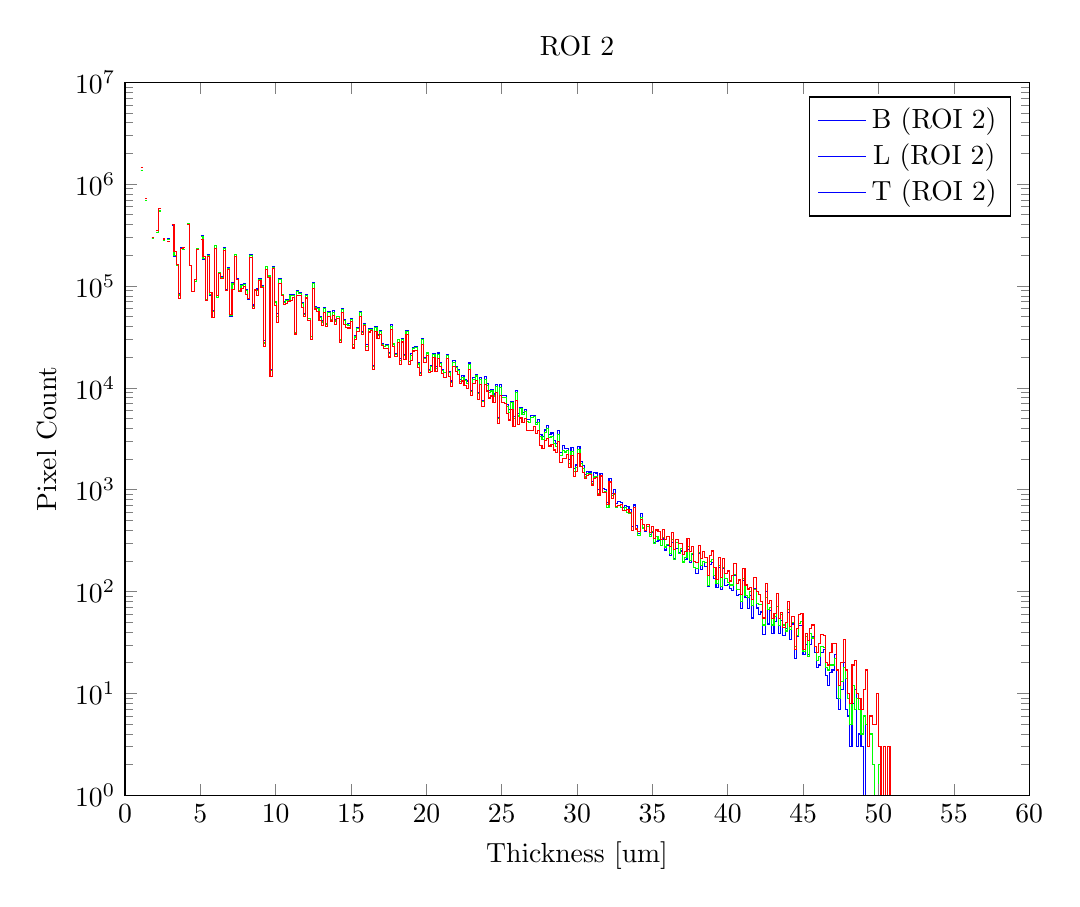
\begin{tikzpicture}

% Axis at [0.13 0.11 0.78 0.81]
\begin{semilogyaxis}[
axis on top,
scale only axis,
width=4.52083in,
height=3.56562in,
xmin=0, xmax=60,
ymin=1, ymax=1e+007,
xlabel={Thickness [um]},
ylabel={Pixel Count},
title={ROI 2},
legend entries={B (ROI 2),L (ROI 2),T (ROI 2)}
]

\addplot [
color=blue,
solid
]coordinates{
 (1.036,0) (1.036,1.35019e+006) (1.036,1.35019e+006) (1.184,1.35019e+006) (1.184,0)
};

\addplot [
color=blue,
solid
]coordinates{
 (1.332,0) (1.332,685760) (1.332,685760) (1.48,685760) (1.48,0)
};

\addplot [
color=blue,
solid
]coordinates{
 (1.776,0) (1.776,293972) (1.776,293972) (1.924,293972) (1.924,0)
};

\addplot [
color=blue,
solid
]coordinates{
 (2.072,0) (2.072,335526) (2.072,335526) (2.22,335526) (2.22,542864) (2.22,542864) (2.368,542864) (2.368,0)
};

\addplot [
color=blue,
solid
]coordinates{
 (2.516,0) (2.516,277964) (2.516,277964) (2.664,277964) (2.664,0)
};

\addplot [
color=blue,
solid
]coordinates{
 (2.812,0) (2.812,291708) (2.812,291708) (2.96,291708) (2.96,0)
};

\addplot [
color=blue,
solid
]coordinates{
 (3.108,0) (3.108,396821) (3.108,396821) (3.256,396821) (3.256,194759) (3.256,194759) (3.404,194759) (3.404,160501) (3.404,160501) (3.552,160501) (3.552,83446) (3.552,83446) (3.7,83446) (3.7,237451) (3.7,237451) (3.848,237451) (3.848,228756) (3.848,228756) (3.996,228756) (3.996,0)
};

\addplot [
color=blue,
solid
]coordinates{
 (4.144,0) (4.144,412179) (4.144,412179) (4.292,412179) (4.292,159008) (4.292,159008) (4.44,159008) (4.44,88316) (4.44,88316) (4.588,88316) (4.588,110875) (4.588,110875) (4.736,110875) (4.736,233086) (4.736,233086) (4.884,233086) (4.884,0)
};

\addplot [
color=blue,
solid
]coordinates{
 (5.032,0) (5.032,312684) (5.032,312684) (5.18,312684) (5.18,183652) (5.18,183652) (5.328,183652) (5.328,72181) (5.328,72181) (5.476,72181) (5.476,203079) (5.476,203079) (5.624,203079) (5.624,81348) (5.624,81348) (5.772,81348) (5.772,57975) (5.772,57975) (5.92,57975) (5.92,251609) (5.92,251609) (6.068,251609) (6.068,77366) (6.068,77366) (6.216,77366) (6.216,133350) (6.216,133350) (6.364,133350) (6.364,122621) (6.364,122621) (6.512,122621) (6.512,238856) (6.512,238856) (6.66,238856) (6.66,91357) (6.66,91357) (6.808,91357) (6.808,151741) (6.808,151741) (6.956,151741) (6.956,50498) (6.956,50498) (7.104,50498) (7.104,107490) (7.104,107490) (7.252,107490) (7.252,202530) (7.252,202530) (7.4,202530) (7.4,117031) (7.4,117031) (7.548,117031) (7.548,90436) (7.548,90436) (7.696,90436) (7.696,102532) (7.696,102532) (7.844,102532) (7.844,104440) (7.844,104440) (7.992,104440) (7.992,92683) (7.992,92683) (8.14,92683) (8.14,74215) (8.14,74215) (8.288,74215) (8.288,202114) (8.288,202114) (8.436,202114) (8.436,64957) (8.436,64957) (8.584,64957) (8.584,92371) (8.584,92371) (8.732,92371) (8.732,93414) (8.732,93414) (8.88,93414) (8.88,117976) (8.88,117976) (9.028,117976) (9.028,100101) (9.028,100101) (9.176,100101) (9.176,29238) (9.176,29238) (9.324,29238) (9.324,156517) (9.324,156517) (9.472,156517) (9.472,126816) (9.472,126816) (9.62,126816) (9.62,15051) (9.62,15051) (9.768,15051) (9.768,154257) (9.768,154257) (9.916,154257) (9.916,70476) (9.916,70476) (10.064,70476) (10.064,53144) (10.064,53144) (10.212,53144) (10.212,118524) (10.212,118524) (10.36,118524) (10.36,80872) (10.36,80872) (10.508,80872) (10.508,69883) (10.508,69883) (10.656,69883) (10.656,73248) (10.656,73248) (10.804,73248) (10.804,73056) (10.804,73056) (10.952,73056) (10.952,81943) (10.952,81943) (11.1,81943) (11.1,82336) (11.1,82336) (11.248,82336) (11.248,34870) (11.248,34870) (11.396,34870) (11.396,90165) (11.396,90165) (11.544,90165) (11.544,85591) (11.544,85591) (11.692,85591) (11.692,69000) (11.692,69000) (11.84,69000) (11.84,53426) (11.84,53426) (11.988,53426) (11.988,82174) (11.988,82174) (12.136,82174) (12.136,48163) (12.136,48163) (12.284,48163) (12.284,32134) (12.284,32134) (12.432,32134) (12.432,108019) (12.432,108019) (12.58,108019) (12.58,62385) (12.58,62385) (12.728,62385) (12.728,60667) (12.728,60667) (12.876,60667) (12.876,49739) (12.876,49739) (13.024,49739) (13.024,45786) (13.024,45786) (13.172,45786) (13.172,60793) (13.172,60793) (13.32,60793) (13.32,43213) (13.32,43213) (13.468,43213) (13.468,55618) (13.468,55618) (13.616,55618) (13.616,47136) (13.616,47136) (13.764,47136) (13.764,56912) (13.764,56912) (13.912,56912) (13.912,46283) (13.912,46283) (14.06,46283) (14.06,50548) (14.06,50548) (14.208,50548) (14.208,29965) (14.208,29965) (14.356,29965) (14.356,60117) (14.356,60117) (14.504,60117) (14.504,46819) (14.504,46819) (14.652,46819) (14.652,41596) (14.652,41596) (14.8,41596) (14.8,42480) (14.8,42480) (14.948,42480) (14.948,47563) (14.948,47563) (15.096,47563) (15.096,26856) (15.096,26856) (15.244,26856) (15.244,32540) (15.244,32540) (15.392,32540) (15.392,38902) (15.392,38902) (15.54,38902) (15.54,55705) (15.54,55705) (15.688,55705) (15.688,35274) (15.688,35274) (15.836,35274) (15.836,42541) (15.836,42541) (15.984,42541) (15.984,26751) (15.984,26751) (16.132,26751) (16.132,38544) (16.132,38544) (16.28,38544) (16.28,38598) (16.28,38598) (16.428,38598) (16.428,16569) (16.428,16569) (16.576,16569) (16.576,40183) (16.576,40183) (16.724,40183) (16.724,33424) (16.724,33424) (16.872,33424) (16.872,36182) (16.872,36182) (17.02,36182) (17.02,27454) (17.02,27454) (17.168,27454) (17.168,25694) (17.168,25694) (17.316,25694) (17.316,26744) (17.316,26744) (17.464,26744) (17.464,22294) (17.464,22294) (17.612,22294) (17.612,41553) (17.612,41553) (17.76,41553) (17.76,27281) (17.76,27281) (17.908,27281) (17.908,21482) (17.908,21482) (18.056,21482) (18.056,30080) (18.056,30080) (18.204,30080) (18.204,19250) (18.204,19250) (18.352,19250) (18.352,30286) (18.352,30286) (18.5,30286) (18.5,21288) (18.5,21288) (18.648,21288) (18.648,36326) (18.648,36326) (18.796,36326) (18.796,18274) (18.796,18274) (18.944,18274) (18.944,21641) (18.944,21641) (19.092,21641) (19.092,24727) (19.092,24727) (19.24,24727) (19.24,25295) (19.24,25295) (19.388,25295) (19.388,17520) (19.388,17520) (19.536,17520) (19.536,14187) (19.536,14187) (19.684,14187) (19.684,30537) (19.684,30537) (19.832,30537) (19.832,19960) (19.832,19960) (19.98,19960) (19.98,22371) (19.98,22371) (20.128,22371) (20.128,15021) (20.128,15021) (20.276,15021) (20.276,16606) (20.276,16606) (20.424,16606) (20.424,21909) (20.424,21909) (20.572,21909) (20.572,16093) (20.572,16093) (20.72,16093) (20.72,21989) (20.72,21989) (20.868,21989) (20.868,17685) (20.868,17685) (21.016,17685) (21.016,15267) (21.016,15267) (21.164,15267) (21.164,14141) (21.164,14141) (21.312,14141) (21.312,21333) (21.312,21333) (21.46,21333) (21.46,14301) (21.46,14301) (21.608,14301) (21.608,11654) (21.608,11654) (21.756,11654) (21.756,18504) (21.756,18504) (21.904,18504) (21.904,16269) (21.904,16269) (22.052,16269) (22.052,15120) (22.052,15120) (22.2,15120) (22.2,12028) (22.2,12028) (22.348,12028) (22.348,13099) (22.348,13099) (22.496,13099) (22.496,11937) (22.496,11937) (22.644,11937) (22.644,11650) (22.644,11650) (22.792,11650) (22.792,17521) (22.792,17521) (22.94,17521) (22.94,9461) (22.94,9461) (23.088,9461) (23.088,12635) (23.088,12635) (23.236,12635) (23.236,13566) (23.236,13566) (23.384,13566) (23.384,8942) (23.384,8942) (23.532,8942) (23.532,12681) (23.532,12681) (23.68,12681) (23.68,7517) (23.68,7517) (23.828,7517) (23.828,12824) (23.828,12824) (23.976,12824) (23.976,10928) (23.976,10928) (24.124,10928) (24.124,9493) (24.124,9493) (24.272,9493) (24.272,9593) (24.272,9593) (24.42,9593) (24.42,8688) (24.42,8688) (24.568,8688) (24.568,10838) (24.568,10838) (24.716,10838) (24.716,5148) (24.716,5148) (24.864,5148) (24.864,10691) (24.864,10691) (25.012,10691) (25.012,8478) (25.012,8478) (25.16,8478) (25.16,8447) (25.16,8447) (25.308,8447) (25.308,6831) (25.308,6831) (25.456,6831) (25.456,6134) (25.456,6134) (25.604,6134) (25.604,7402) (25.604,7402) (25.752,7402) (25.752,5276) (25.752,5276) (25.9,5276) (25.9,9481) (25.9,9481) (26.048,9481) (26.048,5542) (26.048,5542) (26.196,5542) (26.196,6368) (26.196,6368) (26.344,6368) (26.344,5769) (26.344,5769) (26.492,5769) (26.492,6167) (26.492,6167) (26.64,6167) (26.64,4885) (26.64,4885) (26.788,4885) (26.788,4860) (26.788,4860) (26.936,4860) (26.936,5387) (26.936,5387) (27.084,5387) (27.084,5383) (27.084,5383) (27.232,5383) (27.232,4555) (27.232,4555) (27.38,4555) (27.38,4874) (27.38,4874) (27.528,4874) (27.528,3464) (27.528,3464) (27.676,3464) (27.676,3296) (27.676,3296) (27.824,3296) (27.824,3855) (27.824,3855) (27.972,3855) (27.972,4235) (27.972,4235) (28.12,4235) (28.12,3457) (28.12,3457) (28.268,3457) (28.268,3605) (28.268,3605) (28.416,3605) (28.416,3059) (28.416,3059) (28.564,3059) (28.564,2844) (28.564,2844) (28.712,2844) (28.712,3778) (28.712,3778) (28.86,3778) (28.86,2331) (28.86,2331) (29.008,2331) (29.008,2724) (29.008,2724) (29.156,2724) (29.156,2562) (29.156,2562) (29.304,2562) (29.304,2554) (29.304,2554) (29.452,2554) (29.452,1978) (29.452,1978) (29.6,1978) (29.6,2569) (29.6,2569) (29.748,2569) (29.748,1608) (29.748,1608) (29.896,1608) (29.896,1749) (29.896,1749) (30.044,1749) (30.044,2642) (30.044,2642) (30.192,2642) (30.192,1903) (30.192,1903) (30.34,1903) (30.34,1731) (30.34,1731) (30.488,1731) (30.488,1422) (30.488,1422) (30.636,1422) (30.636,1508) (30.636,1508) (30.784,1508) (30.784,1491) (30.784,1491) (30.932,1491) (30.932,1201) (30.932,1201) (31.08,1201) (31.08,1460) (31.08,1460) (31.228,1460) (31.228,1457) (31.228,1457) (31.376,1457) (31.376,1001) (31.376,1001) (31.524,1001) (31.524,1449) (31.524,1449) (31.672,1449) (31.672,1017) (31.672,1017) (31.82,1017) (31.82,1014) (31.82,1014) (31.968,1014) (31.968,754) (31.968,754) (32.116,754) (32.116,1296) (32.116,1296) (32.264,1296) (32.264,919) (32.264,919) (32.412,919) (32.412,999) (32.412,999) (32.56,999) (32.56,738) (32.56,738) (32.708,738) (32.708,763) (32.708,763) (32.856,763) (32.856,755) (32.856,755) (33.004,755) (33.004,674) (33.004,674) (33.152,674) (33.152,699) (33.152,699) (33.3,699) (33.3,683) (33.3,683) (33.448,683) (33.448,641) (33.448,641) (33.596,641) (33.596,431) (33.596,431) (33.744,431) (33.744,707) (33.744,707) (33.892,707) (33.892,447) (33.892,447) (34.04,447) (34.04,374) (34.04,374) (34.188,374) (34.188,588) (34.188,588) (34.336,588) (34.336,424) (34.336,424) (34.484,424) (34.484,389) (34.484,389) (34.632,389) (34.632,439) (34.632,439) (34.78,439) (34.78,360) (34.78,360) (34.928,360) (34.928,382) (34.928,382) (35.076,382) (35.076,300) (35.076,300) (35.224,300) (35.224,309) (35.224,309) (35.372,309) (35.372,314) (35.372,314) (35.52,314) (35.52,281) (35.52,281) (35.668,281) (35.668,328) (35.668,328) (35.816,328) (35.816,256) (35.816,256) (35.964,256) (35.964,284) (35.964,284) (36.112,284) (36.112,227) (36.112,227) (36.26,227) (36.26,303) (36.26,303) (36.408,303) (36.408,211) (36.408,211) (36.556,211) (36.556,264) (36.556,264) (36.704,264) (36.704,244) (36.704,244) (36.852,244) (36.852,250) (36.852,250) (37,250) (37,191) (37,191) (37.148,191) (37.148,205) (37.148,205) (37.296,205) (37.296,258) (37.296,258) (37.444,258) (37.444,193) (37.444,193) (37.592,193) (37.592,229) (37.592,229) (37.74,229) (37.74,171) (37.74,171) (37.888,171) (37.888,150) (37.888,150) (38.036,150) (38.036,239) (38.036,239) (38.184,239) (38.184,163) (38.184,163) (38.332,163) (38.332,196) (38.332,196) (38.48,196) (38.48,175) (38.48,175) (38.628,175) (38.628,111) (38.628,111) (38.776,111) (38.776,186) (38.776,186) (38.924,186) (38.924,192) (38.924,192) (39.072,192) (39.072,134) (39.072,134) (39.22,134) (39.22,109) (39.22,109) (39.368,109) (39.368,172) (39.368,172) (39.516,172) (39.516,104) (39.516,104) (39.664,104) (39.664,167) (39.664,167) (39.812,167) (39.812,115) (39.812,115) (39.96,115) (39.96,117) (39.96,117) (40.108,117) (40.108,108) (40.108,108) (40.256,108) (40.256,103) (40.256,103) (40.404,103) (40.404,145) (40.404,145) (40.552,145) (40.552,92) (40.552,92) (40.7,92) (40.7,93) (40.7,93) (40.848,93) (40.848,68) (40.848,68) (40.996,68) (40.996,129) (40.996,129) (41.144,129) (41.144,87) (41.144,87) (41.292,87) (41.292,68) (41.292,68) (41.44,68) (41.44,91) (41.44,91) (41.588,91) (41.588,55) (41.588,55) (41.736,55) (41.736,108) (41.736,108) (41.884,108) (41.884,69) (41.884,69) (42.032,69) (42.032,59) (42.032,59) (42.18,59) (42.18,63) (42.18,63) (42.328,63) (42.328,38) (42.328,38) (42.476,38) (42.476,100) (42.476,100) (42.624,100) (42.624,48) (42.624,48) (42.772,48) (42.772,65) (42.772,65) (42.92,65) (42.92,39) (42.92,39) (43.068,39) (43.068,51) (43.068,51) (43.216,51) (43.216,72) (43.216,72) (43.364,72) (43.364,39) (43.364,39) (43.512,39) (43.512,52) (43.512,52) (43.66,52) (43.66,37) (43.66,37) (43.808,37) (43.808,43) (43.808,43) (43.956,43) (43.956,62) (43.956,62) (44.104,62) (44.104,34) (44.104,34) (44.252,34) (44.252,48) (44.252,48) (44.4,48) (44.4,22) (44.4,22) (44.548,22) (44.548,36) (44.548,36) (44.696,36) (44.696,46) (44.696,46) (44.844,46) (44.844,46) (44.844,46) (44.992,46) (44.992,24) (44.992,24) (45.14,24) (45.14,30) (45.14,30) (45.288,30) (45.288,24) (45.288,24) (45.436,24) (45.436,30) (45.436,30) (45.584,30) (45.584,36) (45.584,36) (45.732,36) (45.732,25) (45.732,25) (45.88,25) (45.88,18) (45.88,18) (46.028,18) (46.028,19) (46.028,19) (46.176,19) (46.176,25) (46.176,25) (46.324,25) (46.324,27) (46.324,27) (46.472,27) (46.472,15) (46.472,15) (46.62,15) (46.62,12) (46.62,12) (46.768,12) (46.768,16) (46.768,16) (46.916,16) (46.916,17) (46.916,17) (47.064,17) (47.064,24) (47.064,24) (47.212,24) (47.212,9) (47.212,9) (47.36,9) (47.36,7) (47.36,7) (47.508,7) (47.508,11) (47.508,11) (47.656,11) (47.656,20) (47.656,20) (47.804,20) (47.804,7) (47.804,7) (47.952,7) (47.952,6) (47.952,6) (48.1,6) (48.1,3) (48.1,3) (48.248,3) (48.248,8) (48.248,8) (48.396,8) (48.396,11) (48.396,11) (48.544,11) (48.544,3) (48.544,3) (48.692,3) (48.692,4) (48.692,4) (48.84,4) (48.84,3) (48.84,3) (48.988,3) (48.988,1)
};

\addplot [
color=blue,
solid
]coordinates{
 (49.136,1) (49.136,5) (49.136,5) (49.284,5) (49.284,0)
};

\addplot [
color=green,
solid
]coordinates{
 (1.036,0) (1.036,1.36333e+006) (1.036,1.36333e+006) (1.184,1.36333e+006) (1.184,0)
};

\addplot [
color=green,
solid
]coordinates{
 (1.332,0) (1.332,687983) (1.332,687983) (1.48,687983) (1.48,0)
};

\addplot [
color=green,
solid
]coordinates{
 (1.776,0) (1.776,293732) (1.776,293732) (1.924,293732) (1.924,0)
};

\addplot [
color=green,
solid
]coordinates{
 (2.072,0) (2.072,337158) (2.072,337158) (2.22,337158) (2.22,544498) (2.22,544498) (2.368,544498) (2.368,0)
};

\addplot [
color=green,
solid
]coordinates{
 (2.516,0) (2.516,279247) (2.516,279247) (2.664,279247) (2.664,0)
};

\addplot [
color=green,
solid
]coordinates{
 (2.812,0) (2.812,285011) (2.812,285011) (2.96,285011) (2.96,0)
};

\addplot [
color=green,
solid
]coordinates{
 (3.108,0) (3.108,397861) (3.108,397861) (3.256,397861) (3.256,199346) (3.256,199346) (3.404,199346) (3.404,160589) (3.404,160589) (3.552,160589) (3.552,81554) (3.552,81554) (3.7,81554) (3.7,233978) (3.7,233978) (3.848,233978) (3.848,229951) (3.848,229951) (3.996,229951) (3.996,0)
};

\addplot [
color=green,
solid
]coordinates{
 (4.144,0) (4.144,410027) (4.144,410027) (4.292,410027) (4.292,159578) (4.292,159578) (4.44,159578) (4.44,87812) (4.44,87812) (4.588,87812) (4.588,110705) (4.588,110705) (4.736,110705) (4.736,231591) (4.736,231591) (4.884,231591) (4.884,0)
};

\addplot [
color=green,
solid
]coordinates{
 (5.032,0) (5.032,306877) (5.032,306877) (5.18,306877) (5.18,186332) (5.18,186332) (5.328,186332) (5.328,72729) (5.328,72729) (5.476,72729) (5.476,200153) (5.476,200153) (5.624,200153) (5.624,82649) (5.624,82649) (5.772,82649) (5.772,55923) (5.772,55923) (5.92,55923) (5.92,247346) (5.92,247346) (6.068,247346) (6.068,77268) (6.068,77268) (6.216,77268) (6.216,135430) (6.216,135430) (6.364,135430) (6.364,121775) (6.364,121775) (6.512,121775) (6.512,235153) (6.512,235153) (6.66,235153) (6.66,90911) (6.66,90911) (6.808,90911) (6.808,149549) (6.808,149549) (6.956,149549) (6.956,50810) (6.956,50810) (7.104,50810) (7.104,104509) (7.104,104509) (7.252,104509) (7.252,202899) (7.252,202899) (7.4,202899) (7.4,115960) (7.4,115960) (7.548,115960) (7.548,89976) (7.548,89976) (7.696,89976) (7.696,101056) (7.696,101056) (7.844,101056) (7.844,102429) (7.844,102429) (7.992,102429) (7.992,89934) (7.992,89934) (8.14,89934) (8.14,74882) (8.14,74882) (8.288,74882) (8.288,200590) (8.288,200590) (8.436,200590) (8.436,63428) (8.436,63428) (8.584,63428) (8.584,92216) (8.584,92216) (8.732,92216) (8.732,90374) (8.732,90374) (8.88,90374) (8.88,116600) (8.88,116600) (9.028,116600) (9.028,99546) (9.028,99546) (9.176,99546) (9.176,27520) (9.176,27520) (9.324,27520) (9.324,155577) (9.324,155577) (9.472,155577) (9.472,125212) (9.472,125212) (9.62,125212) (9.62,14761) (9.62,14761) (9.768,14761) (9.768,151976) (9.768,151976) (9.916,151976) (9.916,69531) (9.916,69531) (10.064,69531) (10.064,50527) (10.064,50527) (10.212,50527) (10.212,116384) (10.212,116384) (10.36,116384) (10.36,81560) (10.36,81560) (10.508,81560) (10.508,68601) (10.508,68601) (10.656,68601) (10.656,72114) (10.656,72114) (10.804,72114) (10.804,71899) (10.804,71899) (10.952,71899) (10.952,79858) (10.952,79858) (11.1,79858) (11.1,80683) (11.1,80683) (11.248,80683) (11.248,34907) (11.248,34907) (11.396,34907) (11.396,88788) (11.396,88788) (11.544,88788) (11.544,84036) (11.544,84036) (11.692,84036) (11.692,67309) (11.692,67309) (11.84,67309) (11.84,52419) (11.84,52419) (11.988,52419) (11.988,80537) (11.988,80537) (12.136,80537) (12.136,47692) (12.136,47692) (12.284,47692) (12.284,31621) (12.284,31621) (12.432,31621) (12.432,105376) (12.432,105376) (12.58,105376) (12.58,61549) (12.58,61549) (12.728,61549) (12.728,59629) (12.728,59629) (12.876,59629) (12.876,48871) (12.876,48871) (13.024,48871) (13.024,44244) (13.024,44244) (13.172,44244) (13.172,59702) (13.172,59702) (13.32,59702) (13.32,42276) (13.32,42276) (13.468,42276) (13.468,54692) (13.468,54692) (13.616,54692) (13.616,46576) (13.616,46576) (13.764,46576) (13.764,55168) (13.764,55168) (13.912,55168) (13.912,45280) (13.912,45280) (14.06,45280) (14.06,49785) (14.06,49785) (14.208,49785) (14.208,29436) (14.208,29436) (14.356,29436) (14.356,58609) (14.356,58609) (14.504,58609) (14.504,45700) (14.504,45700) (14.652,45700) (14.652,41446) (14.652,41446) (14.8,41446) (14.8,40849) (14.8,40849) (14.948,40849) (14.948,46909) (14.948,46909) (15.096,46909) (15.096,26434) (15.096,26434) (15.244,26434) (15.244,31524) (15.244,31524) (15.392,31524) (15.392,38003) (15.392,38003) (15.54,38003) (15.54,54325) (15.54,54325) (15.688,54325) (15.688,34654) (15.688,34654) (15.836,34654) (15.836,42211) (15.836,42211) (15.984,42211) (15.984,25650) (15.984,25650) (16.132,25650) (16.132,37607) (16.132,37607) (16.28,37607) (16.28,37726) (16.28,37726) (16.428,37726) (16.428,16151) (16.428,16151) (16.576,16151) (16.576,39270) (16.576,39270) (16.724,39270) (16.724,32589) (16.724,32589) (16.872,32589) (16.872,35538) (16.872,35538) (17.02,35538) (17.02,26774) (17.02,26774) (17.168,26774) (17.168,25424) (17.168,25424) (17.316,25424) (17.316,26003) (17.316,26003) (17.464,26003) (17.464,21779) (17.464,21779) (17.612,21779) (17.612,40321) (17.612,40321) (17.76,40321) (17.76,26946) (17.76,26946) (17.908,26946) (17.908,21172) (17.908,21172) (18.056,21172) (18.056,29568) (18.056,29568) (18.204,29568) (18.204,18635) (18.204,18635) (18.352,18635) (18.352,29685) (18.352,29685) (18.5,29685) (18.5,20733) (18.5,20733) (18.648,20733) (18.648,35629) (18.648,35629) (18.796,35629) (18.796,18016) (18.796,18016) (18.944,18016) (18.944,20729) (18.944,20729) (19.092,20729) (19.092,24357) (19.092,24357) (19.24,24357) (19.24,24835) (19.24,24835) (19.388,24835) (19.388,17137) (19.388,17137) (19.536,17137) (19.536,13779) (19.536,13779) (19.684,13779) (19.684,29537) (19.684,29537) (19.832,29537) (19.832,19376) (19.832,19376) (19.98,19376) (19.98,21972) (19.98,21972) (20.128,21972) (20.128,14712) (20.128,14712) (20.276,14712) (20.276,16189) (20.276,16189) (20.424,16189) (20.424,21286) (20.424,21286) (20.572,21286) (20.572,15513) (20.572,15513) (20.72,15513) (20.72,21325) (20.72,21325) (20.868,21325) (20.868,17261) (20.868,17261) (21.016,17261) (21.016,14687) (21.016,14687) (21.164,14687) (21.164,14003) (21.164,14003) (21.312,14003) (21.312,20587) (21.312,20587) (21.46,20587) (21.46,14012) (21.46,14012) (21.608,14012) (21.608,11303) (21.608,11303) (21.756,11303) (21.756,17720) (21.756,17720) (21.904,17720) (21.904,15753) (21.904,15753) (22.052,15753) (22.052,14745) (22.052,14745) (22.2,14745) (22.2,11626) (22.2,11626) (22.348,11626) (22.348,12693) (22.348,12693) (22.496,12693) (22.496,11693) (22.496,11693) (22.644,11693) (22.644,10983) (22.644,10983) (22.792,10983) (22.792,16876) (22.792,16876) (22.94,16876) (22.94,9224) (22.94,9224) (23.088,9224) (23.088,12155) (23.088,12155) (23.236,12155) (23.236,13054) (23.236,13054) (23.384,13054) (23.384,8716) (23.384,8716) (23.532,8716) (23.532,12019) (23.532,12019) (23.68,12019) (23.68,7300) (23.68,7300) (23.828,7300) (23.828,12120) (23.828,12120) (23.976,12120) (23.976,10590) (23.976,10590) (24.124,10590) (24.124,9079) (24.124,9079) (24.272,9079) (24.272,9296) (24.272,9296) (24.42,9296) (24.42,8316) (24.42,8316) (24.568,8316) (24.568,10320) (24.568,10320) (24.716,10320) (24.716,5008) (24.716,5008) (24.864,5008) (24.864,10092) (24.864,10092) (25.012,10092) (25.012,8068) (25.012,8068) (25.16,8068) (25.16,8064) (25.16,8064) (25.308,8064) (25.308,6619) (25.308,6619) (25.456,6619) (25.456,5728) (25.456,5728) (25.604,5728) (25.604,7221) (25.604,7221) (25.752,7221) (25.752,5009) (25.752,5009) (25.9,5009) (25.9,8991) (25.9,8991) (26.048,8991) (26.048,5284) (26.048,5284) (26.196,5284) (26.196,6225) (26.196,6225) (26.344,6225) (26.344,5468) (26.344,5468) (26.492,5468) (26.492,5912) (26.492,5912) (26.64,5912) (26.64,4676) (26.64,4676) (26.788,4676) (26.788,4568) (26.788,4568) (26.936,4568) (26.936,5089) (26.936,5089) (27.084,5089) (27.084,5196) (27.084,5196) (27.232,5196) (27.232,4374) (27.232,4374) (27.38,4374) (27.38,4574) (27.38,4574) (27.528,4574) (27.528,3332) (27.528,3332) (27.676,3332) (27.676,3084) (27.676,3084) (27.824,3084) (27.824,3675) (27.824,3675) (27.972,3675) (27.972,3948) (27.972,3948) (28.12,3948) (28.12,3264) (28.12,3264) (28.268,3264) (28.268,3335) (28.268,3335) (28.416,3335) (28.416,2827) (28.416,2827) (28.564,2827) (28.564,2675) (28.564,2675) (28.712,2675) (28.712,3482) (28.712,3482) (28.86,3482) (28.86,2146) (28.86,2146) (29.008,2146) (29.008,2446) (29.008,2446) (29.156,2446) (29.156,2341) (29.156,2341) (29.304,2341) (29.304,2432) (29.304,2432) (29.452,2432) (29.452,1821) (29.452,1821) (29.6,1821) (29.6,2384) (29.6,2384) (29.748,2384) (29.748,1499) (29.748,1499) (29.896,1499) (29.896,1639) (29.896,1639) (30.044,1639) (30.044,2465) (30.044,2465) (30.192,2465) (30.192,1794) (30.192,1794) (30.34,1794) (30.34,1599) (30.34,1599) (30.488,1599) (30.488,1333) (30.488,1333) (30.636,1333) (30.636,1430) (30.636,1430) (30.784,1430) (30.784,1431) (30.784,1431) (30.932,1431) (30.932,1142) (30.932,1142) (31.08,1142) (31.08,1331) (31.08,1331) (31.228,1331) (31.228,1340) (31.228,1340) (31.376,1340) (31.376,918) (31.376,918) (31.524,918) (31.524,1362) (31.524,1362) (31.672,1362) (31.672,945) (31.672,945) (31.82,945) (31.82,952) (31.82,952) (31.968,952) (31.968,669) (31.968,669) (32.116,669) (32.116,1167) (32.116,1167) (32.264,1167) (32.264,877) (32.264,877) (32.412,877) (32.412,904) (32.412,904) (32.56,904) (32.56,667) (32.56,667) (32.708,667) (32.708,704) (32.708,704) (32.856,704) (32.856,668) (32.856,668) (33.004,668) (33.004,619) (33.004,619) (33.152,619) (33.152,666) (33.152,666) (33.3,666) (33.3,603) (33.3,603) (33.448,603) (33.448,584) (33.448,584) (33.596,584) (33.596,394) (33.596,394) (33.744,394) (33.744,670) (33.744,670) (33.892,670) (33.892,408) (33.892,408) (34.04,408) (34.04,352) (34.04,352) (34.188,352) (34.188,535) (34.188,535) (34.336,535) (34.336,421) (34.336,421) (34.484,421) (34.484,399) (34.484,399) (34.632,399) (34.632,437) (34.632,437) (34.78,437) (34.78,345) (34.78,345) (34.928,345) (34.928,390) (34.928,390) (35.076,390) (35.076,299) (35.076,299) (35.224,299) (35.224,347) (35.224,347) (35.372,347) (35.372,325) (35.372,325) (35.52,325) (35.52,284) (35.52,284) (35.668,284) (35.668,341) (35.668,341) (35.816,341) (35.816,274) (35.816,274) (35.964,274) (35.964,288) (35.964,288) (36.112,288) (36.112,238) (36.112,238) (36.26,238) (36.26,327) (36.26,327) (36.408,327) (36.408,206) (36.408,206) (36.556,206) (36.556,303) (36.556,303) (36.704,303) (36.704,238) (36.704,238) (36.852,238) (36.852,264) (36.852,264) (37,264) (37,195) (37,195) (37.148,195) (37.148,214) (37.148,214) (37.296,214) (37.296,277) (37.296,277) (37.444,277) (37.444,200) (37.444,200) (37.592,200) (37.592,237) (37.592,237) (37.74,237) (37.74,172) (37.74,172) (37.888,172) (37.888,168) (37.888,168) (38.036,168) (38.036,242) (38.036,242) (38.184,242) (38.184,180) (38.184,180) (38.332,180) (38.332,197) (38.332,197) (38.48,197) (38.48,193) (38.48,193) (38.628,193) (38.628,114) (38.628,114) (38.776,114) (38.776,196) (38.776,196) (38.924,196) (38.924,207) (38.924,207) (39.072,207) (39.072,143) (39.072,143) (39.22,143) (39.22,120) (39.22,120) (39.368,120) (39.368,181) (39.368,181) (39.516,181) (39.516,112) (39.516,112) (39.664,112) (39.664,174) (39.664,174) (39.812,174) (39.812,133) (39.812,133) (39.96,133) (39.96,123) (39.96,123) (40.108,123) (40.108,116) (40.108,116) (40.256,116) (40.256,116) (40.256,116) (40.404,116) (40.404,148) (40.404,148) (40.552,148) (40.552,105) (40.552,105) (40.7,105) (40.7,105) (40.7,105) (40.848,105) (40.848,80) (40.848,80) (40.996,80) (40.996,135) (40.996,135) (41.144,135) (41.144,91) (41.144,91) (41.292,91) (41.292,87) (41.292,87) (41.44,87) (41.44,101) (41.44,101) (41.588,101) (41.588,73) (41.588,73) (41.736,73) (41.736,104) (41.736,104) (41.884,104) (41.884,76) (41.884,76) (42.032,76) (42.032,74) (42.032,74) (42.18,74) (42.18,74) (42.18,74) (42.328,74) (42.328,47) (42.328,47) (42.476,47) (42.476,87) (42.476,87) (42.624,87) (42.624,67) (42.624,67) (42.772,67) (42.772,70) (42.772,70) (42.92,70) (42.92,47) (42.92,47) (43.068,47) (43.068,57) (43.068,57) (43.216,57) (43.216,71) (43.216,71) (43.364,71) (43.364,46) (43.364,46) (43.512,46) (43.512,59) (43.512,59) (43.66,59) (43.66,47) (43.66,47) (43.808,47) (43.808,41) (43.808,41) (43.956,41) (43.956,67) (43.956,67) (44.104,67) (44.104,42) (44.104,42) (44.252,42) (44.252,50) (44.252,50) (44.4,50) (44.4,29) (44.4,29) (44.548,29) (44.548,37) (44.548,37) (44.696,37) (44.696,49) (44.696,49) (44.844,49) (44.844,51) (44.844,51) (44.992,51) (44.992,26) (44.992,26) (45.14,26) (45.14,36) (45.14,36) (45.288,36) (45.288,23) (45.288,23) (45.436,23) (45.436,39) (45.436,39) (45.584,39) (45.584,35) (45.584,35) (45.732,35) (45.732,29) (45.732,29) (45.88,29) (45.88,21) (45.88,21) (46.028,21) (46.028,23) (46.028,23) (46.176,23) (46.176,29) (46.176,29) (46.324,29) (46.324,28) (46.324,28) (46.472,28) (46.472,18) (46.472,18) (46.62,18) (46.62,17) (46.62,17) (46.768,17) (46.768,19) (46.768,19) (46.916,19) (46.916,19) (46.916,19) (47.064,19) (47.064,22) (47.064,22) (47.212,22) (47.212,17) (47.212,17) (47.36,17) (47.36,9) (47.36,9) (47.508,9) (47.508,13) (47.508,13) (47.656,13) (47.656,18) (47.656,18) (47.804,18) (47.804,14) (47.804,14) (47.952,14) (47.952,9) (47.952,9) (48.1,9) (48.1,5) (48.1,5) (48.248,5) (48.248,12) (48.248,12) (48.396,12) (48.396,7) (48.396,7) (48.544,7) (48.544,9) (48.544,9) (48.692,9) (48.692,7) (48.692,7) (48.84,7) (48.84,4) (48.84,4) (48.988,4) (48.988,6) (48.988,6) (49.136,6) (49.136,5) (49.136,5) (49.284,5) (49.284,3) (49.284,3) (49.432,3) (49.432,4) (49.432,4) (49.58,4) (49.58,2) (49.58,2) (49.728,2) (49.728,1)
};

\addplot [
color=green,
solid
]coordinates{
 (50.024,1) (50.024,2) (50.024,2) (50.172,2) (50.172,0)
};

\addplot [
color=red,
solid
]coordinates{
 (1.036,0) (1.036,1.4485e+006) (1.036,1.4485e+006) (1.184,1.4485e+006) (1.184,0)
};

\addplot [
color=red,
solid
]coordinates{
 (1.332,0) (1.332,727487) (1.332,727487) (1.48,727487) (1.48,0)
};

\addplot [
color=red,
solid
]coordinates{
 (1.776,0) (1.776,298057) (1.776,298057) (1.924,298057) (1.924,0)
};

\addplot [
color=red,
solid
]coordinates{
 (2.072,0) (2.072,349564) (2.072,349564) (2.22,349564) (2.22,571545) (2.22,571545) (2.368,571545) (2.368,0)
};

\addplot [
color=red,
solid
]coordinates{
 (2.516,0) (2.516,288834) (2.516,288834) (2.664,288834) (2.664,0)
};

\addplot [
color=red,
solid
]coordinates{
 (2.812,0) (2.812,273934) (2.812,273934) (2.96,273934) (2.96,0)
};

\addplot [
color=red,
solid
]coordinates{
 (3.108,0) (3.108,399678) (3.108,399678) (3.256,399678) (3.256,217956) (3.256,217956) (3.404,217956) (3.404,161739) (3.404,161739) (3.552,161739) (3.552,75277) (3.552,75277) (3.7,75277) (3.7,231767) (3.7,231767) (3.848,231767) (3.848,237070) (3.848,237070) (3.996,237070) (3.996,0)
};

\addplot [
color=red,
solid
]coordinates{
 (4.144,0) (4.144,398237) (4.144,398237) (4.292,398237) (4.292,159809) (4.292,159809) (4.44,159809) (4.44,88342) (4.44,88342) (4.588,88342) (4.588,114780) (4.588,114780) (4.736,114780) (4.736,229342) (4.736,229342) (4.884,229342) (4.884,0)
};

\addplot [
color=red,
solid
]coordinates{
 (5.032,0) (5.032,285131) (5.032,285131) (5.18,285131) (5.18,194800) (5.18,194800) (5.328,194800) (5.328,72119) (5.328,72119) (5.476,72119) (5.476,194996) (5.476,194996) (5.624,194996) (5.624,87049) (5.624,87049) (5.772,87049) (5.772,49115) (5.772,49115) (5.92,49115) (5.92,235154) (5.92,235154) (6.068,235154) (6.068,79761) (6.068,79761) (6.216,79761) (6.216,131809) (6.216,131809) (6.364,131809) (6.364,118571) (6.364,118571) (6.512,118571) (6.512,224443) (6.512,224443) (6.66,224443) (6.66,90297) (6.66,90297) (6.808,90297) (6.808,144381) (6.808,144381) (6.956,144381) (6.956,52937) (6.956,52937) (7.104,52937) (7.104,92686) (7.104,92686) (7.252,92686) (7.252,193870) (7.252,193870) (7.4,193870) (7.4,116363) (7.4,116363) (7.548,116363) (7.548,87883) (7.548,87883) (7.696,87883) (7.696,94827) (7.696,94827) (7.844,94827) (7.844,98715) (7.844,98715) (7.992,98715) (7.992,81631) (7.992,81631) (8.14,81631) (8.14,75132) (8.14,75132) (8.288,75132) (8.288,189215) (8.288,189215) (8.436,189215) (8.436,60645) (8.436,60645) (8.584,60645) (8.584,91178) (8.584,91178) (8.732,91178) (8.732,81288) (8.732,81288) (8.88,81288) (8.88,113102) (8.88,113102) (9.028,113102) (9.028,95931) (9.028,95931) (9.176,95931) (9.176,25217) (9.176,25217) (9.324,25217) (9.324,144755) (9.324,144755) (9.472,144755) (9.472,119814) (9.472,119814) (9.62,119814) (9.62,12988) (9.62,12988) (9.768,12988) (9.768,147960) (9.768,147960) (9.916,147960) (9.916,64841) (9.916,64841) (10.064,64841) (10.064,44177) (10.064,44177) (10.212,44177) (10.212,106688) (10.212,106688) (10.36,106688) (10.36,80323) (10.36,80323) (10.508,80323) (10.508,65279) (10.508,65279) (10.656,65279) (10.656,67123) (10.656,67123) (10.804,67123) (10.804,70082) (10.804,70082) (10.952,70082) (10.952,71918) (10.952,71918) (11.1,71918) (11.1,77536) (11.1,77536) (11.248,77536) (11.248,33780) (11.248,33780) (11.396,33780) (11.396,80727) (11.396,80727) (11.544,80727) (11.544,80397) (11.544,80397) (11.692,80397) (11.692,61598) (11.692,61598) (11.84,61598) (11.84,50010) (11.84,50010) (11.988,50010) (11.988,76079) (11.988,76079) (12.136,76079) (12.136,45457) (12.136,45457) (12.284,45457) (12.284,29935) (12.284,29935) (12.432,29935) (12.432,95253) (12.432,95253) (12.58,95253) (12.58,59372) (12.58,59372) (12.728,59372) (12.728,56652) (12.728,56652) (12.876,56652) (12.876,46101) (12.876,46101) (13.024,46101) (13.024,40536) (13.024,40536) (13.172,40536) (13.172,55090) (13.172,55090) (13.32,55090) (13.32,39760) (13.32,39760) (13.468,39760) (13.468,50313) (13.468,50313) (13.616,50313) (13.616,45262) (13.616,45262) (13.764,45262) (13.764,50780) (13.764,50780) (13.912,50780) (13.912,41810) (13.912,41810) (14.06,41810) (14.06,47488) (14.06,47488) (14.208,47488) (14.208,28039) (14.208,28039) (14.356,28039) (14.356,54492) (14.356,54492) (14.504,54492) (14.504,41576) (14.504,41576) (14.652,41576) (14.652,38900) (14.652,38900) (14.8,38900) (14.8,38648) (14.8,38648) (14.948,38648) (14.948,44769) (14.948,44769) (15.096,44769) (15.096,24587) (15.096,24587) (15.244,24587) (15.244,29665) (15.244,29665) (15.392,29665) (15.392,35369) (15.392,35369) (15.54,35369) (15.54,49755) (15.54,49755) (15.688,49755) (15.688,33236) (15.688,33236) (15.836,33236) (15.836,40596) (15.836,40596) (15.984,40596) (15.984,23119) (15.984,23119) (16.132,23119) (16.132,35320) (16.132,35320) (16.28,35320) (16.28,36367) (16.28,36367) (16.428,36367) (16.428,15242) (16.428,15242) (16.576,15242) (16.576,35527) (16.576,35527) (16.724,35527) (16.724,30556) (16.724,30556) (16.872,30556) (16.872,33313) (16.872,33313) (17.02,33313) (17.02,25767) (17.02,25767) (17.168,25767) (17.168,24223) (17.168,24223) (17.316,24223) (17.316,24463) (17.316,24463) (17.464,24463) (17.464,20049) (17.464,20049) (17.612,20049) (17.612,37178) (17.612,37178) (17.76,37178) (17.76,25496) (17.76,25496) (17.908,25496) (17.908,20191) (17.908,20191) (18.056,20191) (18.056,27732) (18.056,27732) (18.204,27732) (18.204,16941) (18.204,16941) (18.352,16941) (18.352,28183) (18.352,28183) (18.5,28183) (18.5,19086) (18.5,19086) (18.648,19086) (18.648,33317) (18.648,33317) (18.796,33317) (18.796,17002) (18.796,17002) (18.944,17002) (18.944,18625) (18.944,18625) (19.092,18625) (19.092,22955) (19.092,22955) (19.24,22955) (19.24,23289) (19.24,23289) (19.388,23289) (19.388,15955) (19.388,15955) (19.536,15955) (19.536,13147) (19.536,13147) (19.684,13147) (19.684,26527) (19.684,26527) (19.832,26527) (19.832,17817) (19.832,17817) (19.98,17817) (19.98,20686) (19.98,20686) (20.128,20686) (20.128,14011) (20.128,14011) (20.276,14011) (20.276,14467) (20.276,14467) (20.424,14467) (20.424,19823) (20.424,19823) (20.572,19823) (20.572,14399) (20.572,14399) (20.72,14399) (20.72,19457) (20.72,19457) (20.868,19457) (20.868,16114) (20.868,16114) (21.016,16114) (21.016,13799) (21.016,13799) (21.164,13799) (21.164,12583) (21.164,12583) (21.312,12583) (21.312,19302) (21.312,19302) (21.46,19302) (21.46,12926) (21.46,12926) (21.608,12926) (21.608,10330) (21.608,10330) (21.756,10330) (21.756,16228) (21.756,16228) (21.904,16228) (21.904,14403) (21.904,14403) (22.052,14403) (22.052,13399) (22.052,13399) (22.2,13399) (22.2,11018) (22.2,11018) (22.348,11018) (22.348,11651) (22.348,11651) (22.496,11651) (22.496,10579) (22.496,10579) (22.644,10579) (22.644,9820) (22.644,9820) (22.792,9820) (22.792,15237) (22.792,15237) (22.94,15237) (22.94,8463) (22.94,8463) (23.088,8463) (23.088,11058) (23.088,11058) (23.236,11058) (23.236,11745) (23.236,11745) (23.384,11745) (23.384,7638) (23.384,7638) (23.532,7638) (23.532,10852) (23.532,10852) (23.68,10852) (23.68,6548) (23.68,6548) (23.828,6548) (23.828,10677) (23.828,10677) (23.976,10677) (23.976,9300) (23.976,9300) (24.124,9300) (24.124,7938) (24.124,7938) (24.272,7938) (24.272,8310) (24.272,8310) (24.42,8310) (24.42,7159) (24.42,7159) (24.568,7159) (24.568,9043) (24.568,9043) (24.716,9043) (24.716,4445) (24.716,4445) (24.864,4445) (24.864,8456) (24.864,8456) (25.012,8456) (25.012,7130) (25.012,7130) (25.16,7130) (25.16,6949) (25.16,6949) (25.308,6949) (25.308,5573) (25.308,5573) (25.456,5573) (25.456,4830) (25.456,4830) (25.604,4830) (25.604,6084) (25.604,6084) (25.752,6084) (25.752,4192) (25.752,4192) (25.9,4192) (25.9,7446) (25.9,7446) (26.048,7446) (26.048,4399) (26.048,4399) (26.196,4399) (26.196,5049) (26.196,5049) (26.344,5049) (26.344,4523) (26.344,4523) (26.492,4523) (26.492,4954) (26.492,4954) (26.64,4954) (26.64,3783) (26.64,3783) (26.788,3783) (26.788,3815) (26.788,3815) (26.936,3815) (26.936,3817) (26.936,3817) (27.084,3817) (27.084,4204) (27.084,4204) (27.232,4204) (27.232,3573) (27.232,3573) (27.38,3573) (27.38,3817) (27.38,3817) (27.528,3817) (27.528,2701) (27.528,2701) (27.676,2701) (27.676,2550) (27.676,2550) (27.824,2550) (27.824,3044) (27.824,3044) (27.972,3044) (27.972,3208) (27.972,3208) (28.12,3208) (28.12,2684) (28.12,2684) (28.268,2684) (28.268,2751) (28.268,2751) (28.416,2751) (28.416,2451) (28.416,2451) (28.564,2451) (28.564,2321) (28.564,2321) (28.712,2321) (28.712,2997) (28.712,2997) (28.86,2997) (28.86,1867) (28.86,1867) (29.008,1867) (29.008,2028) (29.008,2028) (29.156,2028) (29.156,2005) (29.156,2005) (29.304,2005) (29.304,2215) (29.304,2215) (29.452,2215) (29.452,1662) (29.452,1662) (29.6,1662) (29.6,2173) (29.6,2173) (29.748,2173) (29.748,1349) (29.748,1349) (29.896,1349) (29.896,1516) (29.896,1516) (30.044,1516) (30.044,2251) (30.044,2251) (30.192,2251) (30.192,1677) (30.192,1677) (30.34,1677) (30.34,1482) (30.34,1482) (30.488,1482) (30.488,1277) (30.488,1277) (30.636,1277) (30.636,1383) (30.636,1383) (30.784,1383) (30.784,1408) (30.784,1408) (30.932,1408) (30.932,1111) (30.932,1111) (31.08,1111) (31.08,1275) (31.08,1275) (31.228,1275) (31.228,1325) (31.228,1325) (31.376,1325) (31.376,887) (31.376,887) (31.524,887) (31.524,1363) (31.524,1363) (31.672,1363) (31.672,932) (31.672,932) (31.82,932) (31.82,943) (31.82,943) (31.968,943) (31.968,720) (31.968,720) (32.116,720) (32.116,1190) (32.116,1190) (32.264,1190) (32.264,819) (32.264,819) (32.412,819) (32.412,916) (32.412,916) (32.56,916) (32.56,681) (32.56,681) (32.708,681) (32.708,704) (32.708,704) (32.856,704) (32.856,719) (32.856,719) (33.004,719) (33.004,624) (33.004,624) (33.152,624) (33.152,623) (33.152,623) (33.3,623) (33.3,641) (33.3,641) (33.448,641) (33.448,600) (33.448,600) (33.596,600) (33.596,399) (33.596,399) (33.744,399) (33.744,669) (33.744,669) (33.892,669) (33.892,411) (33.892,411) (34.04,411) (34.04,391) (34.04,391) (34.188,391) (34.188,513) (34.188,513) (34.336,513) (34.336,453) (34.336,453) (34.484,453) (34.484,396) (34.484,396) (34.632,396) (34.632,453) (34.632,453) (34.78,453) (34.78,378) (34.78,378) (34.928,378) (34.928,431) (34.928,431) (35.076,431) (35.076,332) (35.076,332) (35.224,332) (35.224,402) (35.224,402) (35.372,402) (35.372,391) (35.372,391) (35.52,391) (35.52,322) (35.52,322) (35.668,322) (35.668,410) (35.668,410) (35.816,410) (35.816,324) (35.816,324) (35.964,324) (35.964,347) (35.964,347) (36.112,347) (36.112,277) (36.112,277) (36.26,277) (36.26,377) (36.26,377) (36.408,377) (36.408,258) (36.408,258) (36.556,258) (36.556,325) (36.556,325) (36.704,325) (36.704,295) (36.704,295) (36.852,295) (36.852,296) (36.852,296) (37,296) (37,233) (37,233) (37.148,233) (37.148,248) (37.148,248) (37.296,248) (37.296,331) (37.296,331) (37.444,331) (37.444,247) (37.444,247) (37.592,247) (37.592,277) (37.592,277) (37.74,277) (37.74,198) (37.74,198) (37.888,198) (37.888,191) (37.888,191) (38.036,191) (38.036,284) (38.036,284) (38.184,284) (38.184,213) (38.184,213) (38.332,213) (38.332,248) (38.332,248) (38.48,248) (38.48,216) (38.48,216) (38.628,216) (38.628,144) (38.628,144) (38.776,144) (38.776,227) (38.776,227) (38.924,227) (38.924,250) (38.924,250) (39.072,250) (39.072,174) (39.072,174) (39.22,174) (39.22,131) (39.22,131) (39.368,131) (39.368,218) (39.368,218) (39.516,218) (39.516,138) (39.516,138) (39.664,138) (39.664,213) (39.664,213) (39.812,213) (39.812,149) (39.812,149) (39.96,149) (39.96,159) (39.96,159) (40.108,159) (40.108,127) (40.108,127) (40.256,127) (40.256,144) (40.256,144) (40.404,144) (40.404,187) (40.404,187) (40.552,187) (40.552,121) (40.552,121) (40.7,121) (40.7,130) (40.7,130) (40.848,130) (40.848,94) (40.848,94) (40.996,94) (40.996,170) (40.996,170) (41.144,170) (41.144,116) (41.144,116) (41.292,116) (41.292,106) (41.292,106) (41.44,106) (41.44,109) (41.44,109) (41.588,109) (41.588,83) (41.588,83) (41.736,83) (41.736,138) (41.736,138) (41.884,138) (41.884,101) (41.884,101) (42.032,101) (42.032,93) (42.032,93) (42.18,93) (42.18,80) (42.18,80) (42.328,80) (42.328,55) (42.328,55) (42.476,55) (42.476,119) (42.476,119) (42.624,119) (42.624,77) (42.624,77) (42.772,77) (42.772,82) (42.772,82) (42.92,82) (42.92,54) (42.92,54) (43.068,54) (43.068,61) (43.068,61) (43.216,61) (43.216,96) (43.216,96) (43.364,96) (43.364,54) (43.364,54) (43.512,54) (43.512,62) (43.512,62) (43.66,62) (43.66,44) (43.66,44) (43.808,44) (43.808,50) (43.808,50) (43.956,50) (43.956,80) (43.956,80) (44.104,80) (44.104,45) (44.104,45) (44.252,45) (44.252,57) (44.252,57) (44.4,57) (44.4,27) (44.4,27) (44.548,27) (44.548,43) (44.548,43) (44.696,43) (44.696,59) (44.696,59) (44.844,59) (44.844,61) (44.844,61) (44.992,61) (44.992,27) (44.992,27) (45.14,27) (45.14,39) (45.14,39) (45.288,39) (45.288,33) (45.288,33) (45.436,33) (45.436,43) (45.436,43) (45.584,43) (45.584,47) (45.584,47) (45.732,47) (45.732,29) (45.732,29) (45.88,29) (45.88,25) (45.88,25) (46.028,25) (46.028,31) (46.028,31) (46.176,31) (46.176,38) (46.176,38) (46.324,38) (46.324,37) (46.324,37) (46.472,37) (46.472,20) (46.472,20) (46.62,20) (46.62,19) (46.62,19) (46.768,19) (46.768,25) (46.768,25) (46.916,25) (46.916,31) (46.916,31) (47.064,31) (47.064,31) (47.064,31) (47.212,31) (47.212,17) (47.212,17) (47.36,17) (47.36,12) (47.36,12) (47.508,12) (47.508,20) (47.508,20) (47.656,20) (47.656,34) (47.656,34) (47.804,34) (47.804,17) (47.804,17) (47.952,17) (47.952,10) (47.952,10) (48.1,10) (48.1,8) (48.1,8) (48.248,8) (48.248,19) (48.248,19) (48.396,19) (48.396,21) (48.396,21) (48.544,21) (48.544,10) (48.544,10) (48.692,10) (48.692,9) (48.692,9) (48.84,9) (48.84,7) (48.84,7) (48.988,7) (48.988,11) (48.988,11) (49.136,11) (49.136,17) (49.136,17) (49.284,17) (49.284,3) (49.284,3) (49.432,3) (49.432,6) (49.432,6) (49.58,6) (49.58,5) (49.58,5) (49.728,5) (49.728,5) (49.728,5) (49.876,5) (49.876,10) (49.876,10) (50.024,10) (50.024,3) (50.024,3) (50.172,3) (50.172,1)
};

\addplot [
color=red,
solid
]coordinates{
 (50.32,1) (50.32,3) (50.32,3) (50.468,3) (50.468,1)
};

\addplot [
color=red,
solid
]coordinates{
 (50.616,1) (50.616,3) (50.616,3) (50.764,3) (50.764,1)
};

\end{semilogyaxis}

\end{tikzpicture}
%%%%%%%%%%%%
\end{preview}
\end{document}
\\%
		%\documentclass{article}
%\usepackage{tikz,pgfplots}
%\usepackage[pdftex,active,tightpage]{preview}
%\begin{document}
%\begin{preview}
%%%%%%%%%%%%
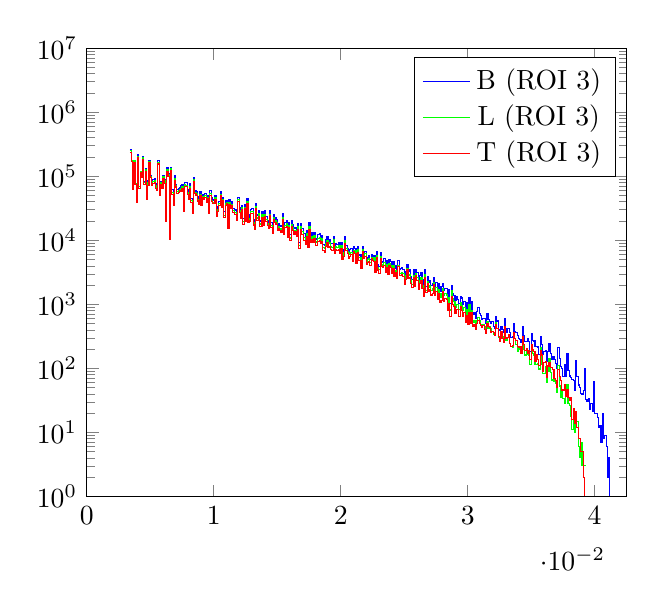
\begin{tikzpicture}

% Axis at [0.13 0.11 0.78 0.81]
\begin{semilogyaxis}[
axis on top,
xmin=0, xmax=0.0425,
ymin=1, ymax=1e+007,
%title={ROI 3},
legend entries={%
	B (ROI 3),%
	L (ROI 3),%
	T (ROI 3)}
]

\addplot [
color=blue,
solid
]coordinates{
 (0.0034,0) (0.0034,261785) (0.0034,261785) (0.0035,261785) (0.0035,171515) (0.0035,171515) (0.0036,171515) (0.0036,64140) (0.0036,64140) (0.0037,64140) (0.0037,178393) (0.0037,178393) (0.0038,178393) (0.0038,75348) (0.0038,75348) (0.0039,75348) (0.0039,46382) (0.0039,46382) (0.004,46382) (0.004,215725) (0.004,215725) (0.0041,215725) (0.0041,70020) (0.0041,70020) (0.0042,70020) (0.0042,119131) (0.0042,119131) (0.0043,119131) (0.0043,106518) (0.0043,106518) (0.0044,106518) (0.0044,205464) (0.0044,205464) (0.0045,205464) (0.0045,81381) (0.0045,81381) (0.0046,81381) (0.0046,132090) (0.0046,132090) (0.0047,132090) (0.0047,46500) (0.0047,46500) (0.0048,46500) (0.0048,86882) (0.0048,86882) (0.0049,86882) (0.0049,177449) (0.0049,177449) (0.005,177449) (0.005,104384) (0.005,104384) (0.0051,104384) (0.0051,79704) (0.0051,79704) (0.0052,79704) (0.0052,88134) (0.0052,88134) (0.0053,88134) (0.0053,91390) (0.0053,91390) (0.0054,91390) (0.0054,76156) (0.0054,76156) (0.0055,76156) (0.0055,67375) (0.0055,67375) (0.0056,67375) (0.0056,175138) (0.0056,175138) (0.0057,175138) (0.0057,56787) (0.0057,56787) (0.0058,56787) (0.0058,83486) (0.0058,83486) (0.0059,83486) (0.0059,76929) (0.0059,76929) (0.006,76929) (0.006,104060) (0.006,104060) (0.0061,104060) (0.0061,89587) (0.0061,89587) (0.0062,89587) (0.0062,24366) (0.0062,24366) (0.0063,24366) (0.0063,135688) (0.0063,135688) (0.0064,135688) (0.0064,111384) (0.0064,111384) (0.0065,111384) (0.0065,12855) (0.0065,12855) (0.0066,12855) (0.0066,138682) (0.0066,138682) (0.0067,138682) (0.0067,61809) (0.0067,61809) (0.0068,61809) (0.0068,44046) (0.0068,44046) (0.0069,44046) (0.0069,101518) (0.0069,101518) (0.007,101518) (0.007,75075) (0.007,75075) (0.0071,75075) (0.0071,62390) (0.0071,62390) (0.0072,62390) (0.0072,64998) (0.0072,64998) (0.0073,64998) (0.0073,67452) (0.0073,67452) (0.0074,67452) (0.0074,70334) (0.0074,70334) (0.0075,70334) (0.0075,75439) (0.0075,75439) (0.0076,75439) (0.0076,32535) (0.0076,32535) (0.0077,32535) (0.0077,79527) (0.0077,79527) (0.0078,79527) (0.0078,79109) (0.0078,79109) (0.0079,79109) (0.0079,61326) (0.0079,61326) (0.008,61326) (0.008,49543) (0.008,49543) (0.0081,49543) (0.0081,76006) (0.0081,76006) (0.0082,76006) (0.0082,45404) (0.0082,45404) (0.0083,45404) (0.0083,30199) (0.0083,30199) (0.0084,30199) (0.0084,96990) (0.0084,96990) (0.0085,96990) (0.0085,59335) (0.0085,59335) (0.0086,59335) (0.0086,57673) (0.0086,57673) (0.0087,57673) (0.0087,47603) (0.0087,47603) (0.0088,47603) (0.0088,42628) (0.0088,42628) (0.0089,42628) (0.0089,56988) (0.0089,56988) (0.009,56988) (0.009,41656) (0.009,41656) (0.0091,41656) (0.0091,52682) (0.0091,52682) (0.0092,52682) (0.0092,47187) (0.0092,47187) (0.0093,47187) (0.0093,54647) (0.0093,54647) (0.0094,54647) (0.0094,44404) (0.0094,44404) (0.0095,44404) (0.0095,50761) (0.0095,50761) (0.0096,50761) (0.0096,30337) (0.0096,30337) (0.0097,30337) (0.0097,59373) (0.0097,59373) (0.0098,59373) (0.0098,46057) (0.0098,46057) (0.0099,46057) (0.0099,42555) (0.0099,42555) (0.01,42555) (0.01,43013) (0.01,43013) (0.0101,43013) (0.0101,49493) (0.0101,49493) (0.0102,49493) (0.0102,27597) (0.0102,27597) (0.0103,27597) (0.0103,33162) (0.0103,33162) (0.0104,33162) (0.0104,40629) (0.0104,40629) (0.0105,40629) (0.0105,57212) (0.0105,57212) (0.0106,57212) (0.0106,37835) (0.0106,37835) (0.0107,37835) (0.0107,46461) (0.0107,46461) (0.0108,46461) (0.0108,27856) (0.0108,27856) (0.0109,27856) (0.0109,41149) (0.0109,41149) (0.011,41149) (0.011,42440) (0.011,42440) (0.0111,42440) (0.0111,18192) (0.0111,18192) (0.0112,18192) (0.0112,43305) (0.0112,43305) (0.0113,43305) (0.0113,37162) (0.0113,37162) (0.0114,37162) (0.0114,40000) (0.0114,40000) (0.0115,40000) (0.0115,31385) (0.0115,31385) (0.0116,31385) (0.0116,29331) (0.0116,29331) (0.0117,29331) (0.0117,30012) (0.0117,30012) (0.0118,30012) (0.0118,25089) (0.0118,25089) (0.0119,25089) (0.0119,47228) (0.0119,47228) (0.012,47228) (0.012,32020) (0.012,32020) (0.0121,32020) (0.0121,25085) (0.0121,25085) (0.0122,25085) (0.0122,35199) (0.0122,35199) (0.0123,35199) (0.0123,22062) (0.0123,22062) (0.0124,22062) (0.0124,36263) (0.0124,36263) (0.0125,36263) (0.0125,24485) (0.0125,24485) (0.0126,24485) (0.0126,44071) (0.0126,44071) (0.0127,44071) (0.0127,22324) (0.0127,22324) (0.0128,22324) (0.0128,25072) (0.0128,25072) (0.0129,25072) (0.0129,30631) (0.0129,30631) (0.013,30631) (0.013,30923) (0.013,30923) (0.0131,30923) (0.0131,21212) (0.0131,21212) (0.0132,21212) (0.0132,17798) (0.0132,17798) (0.0133,17798) (0.0133,37787) (0.0133,37787) (0.0134,37787) (0.0134,24807) (0.0134,24807) (0.0135,24807) (0.0135,28626) (0.0135,28626) (0.0136,28626) (0.0136,19411) (0.0136,19411) (0.0137,19411) (0.0137,20703) (0.0137,20703) (0.0138,20703) (0.0138,27951) (0.0138,27951) (0.0139,27951) (0.0139,21149) (0.0139,21149) (0.014,21149) (0.014,28650) (0.014,28650) (0.0141,28650) (0.0141,23865) (0.0141,23865) (0.0142,23865) (0.0142,20089) (0.0142,20089) (0.0143,20089) (0.0143,18758) (0.0143,18758) (0.0144,18758) (0.0144,28718) (0.0144,28718) (0.0145,28718) (0.0145,19216) (0.0145,19216) (0.0146,19216) (0.0146,15872) (0.0146,15872) (0.0147,15872) (0.0147,25443) (0.0147,25443) (0.0148,25443) (0.0148,22819) (0.0148,22819) (0.0149,22819) (0.0149,20878) (0.0149,20878) (0.015,20878) (0.015,17260) (0.015,17260) (0.0151,17260) (0.0151,18362) (0.0151,18362) (0.0152,18362) (0.0152,17057) (0.0152,17057) (0.0153,17057) (0.0153,16363) (0.0153,16363) (0.0154,16363) (0.0154,26002) (0.0154,26002) (0.0155,26002) (0.0155,14295) (0.0155,14295) (0.0156,14295) (0.0156,18841) (0.0156,18841) (0.0157,18841) (0.0157,20397) (0.0157,20397) (0.0158,20397) (0.0158,13500) (0.0158,13500) (0.0159,13500) (0.0159,19034) (0.0159,19034) (0.016,19034) (0.016,12174) (0.016,12174) (0.0161,12174) (0.0161,20153) (0.0161,20153) (0.0162,20153) (0.0162,17732) (0.0162,17732) (0.0163,17732) (0.0163,15175) (0.0163,15175) (0.0164,15175) (0.0164,16044) (0.0164,16044) (0.0165,16044) (0.0165,14214) (0.0165,14214) (0.0166,14214) (0.0166,18154) (0.0166,18154) (0.0167,18154) (0.0167,9192) (0.0167,9192) (0.0168,9192) (0.0168,18556) (0.0168,18556) (0.0169,18556) (0.0169,15243) (0.0169,15243) (0.017,15243) (0.017,15390) (0.017,15390) (0.0171,15390) (0.0171,12581) (0.0171,12581) (0.0172,12581) (0.0172,11097) (0.0172,11097) (0.0173,11097) (0.0173,14231) (0.0173,14231) (0.0174,14231) (0.0174,10018) (0.0174,10018) (0.0175,10018) (0.0175,18799) (0.0175,18799) (0.0176,18799) (0.0176,11256) (0.0176,11256) (0.0177,11256) (0.0177,13003) (0.0177,13003) (0.0178,13003) (0.0178,11939) (0.0178,11939) (0.0179,11939) (0.0179,13407) (0.0179,13407) (0.018,13407) (0.018,10466) (0.018,10466) (0.0181,10466) (0.0181,10704) (0.0181,10704) (0.0182,10704) (0.0182,12124) (0.0182,12124) (0.0183,12124) (0.0183,12615) (0.0183,12615) (0.0184,12615) (0.0184,11104) (0.0184,11104) (0.0185,11104) (0.0185,11889) (0.0185,11889) (0.0186,11889) (0.0186,8671) (0.0186,8671) (0.0187,8671) (0.0187,8305) (0.0187,8305) (0.0188,8305) (0.0188,10360) (0.0188,10360) (0.0189,10360) (0.0189,11524) (0.0189,11524) (0.019,11524) (0.019,9677) (0.019,9677) (0.0191,9677) (0.0191,10285) (0.0191,10285) (0.0192,10285) (0.0192,8863) (0.0192,8863) (0.0193,8863) (0.0193,8833) (0.0193,8833) (0.0194,8833) (0.0194,11615) (0.0194,11615) (0.0195,11615) (0.0195,7563) (0.0195,7563) (0.0196,7563) (0.0196,9011) (0.0196,9011) (0.0197,9011) (0.0197,8680) (0.0197,8680) (0.0198,8680) (0.0198,9346) (0.0198,9346) (0.0199,9346) (0.0199,7598) (0.0199,7598) (0.02,7598) (0.02,9368) (0.02,9368) (0.0201,9368) (0.0201,6243) (0.0201,6243) (0.0202,6243) (0.0202,7097) (0.0202,7097) (0.0203,7097) (0.0203,11333) (0.0203,11333) (0.0204,11333) (0.0204,8357) (0.0204,8357) (0.0205,8357) (0.0205,7548) (0.0205,7548) (0.0206,7548) (0.0206,6573) (0.0206,6573) (0.0207,6573) (0.0207,7110) (0.0207,7110) (0.0208,7110) (0.0208,7435) (0.0208,7435) (0.0209,7435) (0.0209,5902) (0.0209,5902) (0.021,5902) (0.021,7910) (0.021,7910) (0.0211,7910) (0.0211,7553) (0.0211,7553) (0.0212,7553) (0.0212,5328) (0.0212,5328) (0.0213,5328) (0.0213,7972) (0.0213,7972) (0.0214,7972) (0.0214,6013) (0.0214,6013) (0.0215,6013) (0.0215,5895) (0.0215,5895) (0.0216,5895) (0.0216,4557) (0.0216,4557) (0.0217,4557) (0.0217,8066) (0.0217,8066) (0.0218,8066) (0.0218,6138) (0.0218,6138) (0.0219,6138) (0.0219,6652) (0.0219,6652) (0.022,6652) (0.022,5074) (0.022,5074) (0.0221,5074) (0.0221,5389) (0.0221,5389) (0.0222,5389) (0.0222,5880) (0.0222,5880) (0.0223,5880) (0.0223,5021) (0.0223,5021) (0.0224,5021) (0.0224,5965) (0.0224,5965) (0.0225,5965) (0.0225,5697) (0.0225,5697) (0.0226,5697) (0.0226,5874) (0.0226,5874) (0.0227,5874) (0.0227,3867) (0.0227,3867) (0.0228,3867) (0.0228,6625) (0.0228,6625) (0.0229,6625) (0.0229,4173) (0.0229,4173) (0.023,4173) (0.023,3932) (0.023,3932) (0.0231,3932) (0.0231,6363) (0.0231,6363) (0.0232,6363) (0.0232,4695) (0.0232,4695) (0.0233,4695) (0.0233,4442) (0.0233,4442) (0.0234,4442) (0.0234,5116) (0.0234,5116) (0.0235,5116) (0.0235,4022) (0.0235,4022) (0.0236,4022) (0.0236,4794) (0.0236,4794) (0.0237,4794) (0.0237,3734) (0.0237,3734) (0.0238,3734) (0.0238,4991) (0.0238,4991) (0.0239,4991) (0.0239,4625) (0.0239,4625) (0.024,4625) (0.024,3698) (0.024,3698) (0.0241,3698) (0.0241,4677) (0.0241,4677) (0.0242,4677) (0.0242,3644) (0.0242,3644) (0.0243,3644) (0.0243,3979) (0.0243,3979) (0.0244,3979) (0.0244,3279) (0.0244,3279) (0.0245,3279) (0.0245,4809) (0.0245,4809) (0.0246,4809) (0.0246,3543) (0.0246,3543) (0.0247,3543) (0.0247,3674) (0.0247,3674) (0.0248,3674) (0.0248,3706) (0.0248,3706) (0.0249,3706) (0.0249,3525) (0.0249,3525) (0.025,3525) (0.025,2748) (0.025,2748) (0.0251,2748) (0.0251,3289) (0.0251,3289) (0.0252,3289) (0.0252,4250) (0.0252,4250) (0.0253,4250) (0.0253,3251) (0.0253,3251) (0.0254,3251) (0.0254,3445) (0.0254,3445) (0.0255,3445) (0.0255,2732) (0.0255,2732) (0.0256,2732) (0.0256,2426) (0.0256,2426) (0.0257,2426) (0.0257,3442) (0.0257,3442) (0.0258,3442) (0.0258,2627) (0.0258,2627) (0.0259,2627) (0.0259,3505) (0.0259,3505) (0.026,3505) (0.026,3120) (0.026,3120) (0.0261,3120) (0.0261,2118) (0.0261,2118) (0.0262,2118) (0.0262,2836) (0.0262,2836) (0.0263,2836) (0.0263,3139) (0.0263,3139) (0.0264,3139) (0.0264,2398) (0.0264,2398) (0.0265,2398) (0.0265,1775) (0.0265,1775) (0.0266,1775) (0.0266,3440) (0.0266,3440) (0.0267,3440) (0.0267,1910) (0.0267,1910) (0.0268,1910) (0.0268,2712) (0.0268,2712) (0.0269,2712) (0.0269,2195) (0.0269,2195) (0.027,2195) (0.027,2388) (0.027,2388) (0.0271,2388) (0.0271,1999) (0.0271,1999) (0.0272,1999) (0.0272,2142) (0.0272,2142) (0.0273,2142) (0.0273,2635) (0.0273,2635) (0.0274,2635) (0.0274,1909) (0.0274,1909) (0.0275,1909) (0.0275,2227) (0.0275,2227) (0.0276,2227) (0.0276,1764) (0.0276,1764) (0.0277,1764) (0.0277,2096) (0.0277,2096) (0.0278,2096) (0.0278,1583) (0.0278,1583) (0.0279,1583) (0.0279,1873) (0.0279,1873) (0.028,1873) (0.028,2144) (0.028,2144) (0.0281,2144) (0.0281,1640) (0.0281,1640) (0.0282,1640) (0.0282,1786) (0.0282,1786) (0.0283,1786) (0.0283,1744) (0.0283,1744) (0.0284,1744) (0.0284,1223) (0.0284,1223) (0.0285,1223) (0.0285,1674) (0.0285,1674) (0.0286,1674) (0.0286,1025) (0.0286,1025) (0.0287,1025) (0.0287,1962) (0.0287,1962) (0.0288,1962) (0.0288,1473) (0.0288,1473) (0.0289,1473) (0.0289,1370) (0.0289,1370) (0.029,1370) (0.029,1137) (0.029,1137) (0.0291,1137) (0.0291,1334) (0.0291,1334) (0.0292,1334) (0.0292,1202) (0.0292,1202) (0.0293,1202) (0.0293,1017) (0.0293,1017) (0.0294,1017) (0.0294,1327) (0.0294,1327) (0.0295,1327) (0.0295,1254) (0.0295,1254) (0.0296,1254) (0.0296,992) (0.0296,992) (0.0297,992) (0.0297,1121) (0.0297,1121) (0.0298,1121) (0.0298,774) (0.0298,774) (0.0299,774) (0.0299,1052) (0.0299,1052) (0.03,1052) (0.03,738) (0.03,738) (0.0301,738) (0.0301,1259) (0.0301,1259) (0.0302,1259) (0.0302,758) (0.0302,758) (0.0303,758) (0.0303,1115) (0.0303,1115) (0.0304,1115) (0.0304,690) (0.0304,690) (0.0305,690) (0.0305,750) (0.0305,750) (0.0306,750) (0.0306,598) (0.0306,598) (0.0307,598) (0.0307,766) (0.0307,766) (0.0308,766) (0.0308,904) (0.0308,904) (0.0309,904) (0.0309,721) (0.0309,721) (0.031,721) (0.031,676) (0.031,676) (0.0311,676) (0.0311,577) (0.0311,577) (0.0312,577) (0.0312,603) (0.0312,603) (0.0313,603) (0.0313,597) (0.0313,597) (0.0314,597) (0.0314,504) (0.0314,504) (0.0315,504) (0.0315,714) (0.0315,714) (0.0316,714) (0.0316,575) (0.0316,575) (0.0317,575) (0.0317,532) (0.0317,532) (0.0318,532) (0.0318,504) (0.0318,504) (0.0319,504) (0.0319,538) (0.0319,538) (0.032,538) (0.032,448) (0.032,448) (0.0321,448) (0.0321,420) (0.0321,420) (0.0322,420) (0.0322,649) (0.0322,649) (0.0323,649) (0.0323,550) (0.0323,550) (0.0324,550) (0.0324,407) (0.0324,407) (0.0325,407) (0.0325,390) (0.0325,390) (0.0326,390) (0.0326,453) (0.0326,453) (0.0327,453) (0.0327,399) (0.0327,399) (0.0328,399) (0.0328,362) (0.0328,362) (0.0329,362) (0.0329,593) (0.0329,593) (0.033,593) (0.033,363) (0.033,363) (0.0331,363) (0.0331,417) (0.0331,417) (0.0332,417) (0.0332,426) (0.0332,426) (0.0333,426) (0.0333,358) (0.0333,358) (0.0334,358) (0.0334,303) (0.0334,303) (0.0335,303) (0.0335,319) (0.0335,319) (0.0336,319) (0.0336,497) (0.0336,497) (0.0337,497) (0.0337,370) (0.0337,370) (0.0338,370) (0.0338,367) (0.0338,367) (0.0339,367) (0.0339,323) (0.0339,323) (0.034,323) (0.034,295) (0.034,295) (0.0341,295) (0.0341,285) (0.0341,285) (0.0342,285) (0.0342,256) (0.0342,256) (0.0343,256) (0.0343,456) (0.0343,456) (0.0344,456) (0.0344,326) (0.0344,326) (0.0345,326) (0.0345,262) (0.0345,262) (0.0346,262) (0.0346,262) (0.0346,262) (0.0347,262) (0.0347,290) (0.0347,290) (0.0348,290) (0.0348,263) (0.0348,263) (0.0349,263) (0.0349,183) (0.0349,183) (0.035,183) (0.035,350) (0.035,350) (0.0351,350) (0.0351,274) (0.0351,274) (0.0352,274) (0.0352,268) (0.0352,268) (0.0353,268) (0.0353,217) (0.0353,217) (0.0354,217) (0.0354,218) (0.0354,218) (0.0355,218) (0.0355,216) (0.0355,216) (0.0356,216) (0.0356,166) (0.0356,166) (0.0357,166) (0.0357,310) (0.0357,310) (0.0358,310) (0.0358,237) (0.0358,237) (0.0359,237) (0.0359,164) (0.0359,164) (0.036,164) (0.036,182) (0.036,182) (0.0361,182) (0.0361,191) (0.0361,191) (0.0362,191) (0.0362,129) (0.0362,129) (0.0363,129) (0.0363,183) (0.0363,183) (0.0364,183) (0.0364,243) (0.0364,243) (0.0365,243) (0.0365,169) (0.0365,169) (0.0366,169) (0.0366,139) (0.0366,139) (0.0367,139) (0.0367,152) (0.0367,152) (0.0368,152) (0.0368,136) (0.0368,136) (0.0369,136) (0.0369,118) (0.0369,118) (0.037,118) (0.037,101) (0.037,101) (0.0371,101) (0.0371,214) (0.0371,214) (0.0372,214) (0.0372,145) (0.0372,145) (0.0373,145) (0.0373,108) (0.0373,108) (0.0374,108) (0.0374,99) (0.0374,99) (0.0375,99) (0.0375,75) (0.0375,75) (0.0376,75) (0.0376,116) (0.0376,116) (0.0377,116) (0.0377,75) (0.0377,75) (0.0378,75) (0.0378,173) (0.0378,173) (0.0379,173) (0.0379,93) (0.0379,93) (0.038,93) (0.038,76) (0.038,76) (0.0381,76) (0.0381,72) (0.0381,72) (0.0382,72) (0.0382,67) (0.0382,67) (0.0383,67) (0.0383,65) (0.0383,65) (0.0384,65) (0.0384,46) (0.0384,46) (0.0385,46) (0.0385,133) (0.0385,133) (0.0386,133) (0.0386,74) (0.0386,74) (0.0387,74) (0.0387,55) (0.0387,55) (0.0388,55) (0.0388,50) (0.0388,50) (0.0389,50) (0.0389,40) (0.0389,40) (0.039,40) (0.039,39) (0.039,39) (0.0391,39) (0.0391,45) (0.0391,45) (0.0392,45) (0.0392,101) (0.0392,101) (0.0393,101) (0.0393,33) (0.0393,33) (0.0394,33) (0.0394,31) (0.0394,31) (0.0395,31) (0.0395,34) (0.0395,34) (0.0396,34) (0.0396,23) (0.0396,23) (0.0397,23) (0.0397,28) (0.0397,28) (0.0398,28) (0.0398,21) (0.0398,21) (0.0399,21) (0.0399,62) (0.0399,62) (0.04,62) (0.04,20) (0.04,20) (0.0401,20) (0.0401,20) (0.0401,20) (0.0402,20) (0.0402,17) (0.0402,17) (0.0403,17) (0.0403,12) (0.0403,12) (0.0404,12) (0.0404,13) (0.0404,13) (0.0405,13) (0.0405,7) (0.0405,7) (0.0406,7) (0.0406,20) (0.0406,20) (0.0407,20) (0.0407,8) (0.0407,8) (0.0408,8) (0.0408,9) (0.0408,9) (0.0409,9) (0.0409,6) (0.0409,6) (0.041,6) (0.041,2) (0.041,2) (0.0411,2) (0.0411,4) (0.0411,4) (0.0412,4) (0.0412,1)
};

\addplot [
color=green,
solid
]coordinates{
 (0.0034,0) (0.0034,248612) (0.0034,248612) (0.0035,248612) (0.0035,173238) (0.0035,173238) (0.0036,173238) (0.0036,64514) (0.0036,64514) (0.0037,64514) (0.0037,173352) (0.0037,173352) (0.0038,173352) (0.0038,76196) (0.0038,76196) (0.0039,76196) (0.0039,42829) (0.0039,42829) (0.004,42829) (0.004,206073) (0.004,206073) (0.0041,206073) (0.0041,68752) (0.0041,68752) (0.0042,68752) (0.0042,116705) (0.0042,116705) (0.0043,116705) (0.0043,102908) (0.0043,102908) (0.0044,102908) (0.0044,195726) (0.0044,195726) (0.0045,195726) (0.0045,80247) (0.0045,80247) (0.0046,80247) (0.0046,125482) (0.0046,125482) (0.0047,125482) (0.0047,45503) (0.0047,45503) (0.0048,45503) (0.0048,78405) (0.0048,78405) (0.0049,78405) (0.0049,170517) (0.0049,170517) (0.005,170517) (0.005,100461) (0.005,100461) (0.0051,100461) (0.0051,76984) (0.0051,76984) (0.0052,76984) (0.0052,82834) (0.0052,82834) (0.0053,82834) (0.0053,85003) (0.0053,85003) (0.0054,85003) (0.0054,70381) (0.0054,70381) (0.0055,70381) (0.0055,65105) (0.0055,65105) (0.0056,65105) (0.0056,163806) (0.0056,163806) (0.0057,163806) (0.0057,53569) (0.0057,53569) (0.0058,53569) (0.0058,79374) (0.0058,79374) (0.0059,79374) (0.0059,69589) (0.0059,69589) (0.006,69589) (0.006,97928) (0.006,97928) (0.0061,97928) (0.0061,84273) (0.0061,84273) (0.0062,84273) (0.0062,21566) (0.0062,21566) (0.0063,21566) (0.0063,125043) (0.0063,125043) (0.0064,125043) (0.0064,104632) (0.0064,104632) (0.0065,104632) (0.0065,11430) (0.0065,11430) (0.0066,11430) (0.0066,130152) (0.0066,130152) (0.0067,130152) (0.0067,55974) (0.0067,55974) (0.0068,55974) (0.0068,39190) (0.0068,39190) (0.0069,39190) (0.0069,92900) (0.0069,92900) (0.007,92900) (0.007,71151) (0.007,71151) (0.0071,71151) (0.0071,57434) (0.0071,57434) (0.0072,57434) (0.0072,59605) (0.0072,59605) (0.0073,59605) (0.0073,62875) (0.0073,62875) (0.0074,62875) (0.0074,63452) (0.0074,63452) (0.0075,63452) (0.0075,69555) (0.0075,69555) (0.0076,69555) (0.0076,29814) (0.0076,29814) (0.0077,29814) (0.0077,72913) (0.0077,72913) (0.0078,72913) (0.0078,72832) (0.0078,72832) (0.0079,72832) (0.0079,55683) (0.0079,55683) (0.008,55683) (0.008,45521) (0.008,45521) (0.0081,45521) (0.0081,69903) (0.0081,69903) (0.0082,69903) (0.0082,41311) (0.0082,41311) (0.0083,41311) (0.0083,27713) (0.0083,27713) (0.0084,27713) (0.0084,87376) (0.0084,87376) (0.0085,87376) (0.0085,55895) (0.0085,55895) (0.0086,55895) (0.0086,53190) (0.0086,53190) (0.0087,53190) (0.0087,43470) (0.0087,43470) (0.0088,43470) (0.0088,38010) (0.0088,38010) (0.0089,38010) (0.0089,52362) (0.0089,52362) (0.009,52362) (0.009,37847) (0.009,37847) (0.0091,37847) (0.0091,48359) (0.0091,48359) (0.0092,48359) (0.0092,44103) (0.0092,44103) (0.0093,44103) (0.0093,49445) (0.0093,49445) (0.0094,49445) (0.0094,40992) (0.0094,40992) (0.0095,40992) (0.0095,47005) (0.0095,47005) (0.0096,47005) (0.0096,27670) (0.0096,27670) (0.0097,27670) (0.0097,54007) (0.0097,54007) (0.0098,54007) (0.0098,42212) (0.0098,42212) (0.0099,42212) (0.0099,39295) (0.0099,39295) (0.01,39295) (0.01,39456) (0.01,39456) (0.0101,39456) (0.0101,45981) (0.0101,45981) (0.0102,45981) (0.0102,25139) (0.0102,25139) (0.0103,25139) (0.0103,30049) (0.0103,30049) (0.0104,30049) (0.0104,37081) (0.0104,37081) (0.0105,37081) (0.0105,52431) (0.0105,52431) (0.0106,52431) (0.0106,35267) (0.0106,35267) (0.0107,35267) (0.0107,43412) (0.0107,43412) (0.0108,43412) (0.0108,24768) (0.0108,24768) (0.0109,24768) (0.0109,38077) (0.0109,38077) (0.011,38077) (0.011,39323) (0.011,39323) (0.0111,39323) (0.0111,16698) (0.0111,16698) (0.0112,16698) (0.0112,39399) (0.0112,39399) (0.0113,39399) (0.0113,34418) (0.0113,34418) (0.0114,34418) (0.0114,36579) (0.0114,36579) (0.0115,36579) (0.0115,29135) (0.0115,29135) (0.0116,29135) (0.0116,27206) (0.0116,27206) (0.0117,27206) (0.0117,27317) (0.0117,27317) (0.0118,27317) (0.0118,22672) (0.0118,22672) (0.0119,22672) (0.0119,43030) (0.0119,43030) (0.012,43030) (0.012,29578) (0.012,29578) (0.0121,29578) (0.0121,23093) (0.0121,23093) (0.0122,23093) (0.0122,32274) (0.0122,32274) (0.0123,32274) (0.0123,19571) (0.0123,19571) (0.0124,19571) (0.0124,32995) (0.0124,32995) (0.0125,32995) (0.0125,22153) (0.0125,22153) (0.0126,22153) (0.0126,39969) (0.0126,39969) (0.0127,39969) (0.0127,20483) (0.0127,20483) (0.0128,20483) (0.0128,22168) (0.0128,22168) (0.0129,22168) (0.0129,27886) (0.0129,27886) (0.013,27886) (0.013,27917) (0.013,27917) (0.0131,27917) (0.0131,19128) (0.0131,19128) (0.0132,19128) (0.0132,16022) (0.0132,16022) (0.0133,16022) (0.0133,33478) (0.0133,33478) (0.0134,33478) (0.0134,22290) (0.0134,22290) (0.0135,22290) (0.0135,25793) (0.0135,25793) (0.0136,25793) (0.0136,17567) (0.0136,17567) (0.0137,17567) (0.0137,18173) (0.0137,18173) (0.0138,18173) (0.0138,24836) (0.0138,24836) (0.0139,24836) (0.0139,18503) (0.0139,18503) (0.014,18503) (0.014,25510) (0.014,25510) (0.0141,25510) (0.0141,21385) (0.0141,21385) (0.0142,21385) (0.0142,18074) (0.0142,18074) (0.0143,18074) (0.0143,16718) (0.0143,16718) (0.0144,16718) (0.0144,25483) (0.0144,25483) (0.0145,25483) (0.0145,17089) (0.0145,17089) (0.0146,17089) (0.0146,14011) (0.0146,14011) (0.0147,14011) (0.0147,22886) (0.0147,22886) (0.0148,22886) (0.0148,20276) (0.0148,20276) (0.0149,20276) (0.0149,18610) (0.0149,18610) (0.015,18610) (0.015,15624) (0.015,15624) (0.0151,15624) (0.0151,16442) (0.0151,16442) (0.0152,16442) (0.0152,15353) (0.0152,15353) (0.0153,15353) (0.0153,14304) (0.0153,14304) (0.0154,14304) (0.0154,22901) (0.0154,22901) (0.0155,22901) (0.0155,13053) (0.0155,13053) (0.0156,13053) (0.0156,17127) (0.0156,17127) (0.0157,17127) (0.0157,17952) (0.0157,17952) (0.0158,17952) (0.0158,12128) (0.0158,12128) (0.0159,12128) (0.0159,16990) (0.0159,16990) (0.016,16990) (0.016,10872) (0.016,10872) (0.0161,10872) (0.0161,17748) (0.0161,17748) (0.0162,17748) (0.0162,15901) (0.0162,15901) (0.0163,15901) (0.0163,13489) (0.0163,13489) (0.0164,13489) (0.0164,14449) (0.0164,14449) (0.0165,14449) (0.0165,12462) (0.0165,12462) (0.0166,12462) (0.0166,16171) (0.0166,16171) (0.0167,16171) (0.0167,8164) (0.0167,8164) (0.0168,8164) (0.0168,16101) (0.0168,16101) (0.0169,16101) (0.0169,13603) (0.0169,13603) (0.017,13603) (0.017,13587) (0.017,13587) (0.0171,13587) (0.0171,11170) (0.0171,11170) (0.0172,11170) (0.0172,9853) (0.0172,9853) (0.0173,9853) (0.0173,12542) (0.0173,12542) (0.0174,12542) (0.0174,8662) (0.0174,8662) (0.0175,8662) (0.0175,16547) (0.0175,16547) (0.0176,16547) (0.0176,10059) (0.0176,10059) (0.0177,10059) (0.0177,11448) (0.0177,11448) (0.0178,11448) (0.0178,10528) (0.0178,10528) (0.0179,10528) (0.0179,12039) (0.0179,12039) (0.018,12039) (0.018,9195) (0.018,9195) (0.0181,9195) (0.0181,9462) (0.0181,9462) (0.0182,9462) (0.0182,10644) (0.0182,10644) (0.0183,10644) (0.0183,11214) (0.0183,11214) (0.0184,11214) (0.0184,9833) (0.0184,9833) (0.0185,9833) (0.0185,10487) (0.0185,10487) (0.0186,10487) (0.0186,7765) (0.0186,7765) (0.0187,7765) (0.0187,7525) (0.0187,7525) (0.0188,7525) (0.0188,9007) (0.0188,9007) (0.0189,9007) (0.0189,9981) (0.0189,9981) (0.019,9981) (0.019,8775) (0.019,8775) (0.0191,8775) (0.0191,9084) (0.0191,9084) (0.0192,9084) (0.0192,7951) (0.0192,7951) (0.0193,7951) (0.0193,7821) (0.0193,7821) (0.0194,7821) (0.0194,10183) (0.0194,10183) (0.0195,10183) (0.0195,6857) (0.0195,6857) (0.0196,6857) (0.0196,7891) (0.0196,7891) (0.0197,7891) (0.0197,7671) (0.0197,7671) (0.0198,7671) (0.0198,8210) (0.0198,8210) (0.0199,8210) (0.0199,6943) (0.0199,6943) (0.02,6943) (0.02,8234) (0.02,8234) (0.0201,8234) (0.0201,5559) (0.0201,5559) (0.0202,5559) (0.0202,6416) (0.0202,6416) (0.0203,6416) (0.0203,9753) (0.0203,9753) (0.0204,9753) (0.0204,7540) (0.0204,7540) (0.0205,7540) (0.0205,6766) (0.0205,6766) (0.0206,6766) (0.0206,5972) (0.0206,5972) (0.0207,5972) (0.0207,6337) (0.0207,6337) (0.0208,6337) (0.0208,6516) (0.0208,6516) (0.0209,6516) (0.0209,5271) (0.0209,5271) (0.021,5271) (0.021,6977) (0.021,6977) (0.0211,6977) (0.0211,6816) (0.0211,6816) (0.0212,6816) (0.0212,4804) (0.0212,4804) (0.0213,4804) (0.0213,7196) (0.0213,7196) (0.0214,7196) (0.0214,5391) (0.0214,5391) (0.0215,5391) (0.0215,5344) (0.0215,5344) (0.0216,5344) (0.0216,4148) (0.0216,4148) (0.0217,4148) (0.0217,7146) (0.0217,7146) (0.0218,7146) (0.0218,5523) (0.0218,5523) (0.0219,5523) (0.0219,6167) (0.0219,6167) (0.022,6167) (0.022,4483) (0.022,4483) (0.0221,4483) (0.0221,5014) (0.0221,5014) (0.0222,5014) (0.0222,5234) (0.0222,5234) (0.0223,5234) (0.0223,4462) (0.0223,4462) (0.0224,4462) (0.0224,5453) (0.0224,5453) (0.0225,5453) (0.0225,5075) (0.0225,5075) (0.0226,5075) (0.0226,5338) (0.0226,5338) (0.0227,5338) (0.0227,3465) (0.0227,3465) (0.0228,3465) (0.0228,5880) (0.0228,5880) (0.0229,5880) (0.0229,3693) (0.0229,3693) (0.023,3693) (0.023,3540) (0.023,3540) (0.0231,3540) (0.0231,5641) (0.0231,5641) (0.0232,5641) (0.0232,4180) (0.0232,4180) (0.0233,4180) (0.0233,3881) (0.0233,3881) (0.0234,3881) (0.0234,4518) (0.0234,4518) (0.0235,4518) (0.0235,3530) (0.0235,3530) (0.0236,3530) (0.0236,4188) (0.0236,4188) (0.0237,4188) (0.0237,3126) (0.0237,3126) (0.0238,3126) (0.0238,4370) (0.0238,4370) (0.0239,4370) (0.0239,4064) (0.0239,4064) (0.024,4064) (0.024,3166) (0.024,3166) (0.0241,3166) (0.0241,4019) (0.0241,4019) (0.0242,4019) (0.0242,2931) (0.0242,2931) (0.0243,2931) (0.0243,3372) (0.0243,3372) (0.0244,3372) (0.0244,2795) (0.0244,2795) (0.0245,2795) (0.0245,4061) (0.0245,4061) (0.0246,4061) (0.0246,3039) (0.0246,3039) (0.0247,3039) (0.0247,3056) (0.0247,3056) (0.0248,3056) (0.0248,3088) (0.0248,3088) (0.0249,3088) (0.0249,2987) (0.0249,2987) (0.025,2987) (0.025,2287) (0.025,2287) (0.0251,2287) (0.0251,2803) (0.0251,2803) (0.0252,2803) (0.0252,3562) (0.0252,3562) (0.0253,3562) (0.0253,2789) (0.0253,2789) (0.0254,2789) (0.0254,2888) (0.0254,2888) (0.0255,2888) (0.0255,2402) (0.0255,2402) (0.0256,2402) (0.0256,2011) (0.0256,2011) (0.0257,2011) (0.0257,2845) (0.0257,2845) (0.0258,2845) (0.0258,2167) (0.0258,2167) (0.0259,2167) (0.0259,3059) (0.0259,3059) (0.026,3059) (0.026,2635) (0.026,2635) (0.0261,2635) (0.0261,1881) (0.0261,1881) (0.0262,1881) (0.0262,2369) (0.0262,2369) (0.0263,2369) (0.0263,2639) (0.0263,2639) (0.0264,2639) (0.0264,1973) (0.0264,1973) (0.0265,1973) (0.0265,1516) (0.0265,1516) (0.0266,1516) (0.0266,2910) (0.0266,2910) (0.0267,2910) (0.0267,1648) (0.0267,1648) (0.0268,1648) (0.0268,2290) (0.0268,2290) (0.0269,2290) (0.0269,1865) (0.0269,1865) (0.027,1865) (0.027,1945) (0.027,1945) (0.0271,1945) (0.0271,1625) (0.0271,1625) (0.0272,1625) (0.0272,1736) (0.0272,1736) (0.0273,1736) (0.0273,2216) (0.0273,2216) (0.0274,2216) (0.0274,1554) (0.0274,1554) (0.0275,1554) (0.0275,1825) (0.0275,1825) (0.0276,1825) (0.0276,1394) (0.0276,1394) (0.0277,1394) (0.0277,1704) (0.0277,1704) (0.0278,1704) (0.0278,1276) (0.0278,1276) (0.0279,1276) (0.0279,1481) (0.0279,1481) (0.028,1481) (0.028,1782) (0.028,1782) (0.0281,1782) (0.0281,1364) (0.0281,1364) (0.0282,1364) (0.0282,1492) (0.0282,1492) (0.0283,1492) (0.0283,1400) (0.0283,1400) (0.0284,1400) (0.0284,1013) (0.0284,1013) (0.0285,1013) (0.0285,1298) (0.0285,1298) (0.0286,1298) (0.0286,816) (0.0286,816) (0.0287,816) (0.0287,1618) (0.0287,1618) (0.0288,1618) (0.0288,1213) (0.0288,1213) (0.0289,1213) (0.0289,1116) (0.0289,1116) (0.029,1116) (0.029,908) (0.029,908) (0.0291,908) (0.0291,991) (0.0291,991) (0.0292,991) (0.0292,996) (0.0292,996) (0.0293,996) (0.0293,833) (0.0293,833) (0.0294,833) (0.0294,1058) (0.0294,1058) (0.0295,1058) (0.0295,971) (0.0295,971) (0.0296,971) (0.0296,799) (0.0296,799) (0.0297,799) (0.0297,880) (0.0297,880) (0.0298,880) (0.0298,616) (0.0298,616) (0.0299,616) (0.0299,818) (0.0299,818) (0.03,818) (0.03,568) (0.03,568) (0.0301,568) (0.0301,975) (0.0301,975) (0.0302,975) (0.0302,586) (0.0302,586) (0.0303,586) (0.0303,803) (0.0303,803) (0.0304,803) (0.0304,523) (0.0304,523) (0.0305,523) (0.0305,559) (0.0305,559) (0.0306,559) (0.0306,459) (0.0306,459) (0.0307,459) (0.0307,567) (0.0307,567) (0.0308,567) (0.0308,632) (0.0308,632) (0.0309,632) (0.0309,565) (0.0309,565) (0.031,565) (0.031,482) (0.031,482) (0.0311,482) (0.0311,445) (0.0311,445) (0.0312,445) (0.0312,475) (0.0312,475) (0.0313,475) (0.0313,455) (0.0313,455) (0.0314,455) (0.0314,368) (0.0314,368) (0.0315,368) (0.0315,537) (0.0315,537) (0.0316,537) (0.0316,421) (0.0316,421) (0.0317,421) (0.0317,451) (0.0317,451) (0.0318,451) (0.0318,419) (0.0318,419) (0.0319,419) (0.0319,379) (0.0319,379) (0.032,379) (0.032,334) (0.032,334) (0.0321,334) (0.0321,351) (0.0321,351) (0.0322,351) (0.0322,512) (0.0322,512) (0.0323,512) (0.0323,419) (0.0323,419) (0.0324,419) (0.0324,308) (0.0324,308) (0.0325,308) (0.0325,280) (0.0325,280) (0.0326,280) (0.0326,354) (0.0326,354) (0.0327,354) (0.0327,313) (0.0327,313) (0.0328,313) (0.0328,269) (0.0328,269) (0.0329,269) (0.0329,426) (0.0329,426) (0.033,426) (0.033,274) (0.033,274) (0.0331,274) (0.0331,300) (0.0331,300) (0.0332,300) (0.0332,323) (0.0332,323) (0.0333,323) (0.0333,244) (0.0333,244) (0.0334,244) (0.0334,223) (0.0334,223) (0.0335,223) (0.0335,215) (0.0335,215) (0.0336,215) (0.0336,344) (0.0336,344) (0.0337,344) (0.0337,292) (0.0337,292) (0.0338,292) (0.0338,234) (0.0338,234) (0.0339,234) (0.0339,186) (0.0339,186) (0.034,186) (0.034,210) (0.034,210) (0.0341,210) (0.0341,199) (0.0341,199) (0.0342,199) (0.0342,188) (0.0342,188) (0.0343,188) (0.0343,295) (0.0343,295) (0.0344,295) (0.0344,198) (0.0344,198) (0.0345,198) (0.0345,162) (0.0345,162) (0.0346,162) (0.0346,182) (0.0346,182) (0.0347,182) (0.0347,164) (0.0347,164) (0.0348,164) (0.0348,159) (0.0348,159) (0.0349,159) (0.0349,115) (0.0349,115) (0.035,115) (0.035,223) (0.035,223) (0.0351,223) (0.0351,173) (0.0351,173) (0.0352,173) (0.0352,161) (0.0352,161) (0.0353,161) (0.0353,114) (0.0353,114) (0.0354,114) (0.0354,115) (0.0354,115) (0.0355,115) (0.0355,117) (0.0355,117) (0.0356,117) (0.0356,98) (0.0356,98) (0.0357,98) (0.0357,213) (0.0357,213) (0.0358,213) (0.0358,117) (0.0358,117) (0.0359,117) (0.0359,84) (0.0359,84) (0.036,84) (0.036,84) (0.036,84) (0.0361,84) (0.0361,107) (0.0361,107) (0.0362,107) (0.0362,60) (0.0362,60) (0.0363,60) (0.0363,91) (0.0363,91) (0.0364,91) (0.0364,140) (0.0364,140) (0.0365,140) (0.0365,87) (0.0365,87) (0.0366,87) (0.0366,65) (0.0366,65) (0.0367,65) (0.0367,67) (0.0367,67) (0.0368,67) (0.0368,62) (0.0368,62) (0.0369,62) (0.0369,59) (0.0369,59) (0.037,59) (0.037,42) (0.037,42) (0.0371,42) (0.0371,110) (0.0371,110) (0.0372,110) (0.0372,53) (0.0372,53) (0.0373,53) (0.0373,35) (0.0373,35) (0.0374,35) (0.0374,46) (0.0374,46) (0.0375,46) (0.0375,34) (0.0375,34) (0.0376,34) (0.0376,28) (0.0376,28) (0.0377,28) (0.0377,37) (0.0377,37) (0.0378,37) (0.0378,56) (0.0378,56) (0.0379,56) (0.0379,28) (0.0379,28) (0.038,28) (0.038,26) (0.038,26) (0.0381,26) (0.0381,18) (0.0381,18) (0.0382,18) (0.0382,11) (0.0382,11) (0.0383,11) (0.0383,20) (0.0383,20) (0.0384,20) (0.0384,10) (0.0384,10) (0.0385,10) (0.0385,18) (0.0385,18) (0.0386,18) (0.0386,15) (0.0386,15) (0.0387,15) (0.0387,6) (0.0387,6) (0.0388,6) (0.0388,4) (0.0388,4) (0.0389,4) (0.0389,7) (0.0389,7) (0.039,7) (0.039,3) (0.039,3) (0.0391,3) (0.0391,3) (0.0391,3) (0.0392,3) (0.0392,3) (0.0392,3) (0.0393,3) (0.0393,0)
};

\addplot [
color=red,
solid
]coordinates{
 (0.0034,0) (0.0034,237538) (0.0034,237538) (0.0035,237538) (0.0035,170425) (0.0035,170425) (0.0036,170425) (0.0036,62488) (0.0036,62488) (0.0037,62488) (0.0037,164909) (0.0037,164909) (0.0038,164909) (0.0038,74281) (0.0038,74281) (0.0039,74281) (0.0039,38720) (0.0039,38720) (0.004,38720) (0.004,193850) (0.004,193850) (0.0041,193850) (0.0041,65260) (0.0041,65260) (0.0042,65260) (0.0042,115725) (0.0042,115725) (0.0043,115725) (0.0043,96958) (0.0043,96958) (0.0044,96958) (0.0044,185116) (0.0044,185116) (0.0045,185116) (0.0045,74643) (0.0045,74643) (0.0046,74643) (0.0046,118126) (0.0046,118126) (0.0047,118126) (0.0047,43475) (0.0047,43475) (0.0048,43475) (0.0048,71037) (0.0048,71037) (0.0049,71037) (0.0049,163157) (0.0049,163157) (0.005,163157) (0.005,96295) (0.005,96295) (0.0051,96295) (0.0051,72694) (0.0051,72694) (0.0052,72694) (0.0052,76384) (0.0052,76384) (0.0053,76384) (0.0053,79758) (0.0053,79758) (0.0054,79758) (0.0054,63931) (0.0054,63931) (0.0055,63931) (0.0055,61036) (0.0055,61036) (0.0056,61036) (0.0056,155200) (0.0056,155200) (0.0057,155200) (0.0057,50508) (0.0057,50508) (0.0058,50508) (0.0058,74588) (0.0058,74588) (0.0059,74588) (0.0059,63402) (0.0059,63402) (0.006,63402) (0.006,91462) (0.006,91462) (0.0061,91462) (0.0061,78209) (0.0061,78209) (0.0062,78209) (0.0062,19765) (0.0062,19765) (0.0063,19765) (0.0063,118742) (0.0063,118742) (0.0064,118742) (0.0064,97848) (0.0064,97848) (0.0065,97848) (0.0065,10309) (0.0065,10309) (0.0066,10309) (0.0066,121858) (0.0066,121858) (0.0067,121858) (0.0067,52363) (0.0067,52363) (0.0068,52363) (0.0068,35081) (0.0068,35081) (0.0069,35081) (0.0069,86984) (0.0069,86984) (0.007,86984) (0.007,68047) (0.007,68047) (0.0071,68047) (0.0071,54196) (0.0071,54196) (0.0072,54196) (0.0072,55512) (0.0072,55512) (0.0073,55512) (0.0073,59187) (0.0073,59187) (0.0074,59187) (0.0074,58225) (0.0074,58225) (0.0075,58225) (0.0075,64995) (0.0075,64995) (0.0076,64995) (0.0076,28488) (0.0076,28488) (0.0077,28488) (0.0077,68655) (0.0077,68655) (0.0078,68655) (0.0078,68994) (0.0078,68994) (0.0079,68994) (0.0079,51965) (0.0079,51965) (0.008,51965) (0.008,42710) (0.008,42710) (0.0081,42710) (0.0081,65339) (0.0081,65339) (0.0082,65339) (0.0082,39068) (0.0082,39068) (0.0083,39068) (0.0083,26116) (0.0083,26116) (0.0084,26116) (0.0084,82617) (0.0084,82617) (0.0085,82617) (0.0085,53412) (0.0085,53412) (0.0086,53412) (0.0086,50546) (0.0086,50546) (0.0087,50546) (0.0087,41038) (0.0087,41038) (0.0088,41038) (0.0088,35884) (0.0088,35884) (0.0089,35884) (0.0089,49209) (0.0089,49209) (0.009,49209) (0.009,35489) (0.009,35489) (0.0091,35489) (0.0091,46932) (0.0091,46932) (0.0092,46932) (0.0092,42662) (0.0092,42662) (0.0093,42662) (0.0093,46494) (0.0093,46494) (0.0094,46494) (0.0094,38531) (0.0094,38531) (0.0095,38531) (0.0095,44962) (0.0095,44962) (0.0096,44962) (0.0096,26449) (0.0096,26449) (0.0097,26449) (0.0097,50711) (0.0097,50711) (0.0098,50711) (0.0098,40853) (0.0098,40853) (0.0099,40853) (0.0099,37232) (0.0099,37232) (0.01,37232) (0.01,37583) (0.01,37583) (0.0101,37583) (0.0101,43503) (0.0101,43503) (0.0102,43503) (0.0102,23871) (0.0102,23871) (0.0103,23871) (0.0103,27969) (0.0103,27969) (0.0104,27969) (0.0104,34877) (0.0104,34877) (0.0105,34877) (0.0105,49795) (0.0105,49795) (0.0106,49795) (0.0106,33089) (0.0106,33089) (0.0107,33089) (0.0107,41314) (0.0107,41314) (0.0108,41314) (0.0108,22931) (0.0108,22931) (0.0109,22931) (0.0109,35348) (0.0109,35348) (0.011,35348) (0.011,37033) (0.011,37033) (0.0111,37033) (0.0111,15534) (0.0111,15534) (0.0112,15534) (0.0112,36678) (0.0112,36678) (0.0113,36678) (0.0113,31926) (0.0113,31926) (0.0114,31926) (0.0114,34284) (0.0114,34284) (0.0115,34284) (0.0115,27264) (0.0115,27264) (0.0116,27264) (0.0116,25178) (0.0116,25178) (0.0117,25178) (0.0117,25129) (0.0117,25129) (0.0118,25129) (0.0118,20697) (0.0118,20697) (0.0119,20697) (0.0119,40181) (0.0119,40181) (0.012,40181) (0.012,27530) (0.012,27530) (0.0121,27530) (0.0121,21573) (0.0121,21573) (0.0122,21573) (0.0122,29775) (0.0122,29775) (0.0123,29775) (0.0123,17864) (0.0123,17864) (0.0124,17864) (0.0124,30953) (0.0124,30953) (0.0125,30953) (0.0125,20039) (0.0125,20039) (0.0126,20039) (0.0126,37256) (0.0126,37256) (0.0127,37256) (0.0127,19007) (0.0127,19007) (0.0128,19007) (0.0128,20003) (0.0128,20003) (0.0129,20003) (0.0129,25982) (0.0129,25982) (0.013,25982) (0.013,26048) (0.013,26048) (0.0131,26048) (0.0131,17335) (0.0131,17335) (0.0132,17335) (0.0132,14887) (0.0132,14887) (0.0133,14887) (0.0133,31072) (0.0133,31072) (0.0134,31072) (0.0134,20467) (0.0134,20467) (0.0135,20467) (0.0135,23852) (0.0135,23852) (0.0136,23852) (0.0136,16655) (0.0136,16655) (0.0137,16655) (0.0137,16377) (0.0137,16377) (0.0138,16377) (0.0138,23061) (0.0138,23061) (0.0139,23061) (0.0139,17185) (0.0139,17185) (0.014,17185) (0.014,23803) (0.014,23803) (0.0141,23803) (0.0141,19812) (0.0141,19812) (0.0142,19812) (0.0142,16781) (0.0142,16781) (0.0143,16781) (0.0143,15376) (0.0143,15376) (0.0144,15376) (0.0144,23997) (0.0144,23997) (0.0145,23997) (0.0145,15682) (0.0145,15682) (0.0146,15682) (0.0146,12759) (0.0146,12759) (0.0147,12759) (0.0147,21142) (0.0147,21142) (0.0148,21142) (0.0148,18875) (0.0148,18875) (0.0149,18875) (0.0149,17372) (0.0149,17372) (0.015,17372) (0.015,14373) (0.015,14373) (0.0151,14373) (0.0151,15353) (0.0151,15353) (0.0152,15353) (0.0152,14172) (0.0152,14172) (0.0153,14172) (0.0153,13036) (0.0153,13036) (0.0154,13036) (0.0154,21087) (0.0154,21087) (0.0155,21087) (0.0155,12208) (0.0155,12208) (0.0156,12208) (0.0156,15768) (0.0156,15768) (0.0157,15768) (0.0157,16491) (0.0157,16491) (0.0158,16491) (0.0158,11031) (0.0158,11031) (0.0159,11031) (0.0159,15704) (0.0159,15704) (0.016,15704) (0.016,9853) (0.016,9853) (0.0161,9853) (0.0161,16393) (0.0161,16393) (0.0162,16393) (0.0162,14274) (0.0162,14274) (0.0163,14274) (0.0163,12406) (0.0163,12406) (0.0164,12406) (0.0164,13483) (0.0164,13483) (0.0165,13483) (0.0165,11310) (0.0165,11310) (0.0166,11310) (0.0166,14510) (0.0166,14510) (0.0167,14510) (0.0167,7519) (0.0167,7519) (0.0168,7519) (0.0168,14453) (0.0168,14453) (0.0169,14453) (0.0169,12514) (0.0169,12514) (0.017,12514) (0.017,12364) (0.017,12364) (0.0171,12364) (0.0171,9988) (0.0171,9988) (0.0172,9988) (0.0172,8718) (0.0172,8718) (0.0173,8718) (0.0173,11433) (0.0173,11433) (0.0174,11433) (0.0174,7700) (0.0174,7700) (0.0175,7700) (0.0175,14776) (0.0175,14776) (0.0176,14776) (0.0176,9226) (0.0176,9226) (0.0177,9226) (0.0177,10234) (0.0177,10234) (0.0178,10234) (0.0178,9311) (0.0178,9311) (0.0179,9311) (0.0179,10732) (0.0179,10732) (0.018,10732) (0.018,8342) (0.018,8342) (0.0181,8342) (0.0181,8294) (0.0181,8294) (0.0182,8294) (0.0182,9566) (0.0182,9566) (0.0183,9566) (0.0183,10001) (0.0183,10001) (0.0184,10001) (0.0184,9044) (0.0184,9044) (0.0185,9044) (0.0185,9415) (0.0185,9415) (0.0186,9415) (0.0186,6984) (0.0186,6984) (0.0187,6984) (0.0187,6576) (0.0187,6576) (0.0188,6576) (0.0188,7973) (0.0188,7973) (0.0189,7973) (0.0189,9244) (0.0189,9244) (0.019,9244) (0.019,7858) (0.019,7858) (0.0191,7858) (0.0191,8104) (0.0191,8104) (0.0192,8104) (0.0192,7131) (0.0192,7131) (0.0193,7131) (0.0193,6958) (0.0193,6958) (0.0194,6958) (0.0194,8853) (0.0194,8853) (0.0195,8853) (0.0195,6211) (0.0195,6211) (0.0196,6211) (0.0196,7300) (0.0196,7300) (0.0197,7300) (0.0197,6936) (0.0197,6936) (0.0198,6936) (0.0198,7264) (0.0198,7264) (0.0199,7264) (0.0199,6287) (0.0199,6287) (0.02,6287) (0.02,7526) (0.02,7526) (0.0201,7526) (0.0201,4943) (0.0201,4943) (0.0202,4943) (0.0202,5579) (0.0202,5579) (0.0203,5579) (0.0203,8978) (0.0203,8978) (0.0204,8978) (0.0204,6923) (0.0204,6923) (0.0205,6923) (0.0205,6222) (0.0205,6222) (0.0206,6222) (0.0206,5216) (0.0206,5216) (0.0207,5216) (0.0207,5671) (0.0207,5671) (0.0208,5671) (0.0208,5973) (0.0208,5973) (0.0209,5973) (0.0209,4669) (0.0209,4669) (0.021,4669) (0.021,6671) (0.021,6671) (0.0211,6671) (0.0211,6292) (0.0211,6292) (0.0212,6292) (0.0212,4393) (0.0212,4393) (0.0213,4393) (0.0213,6470) (0.0213,6470) (0.0214,6470) (0.0214,4906) (0.0214,4906) (0.0215,4906) (0.0215,4890) (0.0215,4890) (0.0216,4890) (0.0216,3687) (0.0216,3687) (0.0217,3687) (0.0217,6759) (0.0217,6759) (0.0218,6759) (0.0218,5183) (0.0218,5183) (0.0219,5183) (0.0219,5628) (0.0219,5628) (0.022,5628) (0.022,4185) (0.022,4185) (0.0221,4185) (0.0221,4440) (0.0221,4440) (0.0222,4440) (0.0222,4721) (0.0222,4721) (0.0223,4721) (0.0223,4002) (0.0223,4002) (0.0224,4002) (0.0224,5245) (0.0224,5245) (0.0225,5245) (0.0225,4788) (0.0225,4788) (0.0226,4788) (0.0226,4647) (0.0226,4647) (0.0227,4647) (0.0227,3192) (0.0227,3192) (0.0228,3192) (0.0228,5354) (0.0228,5354) (0.0229,5354) (0.0229,3432) (0.0229,3432) (0.023,3432) (0.023,3059) (0.023,3059) (0.0231,3059) (0.0231,5232) (0.0231,5232) (0.0232,5232) (0.0232,3882) (0.0232,3882) (0.0233,3882) (0.0233,3761) (0.0233,3761) (0.0234,3761) (0.0234,3985) (0.0234,3985) (0.0235,3985) (0.0235,3200) (0.0235,3200) (0.0236,3200) (0.0236,3737) (0.0236,3737) (0.0237,3737) (0.0237,2973) (0.0237,2973) (0.0238,2973) (0.0238,4083) (0.0238,4083) (0.0239,4083) (0.0239,3781) (0.0239,3781) (0.024,3781) (0.024,2991) (0.024,2991) (0.0241,2991) (0.0241,3632) (0.0241,3632) (0.0242,3632) (0.0242,2752) (0.0242,2752) (0.0243,2752) (0.0243,3093) (0.0243,3093) (0.0244,3093) (0.0244,2504) (0.0244,2504) (0.0245,2504) (0.0245,3939) (0.0245,3939) (0.0246,3939) (0.0246,2799) (0.0246,2799) (0.0247,2799) (0.0247,2800) (0.0247,2800) (0.0248,2800) (0.0248,2910) (0.0248,2910) (0.0249,2910) (0.0249,2680) (0.0249,2680) (0.025,2680) (0.025,2047) (0.025,2047) (0.0251,2047) (0.0251,2407) (0.0251,2407) (0.0252,2407) (0.0252,3434) (0.0252,3434) (0.0253,3434) (0.0253,2498) (0.0253,2498) (0.0254,2498) (0.0254,2592) (0.0254,2592) (0.0255,2592) (0.0255,2119) (0.0255,2119) (0.0256,2119) (0.0256,1815) (0.0256,1815) (0.0257,1815) (0.0257,2598) (0.0257,2598) (0.0258,2598) (0.0258,1901) (0.0258,1901) (0.0259,1901) (0.0259,2820) (0.0259,2820) (0.026,2820) (0.026,2379) (0.026,2379) (0.0261,2379) (0.0261,1710) (0.0261,1710) (0.0262,1710) (0.0262,2145) (0.0262,2145) (0.0263,2145) (0.0263,2360) (0.0263,2360) (0.0264,2360) (0.0264,1773) (0.0264,1773) (0.0265,1773) (0.0265,1336) (0.0265,1336) (0.0266,1336) (0.0266,2643) (0.0266,2643) (0.0267,2643) (0.0267,1526) (0.0267,1526) (0.0268,1526) (0.0268,2086) (0.0268,2086) (0.0269,2086) (0.0269,1588) (0.0269,1588) (0.027,1588) (0.027,1699) (0.027,1699) (0.0271,1699) (0.0271,1400) (0.0271,1400) (0.0272,1400) (0.0272,1499) (0.0272,1499) (0.0273,1499) (0.0273,2011) (0.0273,2011) (0.0274,2011) (0.0274,1372) (0.0274,1372) (0.0275,1372) (0.0275,1565) (0.0275,1565) (0.0276,1565) (0.0276,1198) (0.0276,1198) (0.0277,1198) (0.0277,1464) (0.0277,1464) (0.0278,1464) (0.0278,1085) (0.0278,1085) (0.0279,1085) (0.0279,1164) (0.0279,1164) (0.028,1164) (0.028,1579) (0.028,1579) (0.0281,1579) (0.0281,1113) (0.0281,1113) (0.0282,1113) (0.0282,1231) (0.0282,1231) (0.0283,1231) (0.0283,1181) (0.0283,1181) (0.0284,1181) (0.0284,809) (0.0284,809) (0.0285,809) (0.0285,1044) (0.0285,1044) (0.0286,1044) (0.0286,650) (0.0286,650) (0.0287,650) (0.0287,1320) (0.0287,1320) (0.0288,1320) (0.0288,1008) (0.0288,1008) (0.0289,1008) (0.0289,934) (0.0289,934) (0.029,934) (0.029,729) (0.029,729) (0.0291,729) (0.0291,834) (0.0291,834) (0.0292,834) (0.0292,838) (0.0292,838) (0.0293,838) (0.0293,655) (0.0293,655) (0.0294,655) (0.0294,913) (0.0294,913) (0.0295,913) (0.0295,805) (0.0295,805) (0.0296,805) (0.0296,642) (0.0296,642) (0.0297,642) (0.0297,743) (0.0297,743) (0.0298,743) (0.0298,513) (0.0298,513) (0.0299,513) (0.0299,669) (0.0299,669) (0.03,669) (0.03,483) (0.03,483) (0.0301,483) (0.0301,744) (0.0301,744) (0.0302,744) (0.0302,495) (0.0302,495) (0.0303,495) (0.0303,745) (0.0303,745) (0.0304,745) (0.0304,447) (0.0304,447) (0.0305,447) (0.0305,491) (0.0305,491) (0.0306,491) (0.0306,407) (0.0306,407) (0.0307,407) (0.0307,507) (0.0307,507) (0.0308,507) (0.0308,556) (0.0308,556) (0.0309,556) (0.0309,505) (0.0309,505) (0.031,505) (0.031,464) (0.031,464) (0.0311,464) (0.0311,436) (0.0311,436) (0.0312,436) (0.0312,472) (0.0312,472) (0.0313,472) (0.0313,406) (0.0313,406) (0.0314,406) (0.0314,347) (0.0314,347) (0.0315,347) (0.0315,505) (0.0315,505) (0.0316,505) (0.0316,444) (0.0316,444) (0.0317,444) (0.0317,431) (0.0317,431) (0.0318,431) (0.0318,370) (0.0318,370) (0.0319,370) (0.0319,378) (0.0319,378) (0.032,378) (0.032,365) (0.032,365) (0.0321,365) (0.0321,325) (0.0321,325) (0.0322,325) (0.0322,477) (0.0322,477) (0.0323,477) (0.0323,420) (0.0323,420) (0.0324,420) (0.0324,310) (0.0324,310) (0.0325,310) (0.0325,268) (0.0325,268) (0.0326,268) (0.0326,382) (0.0326,382) (0.0327,382) (0.0327,297) (0.0327,297) (0.0328,297) (0.0328,252) (0.0328,252) (0.0329,252) (0.0329,443) (0.0329,443) (0.033,443) (0.033,289) (0.033,289) (0.0331,289) (0.0331,299) (0.0331,299) (0.0332,299) (0.0332,336) (0.0332,336) (0.0333,336) (0.0333,246) (0.0333,246) (0.0334,246) (0.0334,218) (0.0334,218) (0.0335,218) (0.0335,230) (0.0335,230) (0.0336,230) (0.0336,361) (0.0336,361) (0.0337,361) (0.0337,292) (0.0337,292) (0.0338,292) (0.0338,273) (0.0338,273) (0.0339,273) (0.0339,221) (0.0339,221) (0.034,221) (0.034,209) (0.034,209) (0.0341,209) (0.0341,223) (0.0341,223) (0.0342,223) (0.0342,174) (0.0342,174) (0.0343,174) (0.0343,311) (0.0343,311) (0.0344,311) (0.0344,238) (0.0344,238) (0.0345,238) (0.0345,189) (0.0345,189) (0.0346,189) (0.0346,203) (0.0346,203) (0.0347,203) (0.0347,171) (0.0347,171) (0.0348,171) (0.0348,191) (0.0348,191) (0.0349,191) (0.0349,139) (0.0349,139) (0.035,139) (0.035,237) (0.035,237) (0.0351,237) (0.0351,194) (0.0351,194) (0.0352,194) (0.0352,181) (0.0352,181) (0.0353,181) (0.0353,130) (0.0353,130) (0.0354,130) (0.0354,163) (0.0354,163) (0.0355,163) (0.0355,136) (0.0355,136) (0.0356,136) (0.0356,111) (0.0356,111) (0.0357,111) (0.0357,193) (0.0357,193) (0.0358,193) (0.0358,162) (0.0358,162) (0.0359,162) (0.0359,89) (0.0359,89) (0.036,89) (0.036,123) (0.036,123) (0.0361,123) (0.0361,129) (0.0361,129) (0.0362,129) (0.0362,73) (0.0362,73) (0.0363,73) (0.0363,109) (0.0363,109) (0.0364,109) (0.0364,122) (0.0364,122) (0.0365,122) (0.0365,102) (0.0365,102) (0.0366,102) (0.0366,102) (0.0366,102) (0.0367,102) (0.0367,95) (0.0367,95) (0.0368,95) (0.0368,70) (0.0368,70) (0.0369,70) (0.0369,65) (0.0369,65) (0.037,65) (0.037,51) (0.037,51) (0.0371,51) (0.0371,96) (0.0371,96) (0.0372,96) (0.0372,75) (0.0372,75) (0.0373,75) (0.0373,65) (0.0373,65) (0.0374,65) (0.0374,46) (0.0374,46) (0.0375,46) (0.0375,46) (0.0375,46) (0.0376,46) (0.0376,55) (0.0376,55) (0.0377,55) (0.0377,37) (0.0377,37) (0.0378,37) (0.0378,47) (0.0378,47) (0.0379,47) (0.0379,35) (0.0379,35) (0.038,35) (0.038,32) (0.038,32) (0.0381,32) (0.0381,35) (0.0381,35) (0.0382,35) (0.0382,16) (0.0382,16) (0.0383,16) (0.0383,24) (0.0383,24) (0.0384,24) (0.0384,14) (0.0384,14) (0.0385,14) (0.0385,21) (0.0385,21) (0.0386,21) (0.0386,12) (0.0386,12) (0.0387,12) (0.0387,8) (0.0387,8) (0.0388,8) (0.0388,8) (0.0388,8) (0.0389,8) (0.0389,5) (0.0389,5) (0.039,5) (0.039,5) (0.039,5) (0.0391,5) (0.0391,2) (0.0391,2) (0.0392,2) (0.0392,1)
};

\end{semilogyaxis}

\end{tikzpicture}
%%%%%%%%%%%%%
%\end{preview}
%\end{document}&%
		%\documentclass{article}
%\usepackage{tikz,pgfplots}
%\usepackage[pdftex,active,tightpage]{preview}
%\begin{document}
%\begin{preview}
%%%%%%%%%%%%
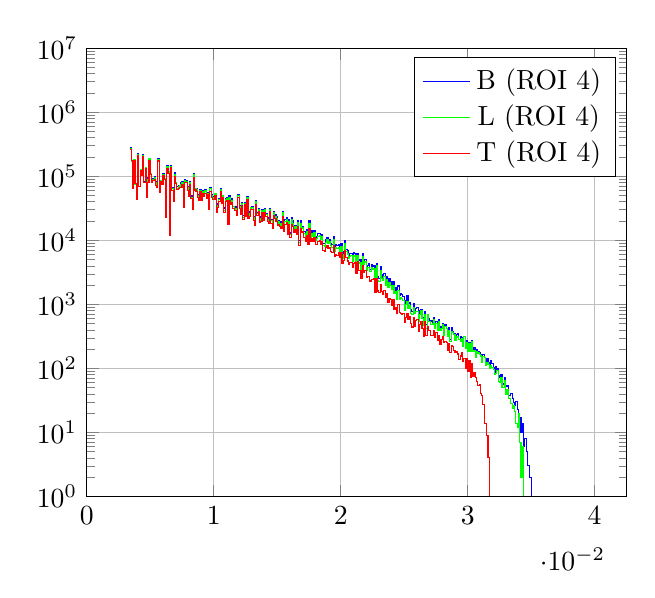
\begin{tikzpicture}

% Axis at [0.13 0.11 0.78 0.81]
\begin{semilogyaxis}[
xmajorgrids,
ymajorgrids,
xmin=0, xmax=0.0425,
ymin=1, ymax=1e+007,
%title={ROI 4},
legend entries={%
	B (ROI 4),%
	L (ROI 4),%
	T (ROI 4)}
]

\addplot [
color=blue,
solid
]coordinates{
 (0.0034,0) (0.0034,281790) (0.0034,281790) (0.0035,281790) (0.0035,168687) (0.0035,168687) (0.0036,168687) (0.0036,64147) (0.0036,64147) (0.0037,64147) (0.0037,183472) (0.0037,183472) (0.0038,183472) (0.0038,74451) (0.0038,74451) (0.0039,74451) (0.0039,51365) (0.0039,51365) (0.004,51365) (0.004,224801) (0.004,224801) (0.0041,224801) (0.0041,70097) (0.0041,70097) (0.0042,70097) (0.0042,125212) (0.0042,125212) (0.0043,125212) (0.0043,109648) (0.0043,109648) (0.0044,109648) (0.0044,217207) (0.0044,217207) (0.0045,217207) (0.0045,81721) (0.0045,81721) (0.0046,81721) (0.0046,138624) (0.0046,138624) (0.0047,138624) (0.0047,46672) (0.0047,46672) (0.0048,46672) (0.0048,94805) (0.0048,94805) (0.0049,94805) (0.0049,187740) (0.0049,187740) (0.005,187740) (0.005,109370) (0.005,109370) (0.0051,109370) (0.0051,82301) (0.0051,82301) (0.0052,82301) (0.0052,92493) (0.0052,92493) (0.0053,92493) (0.0053,97228) (0.0053,97228) (0.0054,97228) (0.0054,83152) (0.0054,83152) (0.0055,83152) (0.0055,68662) (0.0055,68662) (0.0056,68662) (0.0056,188624) (0.0056,188624) (0.0057,188624) (0.0057,60984) (0.0057,60984) (0.0058,60984) (0.0058,85874) (0.0058,85874) (0.0059,85874) (0.0059,86027) (0.0059,86027) (0.006,86027) (0.006,109570) (0.006,109570) (0.0061,109570) (0.0061,93178) (0.0061,93178) (0.0062,93178) (0.0062,28103) (0.0062,28103) (0.0063,28103) (0.0063,147873) (0.0063,147873) (0.0064,147873) (0.0064,119602) (0.0064,119602) (0.0065,119602) (0.0065,13881) (0.0065,13881) (0.0066,13881) (0.0066,147520) (0.0066,147520) (0.0067,147520) (0.0067,66635) (0.0067,66635) (0.0068,66635) (0.0068,50370) (0.0068,50370) (0.0069,50370) (0.0069,113021) (0.0069,113021) (0.007,113021) (0.007,79064) (0.007,79064) (0.0071,79064) (0.0071,68305) (0.0071,68305) (0.0072,68305) (0.0072,70929) (0.0072,70929) (0.0073,70929) (0.0073,72124) (0.0073,72124) (0.0074,72124) (0.0074,78397) (0.0074,78397) (0.0075,78397) (0.0075,82065) (0.0075,82065) (0.0076,82065) (0.0076,34686) (0.0076,34686) (0.0077,34686) (0.0077,88966) (0.0077,88966) (0.0078,88966) (0.0078,86468) (0.0078,86468) (0.0079,86468) (0.0079,68796) (0.0079,68796) (0.008,68796) (0.008,53451) (0.008,53451) (0.0081,53451) (0.0081,83440) (0.0081,83440) (0.0082,83440) (0.0082,49125) (0.0082,49125) (0.0083,49125) (0.0083,32723) (0.0083,32723) (0.0084,32723) (0.0084,110465) (0.0084,110465) (0.0085,110465) (0.0085,64697) (0.0085,64697) (0.0086,64697) (0.0086,63310) (0.0086,63310) (0.0087,63310) (0.0087,52216) (0.0087,52216) (0.0088,52216) (0.0088,48434) (0.0088,48434) (0.0089,48434) (0.0089,63050) (0.0089,63050) (0.009,63050) (0.009,46325) (0.009,46325) (0.0091,46325) (0.0091,58974) (0.0091,58974) (0.0092,58974) (0.0092,51474) (0.0092,51474) (0.0093,51474) (0.0093,61839) (0.0093,61839) (0.0094,61839) (0.0094,49505) (0.0094,49505) (0.0095,49505) (0.0095,55442) (0.0095,55442) (0.0096,55442) (0.0096,33007) (0.0096,33007) (0.0097,33007) (0.0097,67081) (0.0097,67081) (0.0098,67081) (0.0098,52082) (0.0098,52082) (0.0099,52082) (0.0099,46933) (0.0099,46933) (0.01,46933) (0.01,47979) (0.01,47979) (0.0101,47979) (0.0101,54391) (0.0101,54391) (0.0102,54391) (0.0102,30963) (0.0102,30963) (0.0103,30963) (0.0103,37071) (0.0103,37071) (0.0104,37071) (0.0104,45197) (0.0104,45197) (0.0105,45197) (0.0105,64518) (0.0105,64518) (0.0106,64518) (0.0106,41823) (0.0106,41823) (0.0107,41823) (0.0107,50716) (0.0107,50716) (0.0108,50716) (0.0108,31938) (0.0108,31938) (0.0109,31938) (0.0109,45127) (0.0109,45127) (0.011,45127) (0.011,46570) (0.011,46570) (0.0111,46570) (0.0111,20126) (0.0111,20126) (0.0112,20126) (0.0112,49088) (0.0112,49088) (0.0113,49088) (0.0113,41188) (0.0113,41188) (0.0114,41188) (0.0114,44329) (0.0114,44329) (0.0115,44329) (0.0115,34083) (0.0115,34083) (0.0116,34083) (0.0116,32041) (0.0116,32041) (0.0117,32041) (0.0117,33471) (0.0117,33471) (0.0118,33471) (0.0118,27855) (0.0118,27855) (0.0119,27855) (0.0119,52516) (0.0119,52516) (0.012,52516) (0.012,34779) (0.012,34779) (0.0121,34779) (0.0121,27427) (0.0121,27427) (0.0122,27427) (0.0122,38907) (0.0122,38907) (0.0123,38907) (0.0123,24409) (0.0123,24409) (0.0124,24409) (0.0124,39216) (0.0124,39216) (0.0125,39216) (0.0125,27562) (0.0125,27562) (0.0126,27562) (0.0126,47965) (0.0126,47965) (0.0127,47965) (0.0127,24612) (0.0127,24612) (0.0128,24612) (0.0128,28161) (0.0128,28161) (0.0129,28161) (0.0129,32843) (0.0129,32843) (0.013,32843) (0.013,33974) (0.013,33974) (0.0131,33974) (0.0131,23639) (0.0131,23639) (0.0132,23639) (0.0132,19381) (0.0132,19381) (0.0133,19381) (0.0133,41832) (0.0133,41832) (0.0134,41832) (0.0134,27262) (0.0134,27262) (0.0135,27262) (0.0135,31270) (0.0135,31270) (0.0136,31270) (0.0136,21165) (0.0136,21165) (0.0137,21165) (0.0137,23576) (0.0137,23576) (0.0138,23576) (0.0138,30490) (0.0138,30490) (0.0139,30490) (0.0139,23321) (0.0139,23321) (0.014,23321) (0.014,31710) (0.014,31710) (0.0141,31710) (0.0141,26187) (0.0141,26187) (0.0142,26187) (0.0142,22554) (0.0142,22554) (0.0143,22554) (0.0143,20740) (0.0143,20740) (0.0144,20740) (0.0144,31666) (0.0144,31666) (0.0145,31666) (0.0145,21389) (0.0145,21389) (0.0146,21389) (0.0146,17944) (0.0146,17944) (0.0147,17944) (0.0147,28503) (0.0147,28503) (0.0148,28503) (0.0148,25147) (0.0148,25147) (0.0149,25147) (0.0149,23160) (0.0149,23160) (0.015,23160) (0.015,19073) (0.015,19073) (0.0151,19073) (0.0151,20413) (0.0151,20413) (0.0152,20413) (0.0152,19280) (0.0152,19280) (0.0153,19280) (0.0153,18483) (0.0153,18483) (0.0154,18483) (0.0154,28334) (0.0154,28334) (0.0155,28334) (0.0155,15680) (0.0155,15680) (0.0156,15680) (0.0156,21249) (0.0156,21249) (0.0157,21249) (0.0157,22746) (0.0157,22746) (0.0158,22746) (0.0158,14662) (0.0158,14662) (0.0159,14662) (0.0159,21386) (0.0159,21386) (0.016,21386) (0.016,13020) (0.016,13020) (0.0161,13020) (0.0161,22399) (0.0161,22399) (0.0162,22399) (0.0162,20017) (0.0162,20017) (0.0163,20017) (0.0163,16458) (0.0163,16458) (0.0164,16458) (0.0164,17252) (0.0164,17252) (0.0165,17252) (0.0165,15524) (0.0165,15524) (0.0166,15524) (0.0166,20194) (0.0166,20194) (0.0167,20194) (0.0167,9839) (0.0167,9839) (0.0168,9839) (0.0168,20232) (0.0168,20232) (0.0169,20232) (0.0169,16104) (0.0169,16104) (0.017,16104) (0.017,16666) (0.017,16666) (0.0171,16666) (0.0171,13762) (0.0171,13762) (0.0172,13762) (0.0172,12442) (0.0172,12442) (0.0173,12442) (0.0173,14897) (0.0173,14897) (0.0174,14897) (0.0174,10641) (0.0174,10641) (0.0175,10641) (0.0175,20155) (0.0175,20155) (0.0176,20155) (0.0176,11833) (0.0176,11833) (0.0177,11833) (0.0177,14078) (0.0177,14078) (0.0178,14078) (0.0178,12455) (0.0178,12455) (0.0179,12455) (0.0179,14163) (0.0179,14163) (0.018,14163) (0.018,10944) (0.018,10944) (0.0181,10944) (0.0181,11617) (0.0181,11617) (0.0182,11617) (0.0182,12567) (0.0182,12567) (0.0183,12567) (0.0183,12826) (0.0183,12826) (0.0184,12826) (0.0184,11283) (0.0184,11283) (0.0185,11283) (0.0185,12297) (0.0185,12297) (0.0186,12297) (0.0186,8971) (0.0186,8971) (0.0187,8971) (0.0187,8952) (0.0187,8952) (0.0188,8952) (0.0188,10246) (0.0188,10246) (0.0189,10246) (0.0189,11137) (0.0189,11137) (0.019,11137) (0.019,9710) (0.019,9710) (0.0191,9710) (0.0191,10331) (0.0191,10331) (0.0192,10331) (0.0192,8949) (0.0192,8949) (0.0193,8949) (0.0193,8504) (0.0193,8504) (0.0194,8504) (0.0194,11245) (0.0194,11245) (0.0195,11245) (0.0195,7406) (0.0195,7406) (0.0196,7406) (0.0196,8475) (0.0196,8475) (0.0197,8475) (0.0197,8179) (0.0197,8179) (0.0198,8179) (0.0198,8496) (0.0198,8496) (0.0199,8496) (0.0199,7178) (0.0199,7178) (0.02,7178) (0.02,8824) (0.02,8824) (0.0201,8824) (0.0201,5735) (0.0201,5735) (0.0202,5735) (0.0202,6746) (0.0202,6746) (0.0203,6746) (0.0203,9878) (0.0203,9878) (0.0204,9878) (0.0204,7175) (0.0204,7175) (0.0205,7175) (0.0205,6824) (0.0205,6824) (0.0206,6824) (0.0206,5743) (0.0206,5743) (0.0207,5743) (0.0207,6270) (0.0207,6270) (0.0208,6270) (0.0208,6239) (0.0208,6239) (0.0209,6239) (0.0209,5107) (0.0209,5107) (0.021,5107) (0.021,6425) (0.021,6425) (0.0211,6425) (0.0211,6234) (0.0211,6234) (0.0212,6234) (0.0212,4529) (0.0212,4529) (0.0213,4529) (0.0213,6309) (0.0213,6309) (0.0214,6309) (0.0214,4819) (0.0214,4819) (0.0215,4819) (0.0215,4919) (0.0215,4919) (0.0216,4919) (0.0216,3530) (0.0216,3530) (0.0217,3530) (0.0217,6248) (0.0217,6248) (0.0218,6248) (0.0218,4633) (0.0218,4633) (0.0219,4633) (0.0219,5022) (0.0219,5022) (0.022,5022) (0.022,3834) (0.022,3834) (0.0221,3834) (0.0221,4067) (0.0221,4067) (0.0222,4067) (0.0222,4313) (0.0222,4313) (0.0223,4313) (0.0223,3554) (0.0223,3554) (0.0224,3554) (0.0224,4208) (0.0224,4208) (0.0225,4208) (0.0225,3888) (0.0225,3888) (0.0226,3888) (0.0226,3964) (0.0226,3964) (0.0227,3964) (0.0227,2656) (0.0227,2656) (0.0228,2656) (0.0228,4399) (0.0228,4399) (0.0229,4399) (0.0229,2691) (0.0229,2691) (0.023,2691) (0.023,2559) (0.023,2559) (0.0231,2559) (0.0231,3889) (0.0231,3889) (0.0232,3889) (0.0232,2942) (0.0232,2942) (0.0233,2942) (0.0233,2648) (0.0233,2648) (0.0234,2648) (0.0234,3073) (0.0234,3073) (0.0235,3073) (0.0235,2284) (0.0235,2284) (0.0236,2284) (0.0236,2758) (0.0236,2758) (0.0237,2758) (0.0237,2133) (0.0237,2133) (0.0238,2133) (0.0238,2532) (0.0238,2532) (0.0239,2532) (0.0239,2306) (0.0239,2306) (0.024,2306) (0.024,1965) (0.024,1965) (0.0241,1965) (0.0241,2298) (0.0241,2298) (0.0242,2298) (0.0242,1673) (0.0242,1673) (0.0243,1673) (0.0243,1843) (0.0243,1843) (0.0244,1843) (0.0244,1467) (0.0244,1467) (0.0245,1467) (0.0245,1935) (0.0245,1935) (0.0246,1935) (0.0246,1377) (0.0246,1377) (0.0247,1377) (0.0247,1459) (0.0247,1459) (0.0248,1459) (0.0248,1423) (0.0248,1423) (0.0249,1423) (0.0249,1346) (0.0249,1346) (0.025,1346) (0.025,947) (0.025,947) (0.0251,947) (0.0251,1162) (0.0251,1162) (0.0252,1162) (0.0252,1351) (0.0252,1351) (0.0253,1351) (0.0253,1019) (0.0253,1019) (0.0254,1019) (0.0254,1058) (0.0254,1058) (0.0255,1058) (0.0255,832) (0.0255,832) (0.0256,832) (0.0256,783) (0.0256,783) (0.0257,783) (0.0257,1018) (0.0257,1018) (0.0258,1018) (0.0258,801) (0.0258,801) (0.0259,801) (0.0259,867) (0.0259,867) (0.026,867) (0.026,887) (0.026,887) (0.0261,887) (0.0261,571) (0.0261,571) (0.0262,571) (0.0262,803) (0.0262,803) (0.0263,803) (0.0263,825) (0.0263,825) (0.0264,825) (0.0264,631) (0.0264,631) (0.0265,631) (0.0265,527) (0.0265,527) (0.0266,527) (0.0266,759) (0.0266,759) (0.0267,759) (0.0267,488) (0.0267,488) (0.0268,488) (0.0268,686) (0.0268,686) (0.0269,686) (0.0269,590) (0.0269,590) (0.027,590) (0.027,568) (0.027,568) (0.0271,568) (0.0271,549) (0.0271,549) (0.0272,549) (0.0272,506) (0.0272,506) (0.0273,506) (0.0273,619) (0.0273,619) (0.0274,619) (0.0274,432) (0.0274,432) (0.0275,432) (0.0275,543) (0.0275,543) (0.0276,543) (0.0276,411) (0.0276,411) (0.0277,411) (0.0277,575) (0.0277,575) (0.0278,575) (0.0278,413) (0.0278,413) (0.0279,413) (0.0279,451) (0.0279,451) (0.028,451) (0.028,508) (0.028,508) (0.0281,508) (0.0281,370) (0.0281,370) (0.0282,370) (0.0282,475) (0.0282,475) (0.0283,475) (0.0283,423) (0.0283,423) (0.0284,423) (0.0284,338) (0.0284,338) (0.0285,338) (0.0285,434) (0.0285,434) (0.0286,434) (0.0286,283) (0.0286,283) (0.0287,283) (0.0287,433) (0.0287,433) (0.0288,433) (0.0288,375) (0.0288,375) (0.0289,375) (0.0289,347) (0.0289,347) (0.029,347) (0.029,288) (0.029,288) (0.0291,288) (0.0291,337) (0.0291,337) (0.0292,337) (0.0292,344) (0.0292,344) (0.0293,344) (0.0293,280) (0.0293,280) (0.0294,280) (0.0294,317) (0.0294,317) (0.0295,317) (0.0295,298) (0.0295,298) (0.0296,298) (0.0296,244) (0.0296,244) (0.0297,244) (0.0297,313) (0.0297,313) (0.0298,313) (0.0298,227) (0.0298,227) (0.0299,227) (0.0299,271) (0.0299,271) (0.03,271) (0.03,222) (0.03,222) (0.0301,222) (0.0301,253) (0.0301,253) (0.0302,253) (0.0302,208) (0.0302,208) (0.0303,208) (0.0303,274) (0.0303,274) (0.0304,274) (0.0304,186) (0.0304,186) (0.0305,186) (0.0305,212) (0.0305,212) (0.0306,212) (0.0306,174) (0.0306,174) (0.0307,174) (0.0307,197) (0.0307,197) (0.0308,197) (0.0308,180) (0.0308,180) (0.0309,180) (0.0309,175) (0.0309,175) (0.031,175) (0.031,164) (0.031,164) (0.0311,164) (0.0311,161) (0.0311,161) (0.0312,161) (0.0312,164) (0.0312,164) (0.0313,164) (0.0313,147) (0.0313,147) (0.0314,147) (0.0314,117) (0.0314,117) (0.0315,117) (0.0315,142) (0.0315,142) (0.0316,142) (0.0316,123) (0.0316,123) (0.0317,123) (0.0317,110) (0.0317,110) (0.0318,110) (0.0318,131) (0.0318,131) (0.0319,131) (0.0319,118) (0.0319,118) (0.032,118) (0.032,103) (0.032,103) (0.0321,103) (0.0321,82) (0.0321,82) (0.0322,82) (0.0322,106) (0.0322,106) (0.0323,106) (0.0323,98) (0.0323,98) (0.0324,98) (0.0324,76) (0.0324,76) (0.0325,76) (0.0325,72) (0.0325,72) (0.0326,72) (0.0326,79) (0.0326,79) (0.0327,79) (0.0327,57) (0.0327,57) (0.0328,57) (0.0328,56) (0.0328,56) (0.0329,56) (0.0329,72) (0.0329,72) (0.033,72) (0.033,52) (0.033,52) (0.0331,52) (0.0331,54) (0.0331,54) (0.0332,54) (0.0332,38) (0.0332,38) (0.0333,38) (0.0333,38) (0.0333,38) (0.0334,38) (0.0334,40) (0.0334,40) (0.0335,40) (0.0335,34) (0.0335,34) (0.0336,34) (0.0336,29) (0.0336,29) (0.0337,29) (0.0337,26) (0.0337,26) (0.0338,26) (0.0338,30) (0.0338,30) (0.0339,30) (0.0339,23) (0.0339,23) (0.034,23) (0.034,16) (0.034,16) (0.0341,16) (0.0341,17) (0.0341,17) (0.0342,17) (0.0342,10) (0.0342,10) (0.0343,10) (0.0343,14) (0.0343,14) (0.0344,14) (0.0344,6) (0.0344,6) (0.0345,6) (0.0345,8) (0.0345,8) (0.0346,8) (0.0346,5) (0.0346,5) (0.0347,5) (0.0347,3) (0.0347,3) (0.0348,3) (0.0348,3) (0.0348,3) (0.0349,3) (0.0349,2) (0.0349,2) (0.035,2) (0.035,1)
};

\addplot [
color=green,
solid
]coordinates{
 (0.0034,0) (0.0034,271598) (0.0034,271598) (0.0035,271598) (0.0035,172321) (0.0035,172321) (0.0036,172321) (0.0036,64685) (0.0036,64685) (0.0037,64685) (0.0037,179388) (0.0037,179388) (0.0038,179388) (0.0038,75745) (0.0038,75745) (0.0039,75745) (0.0039,48485) (0.0039,48485) (0.004,48485) (0.004,217792) (0.004,217792) (0.0041,217792) (0.0041,69854) (0.0041,69854) (0.0042,69854) (0.0042,125340) (0.0042,125340) (0.0043,125340) (0.0043,106837) (0.0043,106837) (0.0044,106837) (0.0044,211120) (0.0044,211120) (0.0045,211120) (0.0045,81090) (0.0045,81090) (0.0046,81090) (0.0046,134794) (0.0046,134794) (0.0047,134794) (0.0047,46636) (0.0047,46636) (0.0048,46636) (0.0048,87452) (0.0048,87452) (0.0049,87452) (0.0049,185602) (0.0049,185602) (0.005,185602) (0.005,108285) (0.005,108285) (0.0051,108285) (0.0051,80595) (0.0051,80595) (0.0052,80595) (0.0052,89130) (0.0052,89130) (0.0053,89130) (0.0053,93871) (0.0053,93871) (0.0054,93871) (0.0054,78797) (0.0054,78797) (0.0055,78797) (0.0055,68352) (0.0055,68352) (0.0056,68352) (0.0056,183152) (0.0056,183152) (0.0057,183152) (0.0057,59111) (0.0057,59111) (0.0058,59111) (0.0058,84509) (0.0058,84509) (0.0059,84509) (0.0059,81333) (0.0059,81333) (0.006,81333) (0.006,106593) (0.006,106593) (0.0061,106593) (0.0061,91206) (0.0061,91206) (0.0062,91206) (0.0062,26292) (0.0062,26292) (0.0063,26292) (0.0063,141663) (0.0063,141663) (0.0064,141663) (0.0064,117076) (0.0064,117076) (0.0065,117076) (0.0065,13013) (0.0065,13013) (0.0066,13013) (0.0066,143979) (0.0066,143979) (0.0067,143979) (0.0067,63455) (0.0067,63455) (0.0068,63455) (0.0068,46376) (0.0068,46376) (0.0069,46376) (0.0069,107528) (0.0069,107528) (0.007,107528) (0.007,78585) (0.007,78585) (0.0071,78585) (0.0071,65388) (0.0071,65388) (0.0072,65388) (0.0072,67906) (0.0072,67906) (0.0073,67906) (0.0073,70405) (0.0073,70405) (0.0074,70405) (0.0074,73895) (0.0074,73895) (0.0075,73895) (0.0075,79291) (0.0075,79291) (0.0076,79291) (0.0076,33761) (0.0076,33761) (0.0077,33761) (0.0077,84818) (0.0077,84818) (0.0078,84818) (0.0078,83367) (0.0078,83367) (0.0079,83367) (0.0079,65594) (0.0079,65594) (0.008,65594) (0.008,51344) (0.008,51344) (0.0081,51344) (0.0081,80645) (0.0081,80645) (0.0082,80645) (0.0082,47268) (0.0082,47268) (0.0083,47268) (0.0083,31366) (0.0083,31366) (0.0084,31366) (0.0084,104659) (0.0084,104659) (0.0085,104659) (0.0085,63417) (0.0085,63417) (0.0086,63417) (0.0086,61457) (0.0086,61457) (0.0087,61457) (0.0087,50171) (0.0087,50171) (0.0088,50171) (0.0088,45566) (0.0088,45566) (0.0089,45566) (0.0089,60555) (0.0089,60555) (0.009,60555) (0.009,44454) (0.009,44454) (0.0091,44454) (0.0091,57312) (0.0091,57312) (0.0092,57312) (0.0092,50260) (0.0092,50260) (0.0093,50260) (0.0093,58793) (0.0093,58793) (0.0094,58793) (0.0094,47298) (0.0094,47298) (0.0095,47298) (0.0095,54373) (0.0095,54373) (0.0096,54373) (0.0096,31927) (0.0096,31927) (0.0097,31927) (0.0097,63527) (0.0097,63527) (0.0098,63527) (0.0098,50304) (0.0098,50304) (0.0099,50304) (0.0099,45391) (0.0099,45391) (0.01,45391) (0.01,46241) (0.01,46241) (0.0101,46241) (0.0101,52768) (0.0101,52768) (0.0102,52768) (0.0102,29422) (0.0102,29422) (0.0103,29422) (0.0103,35054) (0.0103,35054) (0.0104,35054) (0.0104,43319) (0.0104,43319) (0.0105,43319) (0.0105,61777) (0.0105,61777) (0.0106,61777) (0.0106,40538) (0.0106,40538) (0.0107,40538) (0.0107,49448) (0.0107,49448) (0.0108,49448) (0.0108,29661) (0.0108,29661) (0.0109,29661) (0.0109,43735) (0.0109,43735) (0.011,43735) (0.011,44987) (0.011,44987) (0.0111,44987) (0.0111,19068) (0.0111,19068) (0.0112,19068) (0.0112,46720) (0.0112,46720) (0.0113,46720) (0.0113,39601) (0.0113,39601) (0.0114,39601) (0.0114,42456) (0.0114,42456) (0.0115,42456) (0.0115,33219) (0.0115,33219) (0.0116,33219) (0.0116,30804) (0.0116,30804) (0.0117,30804) (0.0117,31753) (0.0117,31753) (0.0118,31753) (0.0118,26259) (0.0118,26259) (0.0119,26259) (0.0119,50388) (0.0119,50388) (0.012,50388) (0.012,33765) (0.012,33765) (0.0121,33765) (0.0121,26360) (0.0121,26360) (0.0122,26360) (0.0122,37251) (0.0122,37251) (0.0123,37251) (0.0123,22864) (0.0123,22864) (0.0124,22864) (0.0124,38087) (0.0124,38087) (0.0125,38087) (0.0125,25879) (0.0125,25879) (0.0126,25879) (0.0126,46307) (0.0126,46307) (0.0127,46307) (0.0127,23698) (0.0127,23698) (0.0128,23698) (0.0128,26526) (0.0128,26526) (0.0129,26526) (0.0129,31901) (0.0129,31901) (0.013,31901) (0.013,32519) (0.013,32519) (0.0131,32519) (0.0131,22345) (0.0131,22345) (0.0132,22345) (0.0132,18597) (0.0132,18597) (0.0133,18597) (0.0133,39876) (0.0133,39876) (0.0134,39876) (0.0134,25938) (0.0134,25938) (0.0135,25938) (0.0135,30158) (0.0135,30158) (0.0136,30158) (0.0136,20354) (0.0136,20354) (0.0137,20354) (0.0137,22184) (0.0137,22184) (0.0138,22184) (0.0138,28964) (0.0138,28964) (0.0139,28964) (0.0139,22057) (0.0139,22057) (0.014,22057) (0.014,30233) (0.014,30233) (0.0141,30233) (0.0141,25127) (0.0141,25127) (0.0142,25127) (0.0142,21408) (0.0142,21408) (0.0143,21408) (0.0143,19627) (0.0143,19627) (0.0144,19627) (0.0144,30202) (0.0144,30202) (0.0145,30202) (0.0145,20136) (0.0145,20136) (0.0146,20136) (0.0146,16800) (0.0146,16800) (0.0147,16800) (0.0147,26933) (0.0147,26933) (0.0148,26933) (0.0148,23822) (0.0148,23822) (0.0149,23822) (0.0149,21923) (0.0149,21923) (0.015,21923) (0.015,18236) (0.015,18236) (0.0151,18236) (0.0151,19299) (0.0151,19299) (0.0152,19299) (0.0152,18011) (0.0152,18011) (0.0153,18011) (0.0153,17154) (0.0153,17154) (0.0154,17154) (0.0154,26735) (0.0154,26735) (0.0155,26735) (0.0155,14903) (0.0155,14903) (0.0156,14903) (0.0156,19867) (0.0156,19867) (0.0157,19867) (0.0157,21405) (0.0157,21405) (0.0158,21405) (0.0158,13716) (0.0158,13716) (0.0159,13716) (0.0159,19819) (0.0159,19819) (0.016,19819) (0.016,12277) (0.016,12277) (0.0161,12277) (0.0161,20789) (0.0161,20789) (0.0162,20789) (0.0162,18563) (0.0162,18563) (0.0163,18563) (0.0163,15371) (0.0163,15371) (0.0164,15371) (0.0164,16192) (0.0164,16192) (0.0165,16192) (0.0165,14460) (0.0165,14460) (0.0166,14460) (0.0166,18838) (0.0166,18838) (0.0167,18838) (0.0167,9349) (0.0167,9349) (0.0168,9349) (0.0168,18416) (0.0168,18416) (0.0169,18416) (0.0169,15104) (0.0169,15104) (0.017,15104) (0.017,15620) (0.017,15620) (0.0171,15620) (0.0171,12651) (0.0171,12651) (0.0172,12651) (0.0172,11357) (0.0172,11357) (0.0173,11357) (0.0173,13827) (0.0173,13827) (0.0174,13827) (0.0174,9864) (0.0174,9864) (0.0175,9864) (0.0175,18316) (0.0175,18316) (0.0176,18316) (0.0176,11046) (0.0176,11046) (0.0177,11046) (0.0177,12974) (0.0177,12974) (0.0178,12974) (0.0178,11409) (0.0178,11409) (0.0179,11409) (0.0179,13029) (0.0179,13029) (0.018,13029) (0.018,10006) (0.018,10006) (0.0181,10006) (0.0181,10551) (0.0181,10551) (0.0182,10551) (0.0182,11614) (0.0182,11614) (0.0183,11614) (0.0183,11684) (0.0183,11684) (0.0184,11684) (0.0184,10377) (0.0184,10377) (0.0185,10377) (0.0185,11342) (0.0185,11342) (0.0186,11342) (0.0186,8325) (0.0186,8325) (0.0187,8325) (0.0187,8153) (0.0187,8153) (0.0188,8153) (0.0188,9281) (0.0188,9281) (0.0189,9281) (0.0189,10287) (0.0189,10287) (0.019,10287) (0.019,9052) (0.019,9052) (0.0191,9052) (0.0191,9436) (0.0191,9436) (0.0192,9436) (0.0192,8165) (0.0192,8165) (0.0193,8165) (0.0193,7714) (0.0193,7714) (0.0194,7714) (0.0194,10363) (0.0194,10363) (0.0195,10363) (0.0195,6733) (0.0195,6733) (0.0196,6733) (0.0196,7744) (0.0196,7744) (0.0197,7744) (0.0197,7366) (0.0197,7366) (0.0198,7366) (0.0198,7824) (0.0198,7824) (0.0199,7824) (0.0199,6639) (0.0199,6639) (0.02,6639) (0.02,7922) (0.02,7922) (0.0201,7922) (0.0201,5288) (0.0201,5288) (0.0202,5288) (0.0202,6066) (0.0202,6066) (0.0203,6066) (0.0203,8871) (0.0203,8871) (0.0204,8871) (0.0204,6669) (0.0204,6669) (0.0205,6669) (0.0205,6103) (0.0205,6103) (0.0206,6103) (0.0206,5292) (0.0206,5292) (0.0207,5292) (0.0207,5580) (0.0207,5580) (0.0208,5580) (0.0208,5713) (0.0208,5713) (0.0209,5713) (0.0209,4593) (0.0209,4593) (0.021,4593) (0.021,5820) (0.021,5820) (0.0211,5820) (0.0211,5687) (0.0211,5687) (0.0212,5687) (0.0212,4029) (0.0212,4029) (0.0213,4029) (0.0213,5764) (0.0213,5764) (0.0214,5764) (0.0214,4410) (0.0214,4410) (0.0215,4410) (0.0215,4435) (0.0215,4435) (0.0216,4435) (0.0216,3203) (0.0216,3203) (0.0217,3203) (0.0217,5529) (0.0217,5529) (0.0218,5529) (0.0218,4174) (0.0218,4174) (0.0219,4174) (0.0219,4591) (0.0219,4591) (0.022,4591) (0.022,3386) (0.022,3386) (0.0221,3386) (0.0221,3728) (0.0221,3728) (0.0222,3728) (0.0222,3796) (0.0222,3796) (0.0223,3796) (0.0223,3242) (0.0223,3242) (0.0224,3242) (0.0224,3713) (0.0224,3713) (0.0225,3713) (0.0225,3507) (0.0225,3507) (0.0226,3507) (0.0226,3565) (0.0226,3565) (0.0227,3565) (0.0227,2296) (0.0227,2296) (0.0228,2296) (0.0228,3967) (0.0228,3967) (0.0229,3967) (0.0229,2394) (0.0229,2394) (0.023,2394) (0.023,2269) (0.023,2269) (0.0231,2269) (0.0231,3410) (0.0231,3410) (0.0232,3410) (0.0232,2520) (0.0232,2520) (0.0233,2520) (0.0233,2320) (0.0233,2320) (0.0234,2320) (0.0234,2752) (0.0234,2752) (0.0235,2752) (0.0235,1999) (0.0235,1999) (0.0236,1999) (0.0236,2428) (0.0236,2428) (0.0237,2428) (0.0237,1857) (0.0237,1857) (0.0238,1857) (0.0238,2150) (0.0238,2150) (0.0239,2150) (0.0239,1998) (0.0239,1998) (0.024,1998) (0.024,1685) (0.024,1685) (0.0241,1685) (0.0241,1984) (0.0241,1984) (0.0242,1984) (0.0242,1465) (0.0242,1465) (0.0243,1465) (0.0243,1588) (0.0243,1588) (0.0244,1588) (0.0244,1210) (0.0244,1210) (0.0245,1210) (0.0245,1650) (0.0245,1650) (0.0246,1650) (0.0246,1174) (0.0246,1174) (0.0247,1174) (0.0247,1257) (0.0247,1257) (0.0248,1257) (0.0248,1216) (0.0248,1216) (0.0249,1216) (0.0249,1146) (0.0249,1146) (0.025,1146) (0.025,803) (0.025,803) (0.0251,803) (0.0251,989) (0.0251,989) (0.0252,989) (0.0252,1110) (0.0252,1110) (0.0253,1110) (0.0253,849) (0.0253,849) (0.0254,849) (0.0254,973) (0.0254,973) (0.0255,973) (0.0255,713) (0.0255,713) (0.0256,713) (0.0256,686) (0.0256,686) (0.0257,686) (0.0257,881) (0.0257,881) (0.0258,881) (0.0258,714) (0.0258,714) (0.0259,714) (0.0259,766) (0.0259,766) (0.026,766) (0.026,769) (0.026,769) (0.0261,769) (0.0261,541) (0.0261,541) (0.0262,541) (0.0262,699) (0.0262,699) (0.0263,699) (0.0263,796) (0.0263,796) (0.0264,796) (0.0264,603) (0.0264,603) (0.0265,603) (0.0265,464) (0.0265,464) (0.0266,464) (0.0266,691) (0.0266,691) (0.0267,691) (0.0267,425) (0.0267,425) (0.0268,425) (0.0268,689) (0.0268,689) (0.0269,689) (0.0269,546) (0.0269,546) (0.027,546) (0.027,548) (0.027,548) (0.0271,548) (0.0271,485) (0.0271,485) (0.0272,485) (0.0272,494) (0.0272,494) (0.0273,494) (0.0273,576) (0.0273,576) (0.0274,576) (0.0274,426) (0.0274,426) (0.0275,426) (0.0275,507) (0.0275,507) (0.0276,507) (0.0276,397) (0.0276,397) (0.0277,397) (0.0277,537) (0.0277,537) (0.0278,537) (0.0278,396) (0.0278,396) (0.0279,396) (0.0279,420) (0.0279,420) (0.028,420) (0.028,478) (0.028,478) (0.0281,478) (0.0281,324) (0.0281,324) (0.0282,324) (0.0282,450) (0.0282,450) (0.0283,450) (0.0283,423) (0.0283,423) (0.0284,423) (0.0284,317) (0.0284,317) (0.0285,317) (0.0285,396) (0.0285,396) (0.0286,396) (0.0286,264) (0.0286,264) (0.0287,264) (0.0287,381) (0.0287,381) (0.0288,381) (0.0288,364) (0.0288,364) (0.0289,364) (0.0289,341) (0.0289,341) (0.029,341) (0.029,271) (0.029,271) (0.0291,271) (0.0291,311) (0.0291,311) (0.0292,311) (0.0292,309) (0.0292,309) (0.0293,309) (0.0293,279) (0.0293,279) (0.0294,279) (0.0294,264) (0.0294,264) (0.0295,264) (0.0295,292) (0.0295,292) (0.0296,292) (0.0296,217) (0.0296,217) (0.0297,217) (0.0297,315) (0.0297,315) (0.0298,315) (0.0298,208) (0.0298,208) (0.0299,208) (0.0299,257) (0.0299,257) (0.03,257) (0.03,184) (0.03,184) (0.0301,184) (0.0301,244) (0.0301,244) (0.0302,244) (0.0302,185) (0.0302,185) (0.0303,185) (0.0303,260) (0.0303,260) (0.0304,260) (0.0304,183) (0.0304,183) (0.0305,183) (0.0305,191) (0.0305,191) (0.0306,191) (0.0306,147) (0.0306,147) (0.0307,147) (0.0307,181) (0.0307,181) (0.0308,181) (0.0308,174) (0.0308,174) (0.0309,174) (0.0309,166) (0.0309,166) (0.031,166) (0.031,156) (0.031,156) (0.0311,156) (0.0311,122) (0.0311,122) (0.0312,122) (0.0312,152) (0.0312,152) (0.0313,152) (0.0313,146) (0.0313,146) (0.0314,146) (0.0314,110) (0.0314,110) (0.0315,110) (0.0315,124) (0.0315,124) (0.0316,124) (0.0316,115) (0.0316,115) (0.0317,115) (0.0317,99) (0.0317,99) (0.0318,99) (0.0318,111) (0.0318,111) (0.0319,111) (0.0319,104) (0.0319,104) (0.032,104) (0.032,95) (0.032,95) (0.0321,95) (0.0321,80) (0.0321,80) (0.0322,80) (0.0322,83) (0.0322,83) (0.0323,83) (0.0323,92) (0.0323,92) (0.0324,92) (0.0324,63) (0.0324,63) (0.0325,63) (0.0325,61) (0.0325,61) (0.0326,61) (0.0326,72) (0.0326,72) (0.0327,72) (0.0327,51) (0.0327,51) (0.0328,51) (0.0328,50) (0.0328,50) (0.0329,50) (0.0329,64) (0.0329,64) (0.033,64) (0.033,39) (0.033,39) (0.0331,39) (0.0331,46) (0.0331,46) (0.0332,46) (0.0332,34) (0.0332,34) (0.0333,34) (0.0333,34) (0.0333,34) (0.0334,34) (0.0334,28) (0.0334,28) (0.0335,28) (0.0335,24) (0.0335,24) (0.0336,24) (0.0336,26) (0.0336,26) (0.0337,26) (0.0337,21) (0.0337,21) (0.0338,21) (0.0338,14) (0.0338,14) (0.0339,14) (0.0339,12) (0.0339,12) (0.034,12) (0.034,20) (0.034,20) (0.0341,20) (0.0341,7) (0.0341,7) (0.0342,7) (0.0342,2) (0.0342,2) (0.0343,2) (0.0343,6) (0.0343,6) (0.0344,6) (0.0344,1)
};

\addplot [
color=red,
solid
]coordinates{
 (0.0034,0) (0.0034,257512) (0.0034,257512) (0.0035,257512) (0.0035,175936) (0.0035,175936) (0.0036,175936) (0.0036,64707) (0.0036,64707) (0.0037,64707) (0.0037,174999) (0.0037,174999) (0.0038,174999) (0.0038,77453) (0.0038,77453) (0.0039,77453) (0.0039,43250) (0.0039,43250) (0.004,43250) (0.004,208640) (0.004,208640) (0.0041,208640) (0.0041,70071) (0.0041,70071) (0.0042,70071) (0.0042,123520) (0.0042,123520) (0.0043,123520) (0.0043,104650) (0.0043,104650) (0.0044,104650) (0.0044,200969) (0.0044,200969) (0.0045,200969) (0.0045,80123) (0.0045,80123) (0.0046,80123) (0.0046,129656) (0.0046,129656) (0.0047,129656) (0.0047,46922) (0.0047,46922) (0.0048,46922) (0.0048,80160) (0.0048,80160) (0.0049,80160) (0.0049,178102) (0.0049,178102) (0.005,178102) (0.005,105383) (0.005,105383) (0.0051,105383) (0.0051,78942) (0.0051,78942) (0.0052,78942) (0.0052,84976) (0.0052,84976) (0.0053,84976) (0.0053,88634) (0.0053,88634) (0.0054,88634) (0.0054,72584) (0.0054,72584) (0.0055,72584) (0.0055,67808) (0.0055,67808) (0.0056,67808) (0.0056,172941) (0.0056,172941) (0.0057,172941) (0.0057,56236) (0.0057,56236) (0.0058,56236) (0.0058,82668) (0.0058,82668) (0.0059,82668) (0.0059,73316) (0.0059,73316) (0.006,73316) (0.006,102809) (0.006,102809) (0.0061,102809) (0.0061,88049) (0.0061,88049) (0.0062,88049) (0.0062,23100) (0.0062,23100) (0.0063,23100) (0.0063,133691) (0.0063,133691) (0.0064,133691) (0.0064,110880) (0.0064,110880) (0.0065,110880) (0.0065,11699) (0.0065,11699) (0.0066,11699) (0.0066,138069) (0.0066,138069) (0.0067,138069) (0.0067,59712) (0.0067,59712) (0.0068,59712) (0.0068,41068) (0.0068,41068) (0.0069,41068) (0.0069,99785) (0.0069,99785) (0.007,99785) (0.007,76300) (0.007,76300) (0.0071,76300) (0.0071,61808) (0.0071,61808) (0.0072,61808) (0.0072,63466) (0.0072,63466) (0.0073,63466) (0.0073,67204) (0.0073,67204) (0.0074,67204) (0.0074,67560) (0.0074,67560) (0.0075,67560) (0.0075,74727) (0.0075,74727) (0.0076,74727) (0.0076,32382) (0.0076,32382) (0.0077,32382) (0.0077,78728) (0.0077,78728) (0.0078,78728) (0.0078,78635) (0.0078,78635) (0.0079,78635) (0.0079,60280) (0.0079,60280) (0.008,60280) (0.008,48825) (0.008,48825) (0.0081,48825) (0.0081,75304) (0.0081,75304) (0.0082,75304) (0.0082,44920) (0.0082,44920) (0.0083,44920) (0.0083,29780) (0.0083,29780) (0.0084,29780) (0.0084,95358) (0.0084,95358) (0.0085,95358) (0.0085,60886) (0.0085,60886) (0.0086,60886) (0.0086,57853) (0.0086,57853) (0.0087,57853) (0.0087,47172) (0.0087,47172) (0.0088,47172) (0.0088,41409) (0.0088,41409) (0.0089,41409) (0.0089,56836) (0.0089,56836) (0.009,56836) (0.009,41330) (0.009,41330) (0.0091,41330) (0.0091,53077) (0.0091,53077) (0.0092,53077) (0.0092,48203) (0.0092,48203) (0.0093,48203) (0.0093,53776) (0.0093,53776) (0.0094,53776) (0.0094,44254) (0.0094,44254) (0.0095,44254) (0.0095,51518) (0.0095,51518) (0.0096,51518) (0.0096,30101) (0.0096,30101) (0.0097,30101) (0.0097,58681) (0.0097,58681) (0.0098,58681) (0.0098,46318) (0.0098,46318) (0.0099,46318) (0.0099,42753) (0.0099,42753) (0.01,42753) (0.01,43221) (0.01,43221) (0.0101,43221) (0.0101,49684) (0.0101,49684) (0.0102,49684) (0.0102,27346) (0.0102,27346) (0.0103,27346) (0.0103,32313) (0.0103,32313) (0.0104,32313) (0.0104,40301) (0.0104,40301) (0.0105,40301) (0.0105,57108) (0.0105,57108) (0.0106,57108) (0.0106,38153) (0.0106,38153) (0.0107,38153) (0.0107,46906) (0.0107,46906) (0.0108,46906) (0.0108,26860) (0.0108,26860) (0.0109,26860) (0.0109,40822) (0.0109,40822) (0.011,40822) (0.011,42438) (0.011,42438) (0.0111,42438) (0.0111,17934) (0.0111,17934) (0.0112,17934) (0.0112,42438) (0.0112,42438) (0.0113,42438) (0.0113,36831) (0.0113,36831) (0.0114,36831) (0.0114,39502) (0.0114,39502) (0.0115,39502) (0.0115,31420) (0.0115,31420) (0.0116,31420) (0.0116,28790) (0.0116,28790) (0.0117,28790) (0.0117,29421) (0.0117,29421) (0.0118,29421) (0.0118,24191) (0.0118,24191) (0.0119,24191) (0.0119,46052) (0.0119,46052) (0.012,46052) (0.012,31833) (0.012,31833) (0.0121,31833) (0.0121,24898) (0.0121,24898) (0.0122,24898) (0.0122,34593) (0.0122,34593) (0.0123,34593) (0.0123,20824) (0.0123,20824) (0.0124,20824) (0.0124,35883) (0.0124,35883) (0.0125,35883) (0.0125,23606) (0.0125,23606) (0.0126,23606) (0.0126,43044) (0.0126,43044) (0.0127,43044) (0.0127,22232) (0.0127,22232) (0.0128,22232) (0.0128,23634) (0.0128,23634) (0.0129,23634) (0.0129,30347) (0.0129,30347) (0.013,30347) (0.013,30300) (0.013,30300) (0.0131,30300) (0.0131,20632) (0.0131,20632) (0.0132,20632) (0.0132,17302) (0.0132,17302) (0.0133,17302) (0.0133,36249) (0.0133,36249) (0.0134,36249) (0.0134,24026) (0.0134,24026) (0.0135,24026) (0.0135,28236) (0.0135,28236) (0.0136,28236) (0.0136,19267) (0.0136,19267) (0.0137,19267) (0.0137,19825) (0.0137,19825) (0.0138,19825) (0.0138,26937) (0.0138,26937) (0.0139,26937) (0.0139,20150) (0.0139,20150) (0.014,20150) (0.014,27494) (0.014,27494) (0.0141,27494) (0.0141,23335) (0.0141,23335) (0.0142,23335) (0.0142,19784) (0.0142,19784) (0.0143,19784) (0.0143,18062) (0.0143,18062) (0.0144,18062) (0.0144,27792) (0.0144,27792) (0.0145,27792) (0.0145,18417) (0.0145,18417) (0.0146,18417) (0.0146,15169) (0.0146,15169) (0.0147,15169) (0.0147,24276) (0.0147,24276) (0.0148,24276) (0.0148,21703) (0.0148,21703) (0.0149,21703) (0.0149,19909) (0.0149,19909) (0.015,19909) (0.015,16758) (0.015,16758) (0.0151,16758) (0.0151,17548) (0.0151,17548) (0.0152,17548) (0.0152,16222) (0.0152,16222) (0.0153,16222) (0.0153,15129) (0.0153,15129) (0.0154,15129) (0.0154,23589) (0.0154,23589) (0.0155,23589) (0.0155,13705) (0.0155,13705) (0.0156,13705) (0.0156,17743) (0.0156,17743) (0.0157,17743) (0.0157,18862) (0.0157,18862) (0.0158,18862) (0.0158,12416) (0.0158,12416) (0.0159,12416) (0.0159,17599) (0.0159,17599) (0.016,17599) (0.016,11148) (0.016,11148) (0.0161,11148) (0.0161,17858) (0.0161,17858) (0.0162,17858) (0.0162,16229) (0.0162,16229) (0.0163,16229) (0.0163,13340) (0.0163,13340) (0.0164,13340) (0.0164,14713) (0.0164,14713) (0.0165,14713) (0.0165,12434) (0.0165,12434) (0.0166,12434) (0.0166,16406) (0.0166,16406) (0.0167,16406) (0.0167,8312) (0.0167,8312) (0.0168,8312) (0.0168,15420) (0.0168,15420) (0.0169,15420) (0.0169,13049) (0.0169,13049) (0.017,13049) (0.017,13467) (0.017,13467) (0.0171,13467) (0.0171,10894) (0.0171,10894) (0.0172,10894) (0.0172,9581) (0.0172,9581) (0.0173,9581) (0.0173,12018) (0.0173,12018) (0.0174,12018) (0.0174,8567) (0.0174,8567) (0.0175,8567) (0.0175,15169) (0.0175,15169) (0.0176,15169) (0.0176,9465) (0.0176,9465) (0.0177,9465) (0.0177,10818) (0.0177,10818) (0.0178,10818) (0.0178,9730) (0.0178,9730) (0.0179,9730) (0.0179,11160) (0.0179,11160) (0.018,11160) (0.018,8734) (0.018,8734) (0.0181,8734) (0.0181,8703) (0.0181,8703) (0.0182,8703) (0.0182,9478) (0.0182,9478) (0.0183,9478) (0.0183,9994) (0.0183,9994) (0.0184,9994) (0.0184,8676) (0.0184,8676) (0.0185,8676) (0.0185,9470) (0.0185,9470) (0.0186,9470) (0.0186,6946) (0.0186,6946) (0.0187,6946) (0.0187,6772) (0.0187,6772) (0.0188,6772) (0.0188,7751) (0.0188,7751) (0.0189,7751) (0.0189,8383) (0.0189,8383) (0.019,8383) (0.019,7439) (0.019,7439) (0.0191,7439) (0.0191,7615) (0.0191,7615) (0.0192,7615) (0.0192,6641) (0.0192,6641) (0.0193,6641) (0.0193,6386) (0.0193,6386) (0.0194,6386) (0.0194,8372) (0.0194,8372) (0.0195,8372) (0.0195,5693) (0.0195,5693) (0.0196,5693) (0.0196,6049) (0.0196,6049) (0.0197,6049) (0.0197,5836) (0.0197,5836) (0.0198,5836) (0.0198,6436) (0.0198,6436) (0.0199,6436) (0.0199,5355) (0.0199,5355) (0.02,5355) (0.02,6374) (0.02,6374) (0.0201,6374) (0.0201,4296) (0.0201,4296) (0.0202,4296) (0.0202,4897) (0.0202,4897) (0.0203,4897) (0.0203,6942) (0.0203,6942) (0.0204,6942) (0.0204,5451) (0.0204,5451) (0.0205,5451) (0.0205,4755) (0.0205,4755) (0.0206,4755) (0.0206,4153) (0.0206,4153) (0.0207,4153) (0.0207,4462) (0.0207,4462) (0.0208,4462) (0.0208,4533) (0.0208,4533) (0.0209,4533) (0.0209,3709) (0.0209,3709) (0.021,3709) (0.021,4338) (0.021,4338) (0.0211,4338) (0.0211,4448) (0.0211,4448) (0.0212,4448) (0.0212,2996) (0.0212,2996) (0.0213,2996) (0.0213,4579) (0.0213,4579) (0.0214,4579) (0.0214,3375) (0.0214,3375) (0.0215,3375) (0.0215,3383) (0.0215,3383) (0.0216,3383) (0.0216,2531) (0.0216,2531) (0.0217,2531) (0.0217,4040) (0.0217,4040) (0.0218,4040) (0.0218,3092) (0.0218,3092) (0.0219,3092) (0.0219,3364) (0.0219,3364) (0.022,3364) (0.022,2589) (0.022,2589) (0.0221,2589) (0.0221,2734) (0.0221,2734) (0.0222,2734) (0.0222,2724) (0.0222,2724) (0.0223,2724) (0.0223,2314) (0.0223,2314) (0.0224,2314) (0.0224,2479) (0.0224,2479) (0.0225,2479) (0.0225,2405) (0.0225,2405) (0.0226,2405) (0.0226,2493) (0.0226,2493) (0.0227,2493) (0.0227,1554) (0.0227,1554) (0.0228,1554) (0.0228,2557) (0.0228,2557) (0.0229,2557) (0.0229,1618) (0.0229,1618) (0.023,1618) (0.023,1535) (0.023,1535) (0.0231,1535) (0.0231,2051) (0.0231,2051) (0.0232,2051) (0.0232,1603) (0.0232,1603) (0.0233,1603) (0.0233,1411) (0.0233,1411) (0.0234,1411) (0.0234,1669) (0.0234,1669) (0.0235,1669) (0.0235,1275) (0.0235,1275) (0.0236,1275) (0.0236,1486) (0.0236,1486) (0.0237,1486) (0.0237,1053) (0.0237,1053) (0.0238,1053) (0.0238,1212) (0.0238,1212) (0.0239,1212) (0.0239,1209) (0.0239,1209) (0.024,1209) (0.024,962) (0.024,962) (0.0241,962) (0.0241,1186) (0.0241,1186) (0.0242,1186) (0.0242,824) (0.0242,824) (0.0243,824) (0.0243,904) (0.0243,904) (0.0244,904) (0.0244,728) (0.0244,728) (0.0245,728) (0.0245,990) (0.0245,990) (0.0246,990) (0.0246,739) (0.0246,739) (0.0247,739) (0.0247,726) (0.0247,726) (0.0248,726) (0.0248,706) (0.0248,706) (0.0249,706) (0.0249,713) (0.0249,713) (0.025,713) (0.025,519) (0.025,519) (0.0251,519) (0.0251,632) (0.0251,632) (0.0252,632) (0.0252,726) (0.0252,726) (0.0253,726) (0.0253,577) (0.0253,577) (0.0254,577) (0.0254,638) (0.0254,638) (0.0255,638) (0.0255,500) (0.0255,500) (0.0256,500) (0.0256,443) (0.0256,443) (0.0257,443) (0.0257,612) (0.0257,612) (0.0258,612) (0.0258,453) (0.0258,453) (0.0259,453) (0.0259,559) (0.0259,559) (0.026,559) (0.026,577) (0.026,577) (0.0261,577) (0.0261,380) (0.0261,380) (0.0262,380) (0.0262,485) (0.0262,485) (0.0263,485) (0.0263,534) (0.0263,534) (0.0264,534) (0.0264,417) (0.0264,417) (0.0265,417) (0.0265,316) (0.0265,316) (0.0266,316) (0.0266,532) (0.0266,532) (0.0267,532) (0.0267,324) (0.0267,324) (0.0268,324) (0.0268,450) (0.0268,450) (0.0269,450) (0.0269,385) (0.0269,385) (0.027,385) (0.027,386) (0.027,386) (0.0271,386) (0.0271,331) (0.0271,331) (0.0272,331) (0.0272,322) (0.0272,322) (0.0273,322) (0.0273,391) (0.0273,391) (0.0274,391) (0.0274,303) (0.0274,303) (0.0275,303) (0.0275,363) (0.0275,363) (0.0276,363) (0.0276,270) (0.0276,270) (0.0277,270) (0.0277,324) (0.0277,324) (0.0278,324) (0.0278,236) (0.0278,236) (0.0279,236) (0.0279,284) (0.0279,284) (0.028,284) (0.028,319) (0.028,319) (0.0281,319) (0.0281,252) (0.0281,252) (0.0282,252) (0.0282,259) (0.0282,259) (0.0283,259) (0.0283,254) (0.0283,254) (0.0284,254) (0.0284,194) (0.0284,194) (0.0285,194) (0.0285,245) (0.0285,245) (0.0286,245) (0.0286,177) (0.0286,177) (0.0287,177) (0.0287,227) (0.0287,227) (0.0288,227) (0.0288,218) (0.0288,218) (0.0289,218) (0.0289,191) (0.0289,191) (0.029,191) (0.029,178) (0.029,178) (0.0291,178) (0.0291,184) (0.0291,184) (0.0292,184) (0.0292,168) (0.0292,168) (0.0293,168) (0.0293,137) (0.0293,137) (0.0294,137) (0.0294,156) (0.0294,156) (0.0295,156) (0.0295,174) (0.0295,174) (0.0296,174) (0.0296,127) (0.0296,127) (0.0297,127) (0.0297,144) (0.0297,144) (0.0298,144) (0.0298,101) (0.0298,101) (0.0299,101) (0.0299,140) (0.0299,140) (0.03,140) (0.03,89) (0.03,89) (0.0301,89) (0.0301,132) (0.0301,132) (0.0302,132) (0.0302,71) (0.0302,71) (0.0303,71) (0.0303,119) (0.0303,119) (0.0304,119) (0.0304,76) (0.0304,76) (0.0305,76) (0.0305,85) (0.0305,85) (0.0306,85) (0.0306,73) (0.0306,73) (0.0307,73) (0.0307,63) (0.0307,63) (0.0308,63) (0.0308,54) (0.0308,54) (0.0309,54) (0.0309,55) (0.0309,55) (0.031,55) (0.031,40) (0.031,40) (0.0311,40) (0.0311,38) (0.0311,38) (0.0312,38) (0.0312,27) (0.0312,27) (0.0313,27) (0.0313,14) (0.0313,14) (0.0314,14) (0.0314,14) (0.0314,14) (0.0315,14) (0.0315,9) (0.0315,9) (0.0316,9) (0.0316,4) (0.0316,4) (0.0317,4) (0.0317,1)
};

\end{semilogyaxis}

\end{tikzpicture}
%%%%%%%%%%%%
%\end{preview}
%\end{document}%
	\end{tabular}%
	\label{fig:DTFplots}%
\end{figure}
%\twocolumn

Figure~\ref{fig:DTFplots} shows such a plot for each of the ROIs; the \textcolor{blue}{blue} plot shows the logarithmic histogram of the distance transformation of Protocol B, the \textcolor{green}{green} and \textcolor{red}{red} plot the same for protocols L and T, respectively. For all four regions of interest the distribution of the euclidean distance transformation is very similar, only for larger airway diameters (approx. \SI{3e-2}{\milli\meter}) in the regions of interest 3 and 4 we see a discernible difference. The histogram is plotted with a logarithmic y-axis, so the difference of the histograms is only visible for several hundred voxels. Thus, even if we reduce the sample acquisition time down to \SI{16}{\percent} of the gold-standard scan (B vs.\ T), both histograms of the distance transformation are very similar. From this we can claim that no relevant structural differences are introduced through the reduction in scanning time and undersampling for the dosage-reduced protocols.

Thus, if the user desires to gain a quick overview over his or her sample at a high resolution, e.g.\ to quickly assess the integrity of multiple samples over a short time, such a time-saving protocol could be used. It has to be mentioned that a quick overview could---in principle---also be obtained with a low-resolution scan, which usually automatically accommodates a larger field of view. However, the resolution of such an overview scan would not be sufficient to detect interesting features in the samples.

If the end-user desires to have a tomographic scan at high resolution and large field of view, but strives to reduce the radiation dose inflicted on the sample, we now provide the possibility to perform such a scan during a reduced time in a semi-automated, objective way.

The field of view can be increased even further than three times; we also scanned and reconstructed a rat lung sample with 5 scanning positions, resulting in a five-fold (4.74$\times$) increase in available field of view from 1024$\times$1024 pixels to 4852$\times$4852 pixels (data not shown). We have been able to reconstruct a sample with a size of 0.82$\times$7.18$\times$\SI{1.52}{\milli\meter} %(cropped from 4852$\times$4852$\times$1024 down to 552$\times$4852$\times$1024 pixels) 
at a voxel side length of \SI{1.48}{\micro\meter}.